\documentclass[11pt]{report}

\usepackage[utf8]{inputenc}
\usepackage[american]{babel}
\usepackage{a4}
\usepackage{latexsym}
\usepackage{amssymb}
\usepackage{algorithm}
\usepackage{algpseudocode}
\usepackage[outputdir=out]{minted}
\setminted[rust]{breaklines,autogobble}
\setminted[toml]{breaklines,autogobble}
\usepackage[]{amsmath}
\usepackage{epsfig}
\usepackage[T1]{fontenc}
\usepackage{color}
\usepackage{epstopdf}
\usepackage{microtype}
\usepackage{hyperref}
\usepackage{cleveref}
\usepackage[useregional]{datetime2}
\DTMlangsetup[en-US]{showdayofmonth=false}
\usepackage{lipsum}
\usepackage{ctable} % for \specialrule command
\usepackage{enumitem}
\usepackage{stmaryrd}
\usepackage{wasysym}
\usepackage{dirtree}
\usepackage{arydshln}
\usepackage{colortbl}
\usepackage[a4paper, total={6in, 9in}, headsep=0.5in]{geometry}
\usepackage{mdframed}
\usepackage{listings}
\usepackage{titlesec}
\usepackage{tcolorbox}
\usepackage{multirow}
\lstdefinestyle{tree}{
  literate=
  {├}{{\smash{\raisebox{-1ex}{\rule{1pt}{\baselineskip}}}\raisebox{0.5ex}{\rule{1ex}{1pt}}}}1 
  {─}{{\raisebox{0.5ex}{\rule{1.5ex}{1pt}}}}1 
  { }{~}1
  {└}{{\smash{\raisebox{0.5ex}{\rule{1pt}{\dimexpr\baselineskip-1.5ex}}}\raisebox{0.5ex}{\rule{1ex}{1pt}}}}1 
  {│}{{\smash{\raisebox{-1ex}{\rule{1pt}{\baselineskip}}}\raisebox{0.5ex}{\rule{1ex}{0pt}}}}1 
}

\setlength{\parindent}{10pt} % indentation

\usepackage{amsthm}

\setlength{\parskip}{2pt}

\theoremstyle{definition}
\newtheorem{definition}{Definition}[section]
\newcommand{\definitionautorefname}{Definition}

\newmdtheoremenv[innertopmargin=-2pt]{protocol}{Protocol}[section]
\newcommand{\protocolautorefname}{Protocol}

\newtheorem{proposition}{Proposition}[section]
\newcommand{\propositionautorefname}{Proposition}

\newtheorem{theorem}{Theorem}[section]

\theoremstyle{plain}
\newtheorem{lemma}{Lemma}[section]

\addto\extrasamerican{%
  \def\chapterautorefname{Chapter}%
  \def\sectionautorefname{Section}%
  \def\subsectionautorefname{Section}%
  \def\lemmaautorefname{Lemma}%
  \def\figureautorefname{Figure}%
  \def\algorithmautorefname{Algorithm}%
}

\makeatletter
\newenvironment{breakablealgorithm}
  {% \begin{breakablealgorithm}
   \begin{center}
     \refstepcounter{algorithm}% New algorithm
     \hrule height.8pt depth0pt \kern2pt% \@fs@pre for \@fs@ruled
     \renewcommand{\caption}[2][\relax]{% Make a new \caption
       {\raggedright\textbf{\fname@algorithm~\thealgorithm} ##2\par}%
       \ifx\relax##1\relax % #1 is \relax
         \addcontentsline{loa}{algorithm}{\protect\numberline{\thealgorithm}##2}%
       \else % #1 is not \relax
         \addcontentsline{loa}{algorithm}{\protect\numberline{\thealgorithm}##1}%
       \fi
       \kern2pt\hrule\kern2pt
     }
  }{% \end{breakablealgorithm}
     \kern2pt\hrule\relax% \@fs@post for \@fs@ruled
   \end{center}
  }
\makeatother


\renewcommand\thesubsubsection{\arabic{chapter}.\arabic{section}.\arabic{subsubsection}}
\titleformat{\subsubsection}[runin]
  {\normalfont\normalsize\bfseries} % Bold and normal size text
  {} % Use the subsubsection counter for numbering
  {1em} % Space between number and title
  {} % No additional formatting
\titlespacing*{\subsubsection}
  {-1em}{8pt}{1em} % No space above, small space after



\newtheoremstyle{lemma}% <name>
{3pt}% <Space above>
{3pt}% <Space below>
{\normalfont}% <Body font>
{}% <Indent amount>
{\upshape}% <Theorem head font>
{:}% <Punctuation after theorem head>
{.5em}% <Space after theorem headi>
{}% <Theorem head spec (can be left empty, meaning `normal')>

\renewcommand*\sfdefault{lmss}
\renewcommand*\ttdefault{txtt}

\newcommand{\todo}[1]{{\color[rgb]{.5,0,0}\textbf{$\blacktriangleright$#1$\blacktriangleleft$}}}

\renewcommand{\algorithmicrequire}{\textbf{Input:}}
\renewcommand{\algorithmicensure}{\textbf{Output:}}


\begin{document}
\renewcommand{\subsubsectionautorefname}{Section}

%%%%%%%%%%%%%%%%%%%%%%%%%%%%%%%%%%%%%%%%%%%%%%%%%%%%%%%%%%%%%%%%%%%%%%%

\pagestyle{empty}
\vspace*{\fill}\noindent{\\[4ex]
{\Huge\sf The SDitH Strikes Back in Rust}\\[2ex]
{\Large\sf Hugh Benjamin Zachariae, 201508592 \\ Magnus Jensen,
201708626}\\[1ex]
\noindent\rule{\linewidth}{.5mm}\\[4ex]
\noindent{\Large\sf Master's Thesis, Computer Science\\[1ex]
  \today \\[1ex] Advisor: Diego F. Aranha\\[15ex]}\\[\fill]}

\epsfig{file=images/logo.eps}\clearpage

\hspace*{-1.305in}

\includegraphics[width=\paperwidth]{images/titleimage.png}
\clearpage


% macros
\newcommand{\sh}[1] {\ensuremath{\llbracket #1 \rrbracket}}
\newcommand{\rust}[1]{{\mintinline{rust}{#1}}}

%%%%%%%%%%%%%%%%%%%%%%%%%%%%%%%%%%%%%%%%%%%%%%%%%%%%%%%%%%%%%%%%%%%%%%%
\pagenumbering{roman}
\pagestyle{plain}
\chapter*{Abstract}
\addcontentsline{toc}{chapter}{Abstract}
As part of the ongoing efforts to develop post-quantum cryptography under the NIST call for standardization, the \textit{Syndrome Decoding in the Head} (SDitH) protocol has emerged as a promising candidate. Combining the modularity and efficiency of the MPC-in-the-Head paradigm with threshold-based MPC techniques, this protocol delivers a code-based, quantum-resilient digital signature.

In this work, we present an implementation of the SDitH protocol in Rust, a modern, memory-safe programming language. Our implementation prioritizes modularity and readability to serve as a comprehensive reference for future developers and the protocol's authors. Additionally, we leveraged modern Rust language features to develop a flexible and maintainable protocol.

This report provides an in-depth review of the theoretical foundations underpinning the protocol, offering readers a thorough understanding of its principles and design. Furthermore, the report outlines the features of the Rust programming language that makes it an ideal choice for implementing the SDitH protocol. We discuss the challenges and limitations of the reference implementation in C, highlighting areas for future improvement.

We performed benchmarking against the optimized reference implementation, demonstrating comparable performance in key generation and verification, with a minor performance gap observed in the signing operation. Our analysis points to a need for more specialized optimisations.

Our implementation demonstrates the protocol's flexibility, enabling the exploration of alternative hash functions and customizable parameters. We also propose explorative future optimizations, such as replacing the Merkle Commitment Scheme with Verkle Trees, to address current performance bottlenecks in hashing operations.

In conclusion, we believe that our implementation provides a valuable resource for future development, supporting the ongoing standardization and practical deployment of post-quantum cryptographic protocols.

\chapter*{Resum\'e}
\addcontentsline{toc}{chapter}{Resum\'e}

Som en del af de igangværende bestræbelser på at udvikle \textit{post-kvantekryptografi} under NIST's standardiseringsproces står \textit{Syndrome Decoding in the Head} (SDitH) protokollen som en lovende kandidat. Ved at kombinere modularitet og performance fra \textit{MPC-in-the-Hea}d-paradigmet med \textit{threshold MPC} teknikker leverer denne protokol en post-kvante digital signatur baseret på sikkerhedskoder.

I denne rapport præsenterer vi en implementering af SDitH-protokollen i Rust, et moderne og memory-safe programmeringssprog. Vores implementering prioriterer læsbarhed for at give en omfattende reference for fremtidige udviklere og protokollens forfattere. Derudover har vi udnyttet moderne løsninger fra Rust til at udvikle en fleksibel og vedligeholdelsesvenlig protokol.

Derudover, giver vi en dybdegående gennemgang af de teoretiske grundlag, der understøtter protokollen, og tilbyder læserne en grundig forståelse af dens principper og design. Rapporten fremhæver også den funktionalitet i Rust, der gør det til et ideelt valg til implementering af SDitH-protokollen. Vi diskuterer udfordringerne og begrænsningerne ved den reference implementeringen i C og peger på områder, hvor der kan foretages forbedringer i fremtiden.

Vi har udført benchmarks mod den optimerede reference implementering og fandt i sin nuværende form en sammenlignelig ydeevne i \textit{key generation} og \textit{verification}, med et mindre tab observeret i signeringsoperationen. Vores analyse peger på et behov for mere specialiserede optimeringer.

Vores implementering demonstrerer protokollens fleksibilitet og gør det muligt at udforske alternative hash-funktioner og brugertilpassede parametre. Vi foreslår også fremtidige optimeringsmuligheder, såsom at erstatte \textit{Merkle Tree Commitment Scheme} med \textit{Verkle Trees}, for at adressere nuværende optimerings problemer.

Til slut mener vi, at vores implementering udgør en værdifuld ressource for fremtidig udvikling og understøtter den fortsatte standardisering og praktiske implementering af post-quantum protokoller.


\chapter*{Acknowledgments}
\addcontentsline{toc}{chapter}{Acknowledgments}

We would like to extend a huge thanks to our supervisor, Professor Diego F. Aranha, for his unwavering optimism and enthusiasm, which have been invaluable throughout the development of this project. Our weekly meetings have been a source of both valuable insights and great humor. You prove to us that that computer scientists not only solve complex problems but also know how to have fun while doing it.

Furthermore, we would like give a heartfelt thanks to friends, family and partners who have each shown their support in encouragement and food or snack deliveries when needed! Their support has been invaluable in keeping us motivated and focused on our goals (and with full bellies).

Finally, we would like to express our gratitude to the authors of the SDitH protocol. Without their work and dedication, this project would not have been possible.

\vspace{2ex}
\begin{flushright}
  \textit{Hugh Benjamin Zachariae and Magnus Jensen}\\
  \textit{Aarhus, \today.}
\end{flushright}

\tableofcontents
\cleardoublepage
\pagenumbering{arabic}
\setcounter{secnumdepth}{3}

%%%%%%%%%%%%%%%%%%%%%%%%%%%%%%%%%%%%%%%%%%%%%%%%%%%%%%%%%%%%%%%%%%%%%%%

\chapter{Introduction}\label{ch:intro}

Digital signatures are essential for ensuring a secure internet. As our collective reliance on the internet grows, they play a critical role in identifying and verifying the authenticity of the sources we interact with over the network. Digital signatures ensure that software or web pages come from trusted sources and have not been tampered with, forming a cornerstone of IT security. They also enable the verification of the signer's identity and help detect unauthorized changes to data. Additionally, digital signatures support non-repudiation, meaning they provide proof to a third party that a signature was genuinely created by the signer.

The most widely used digital signature schemes rely on public-key cryptography. Each signer has a public and a private key. The private key allows the signer to sign messages, while the public key is used to verify the signature. The security of a signature is grounded in the computational complexity of solving specific mathematical problems. Standardization efforts in the early 2000s~\cite{pub2000digital} led to the adoption of algorithms such as RSA, DSA, and ECDSA, which leverage the hardness of factoring large integers and solving discrete logarithms to ensure robust protection.

\section{NIST call to action}

In 1994, the discovery of Shor's algorithm~\cite{shor1997} introduced a polynomial-time method for solving these problems using quantum computing. At the time, quantum computers were theoretical constructs. However, in 2001, Chuang et al.~\cite{vandersypen2001experimental,buchmann2004post} successfully implemented Shor's algorithm on a 7-qubit quantum computer. Two decades later, significant advancements in quantum technology have brought us closer to the point where quantum computers could be a reality. The most recent advancements including the Willow chip from Google~\cite{blogMeetWillow}. Reducing the errors exponentially as they scale up using more qubits.

In 2016, the National Institute of Standards and Technology (NIST) initiated a call for quantum-resistant public-key cryptosystems~\cite{nistcall}. This effort led to the standardization of three signature schemes: Dilithium~\cite{ducas2018crystals}, Falcon~\cite{fouque2018falcon}, and SPHINCS+~\cite{bernstein2019sphincs+}. Dilithium and Falcon are lattice-based schemes that rely on the hardness of structured lattice problems. They offer efficient key generation, signing, and verification, making them practical for many applications. However, their shared dependence on the same mathematical assumption poses a risk if this assumption is broken.

In contrast, SPHINCS+ is a hash-based signature scheme, relying solely on the security of cryptographic hash functions rather than lattice-based problems. This makes it an important alternative, providing diversity in case lattice assumptions are compromised. Despite its robustness, SPHINCS+ is significantly slower than Dilithium and Falcon, with high computational costs and larger signature sizes, which limits its suitability for real-world applications, other than those that require less frequent signatures -- for example for hardware signing.

To mitigate the risks of relying heavily on lattice-based schemes, NIST issued a second call in 2022 for quantum-resistant signature schemes based on alternative assumptions, ensuring a more diversified and resilient set of standards for the future.


\section{Code-based problems}

A requirement for a post-quantum secure signature scheme is the existence of a computational problem that remains infeasible for quantum computers. Among the proposed candidates, several derive from the family of NP-hard problems in complexity theory.

The advent of public-key cryptosystems by Diffie and Hellman in 1976 revolutionized cryptography, leading to widespread development in this field. While public-key systems primarily advanced through number theory, coding theory -- a distinct branch of information theory predating public-key cryptography -- offered alternative foundations. In 1978, McEliece introduced a code-based public-key scheme~\cite{mceliece1978public} -- only two years after the foundational breakthroughs in public-key cryptography. This scheme relies on the hardness of decoding random linear codes, a problem rigorously analyzed in subsequent works~\cite{berlekamp1978inherent}.

While the scheme never saw widespread adoption due to its large key sizes, the interest in code-based crypto-schemes has seen a resurgence as it is not vulnerable to known quantum attacks like Shor's algorithm. Recent developments in code-based cryptosystems have shown that the performance needed for code based cryptographic schemes practically is within reach, one such scheme is BIKE~\cite{BIKE_Spec_2024} from the first NIST PQC call. Introductions of linear based codes on finite fields and MPCitH (Multi-Party Computation in the Head) threshold schemes~\cite{baum2020concretely} show promising results.

\subsection{Choosing the SDitH protocol}
In the Syndrome Decoding in the Head (SDitH) protocol such techniques are combined to define an efficient post-quantum secure signature scheme. It offers a highly modular design, enabling extensive configurability and support for various subroutines. This flexibility is particularly evident as the specification~\cite{aguilarsyndrome11} proposes two variants: the \textit{hypercube} and \textit{threshold}, both of which demonstrate significant performance improvements over the original protocol~\cite{feneuil2022syndrome,aguilar2023return,feneuil2023threshold}.

The threshold variant, in particular, provides an opportunity to explore and implement several cryptographic primitives, including Merkle Trees~\cite{becker2008merkle}, Linear Secret Sharing (Shamir), Galois Fields~\cite{brownadvanced}, and Multi-Party Computation in the Head (MPCitH)~\cite{ishai2007zero,katz2018improved,baum2020concretely}.
% \todo{(Maybe write about the opposed in the hypercube variant)}

The authors supply a detailed and well-crafted specification, along with a reference implementation in C, which serves as a robust starting point for our work.

Of course, selfishly, a key consideration in our work was the belief that the protocol could be a strong contender for selection as the final ``winner'' in the NIST additional round~\cite{nistcall}. This belief was introduced by our supervisor, a trust that appears to have been well-placed. As we were developing our implementation, the NIST process advanced to the second round, with the SDitH protocol successfully moving forward. The NIST internal report highlights certain features which are valued by the NIST committee of the protocol, such as its flexibility  -- a promising indication for the future of the protocol.

\begin{quote}
  \textit{NIST prefers candidate algorithms with greater flexibility (e.g., those capable of running efficiently on a wide variety of platforms and those that used parallelism or instruction set extensions to achieve higher performance) and simple and elegant designs that reflect the submission team's understanding and confidence.}
\end{quote}

\begin{quote}
  \textit{The overall performance of SDitH can be seen as outperforming SLH-DSA but not ML-DSA or Falcon. SDitH features very small keys with signature sizes that fall between the SLH-DSA ``small'' and ``fast'' parameter sets. Although SDitH is closely related to a known NP-hard problem, NIST believes SDitH can benefit from more security analysis. Overall, SDitH is competitive with the other MPCitH candidates.}
\end{quote}

From the NIST second round internal report~\cite{alagic2024status}.

\subsection{Choosing Rust}
We chose to implement the SDitH protocol in Rust for several compelling reasons. Rust, as a modern systems programming language, offers memory and thread safety without compromising performance. Its strong safety guarantees\cite{jung2017rustbelt} are a key reason why Rust is included in the NIST list of safer programming languages~\cite{nistsaferlanguages}. These properties are particularly critical when implementing cryptographic protocols, where memory safety and robustness against concurrency issues are foundational to secure software development. Additionally, Rust provides fine-grained control over hardware resources, in-built testing, and a robust ecosystem of libraries and tools that we believe make it an ideal choice for implementing cryptographic protocols.

Our choice of Rust was driven by a desire to investigate the languages strengths and limitations in the context of implementing and optimizing cryptographic protocols. To this end, our report will include an overview of the features that Rust provides (\autoref{sec:rust}).

\section{Our contributions}

In this report, we present an implementation of the NIST round to candidate, the SDitH protocol. We will be developing the protocol in the Rust programming language which presents a modern alternative to C/C++.

While the NIST standardization has an overarching goal of \textit{selecting a number of acceptable candidate cryptosystems for standardization}~\cite{nistcall}, they also state that the goal of the submitted reference implementation is to promote understanding of the submitted algorithm.

The SDitH protocol is available in two variants~\cite{aguilarsyndrome11}: the \textit{hypercube} and \textit{threshold} variants. Including distinct definitions for the original protocol~\cite{feneuil2022syndrome} alongside these variants within a single specification can lead to confusion and might complicate the implementation process. To mitigate this issue, we chose to focus exclusively on the threshold variant, striving to provide a more detailed and comprehensive specification for this version of the protocol.

In order to achieve this, we aimed to achieve the following goals

\begin{itemize}
  \item To deliver performance that is comparable to -- or exceeds -- that of the reference implementation. Additionally, we aim to provide a well-documented exploration of the optimizations achievable in Rust.
  \item To provide comprehensive documentation that reflects the theoretical framework outlined in our report and the original specification~\cite{aguilarsyndrome11}, ensuring that future implementers can easily comprehend the protocol and its underlying mechanics. For readability, we emphasized clear, well-documented, and logically structured code supported by Rust's documentation and modular structure.
  \item To utilise the built-in testing framework of Rust to ensure the correctness of our implementation. We aim to provide a comprehensive test suite that covers all possible scenarios and edge cases.
  \item Given the inherent flexibility and variants of the SDitH protocol, our implementation should leverage Rust's feature flags to enhance modularity and interchangeability. This approach not only supports a high degree of configurability but also ensures that the implementation remains adaptable to future changes and extensions.
\end{itemize}

Furthermore, we aim to identify and address potential pitfalls and challenges encountered during the implementation process, providing valuable feedback to the authors to help clarify their specification. One of the greatest advantages of the NIST standardization process is its ability to foster collaboration within the community. To support this effort, we strive to condense the literature on the SDitH protocol and produce a comprehensive report focused on the threshold variant, along with its necessary prerequisites. We believe that providing a reference implementation in a modern programming language, such as Rust, will offer future implementers deeper insights into the algorithm's structure and mappings.

Finally, this project serves as an opportunity for ourselves to learn about post-quantum signature schemes and to test our skill by implementing a cutting-edge cryptographic protocol in a modern, memory-safe language like Rust. As the final product, we will deliver this report alongside a Rust library and a \textit{Command-Line} application for the SDitH protocol threshold variant.

\section{Structure of the report}
\autoref{ch:prelim} provides a condensed background on the cryptographic primitives and sub-protocols employed in the SDitH protocol. Additionally, it includes an overview of the Rust programming language and its features, offering readers insight into the programmatic design choices made in our implementation.

\autoref{ch:spec} outlines the specification of the SDitH protocol for the threshold variant. \autoref{ch:impl} delves into our implementation of the protocol in Rust, detailing the individual subroutines and highlighting the most impactful design decisions and optimizations.

In \autoref{ch:bench}, we evaluate the performance of our implementation, comparing our results to the reference implementation and analyzing the effects of specific optimization features. Finally, \autoref{ch:conclusion} summarizes our contributions and discusses potential directions for future work.

%%%%%%%%%%%%%%%%%%%%%%%%%%%%%%%%%%%%%%%%%%%%%%%%%%%%%%%%%%%%%%%%%%%%%%%

\chapter{Preliminaries}\label{ch:prelim}

In this section, we outline the foundations required to understand the SDitH signature scheme and its components.

We begin by introducing the essential subroutines that underpin the SDitH protocol. This includes \textit{Galois Finite Fields}~\cite{martinez2023syndromes, reed1960polynomial, brownadvanced} along with cryptographic primitives; \textit{collision-resistant hash functions} and \textit{Merkle tree commitment scheme}~\cite{becker2008merkle}. In addition, we provide short introductions to the underlying mechanisms of \textit{Secure Multi-Party Computation} (MPC) and \textit{Zero-Knowledge} (ZK) proofs, which serve as the underlying cryptographic protocols.

Next, we explain the Syndrome Decoding (SD) problem, which forms the underlying computational problem of the SDitH protocol. We give an overview of the problem definition~\cite{aguilarsyndrome11, mceliece1978public, berlekamp1978inherent, baldi2013optimization}, and its polynomial representation.

Building upon these foundations, we lay the groundwork for the construction of the SDitH protocol. First, we discuss the \textit{Multi-Party-Computation-in-the-Head} (MPCitH) paradigm, explaining how it is leveraged to construct efficient ZK proofs~\cite{ishai2007zero}. Additionally we detail the role of the MPC preprocessing~\cite{baum2020concretely} and linear secret-sharing scheme~\cite{feneuil2023threshold}, which dramatically improve the efficiency of the MPCitH construction, and verification. Next, we introduce the \textit{Fiat-Shamir heuristic}, a powerful tool that transforms an interactive ZK protocol into a non-interactive signature scheme~\cite{fiat1986prove}.

Finally, we provide an introduction to the Rust programming language. This section serves to introduce the Rust programming language, aiming to both pique readers' interest in its unique features and provide a rationale for its selection in our implementation.

\section{Galois Finite Field}\label{sec:gf256}
Finite fields form the foundation of numerous cryptographic protocols and primitives. Fundamentally, finite field theory examines the relationships and properties among elements, abstracting away the elements themselves. To formally define finite fields, we must first introduce the concept of a \textit{group} (\autoref{def:group}).

\begin{definition}\label{def:group}
  A group $\mathbb{G}$ is a tuple $(\mathbb{G}, \times, 1)$ where $\mathbb{G}$ is the set of elements in the group, $\times$ is a binary operator, and $1$ is the multiplicative identity. The group $\mathbb{G}$ must satisfy the following properties:
  \begin{enumerate}
    \item $\mathbb{G}$ is \textbf{closed} under $\times$. For all $a,b \in \mathbb{G}$, $a \times b \in \mathbb{G}$.
    \item $\mathbb{G}$ is \textbf{associative} under $\times$. For all $a,b,c \in \mathbb{G}$, $(a \times b) \times c = a \times (b \times c)$.
    \item $\mathbb{G}$ has an \textbf{identity} element $1$ under $\times$. For all $a \in \mathbb{G}$, $a \times 1 = a$.
    \item $\mathbb{G}$ has an \textbf{inverse} element for each element under $\times$. For all $a \in \mathbb{G}$, there exists an element $a^{-1}$ such that $a \times a^{-1} = 1$.
  \end{enumerate}
\end{definition}

\begin{definition}\label{def:field}
  A finite field $\mathbb{F}$ is a tuple $(\mathbb{F}, +, \times, 0, 1)$ where, $\mathbb{F}$ is the set of elements in the field, $+$ and $\times$ are the addition and multiplication operators, and $0$ and $1$ are the additive and multiplicative identities. The field $\mathbb{F}$ must satisfy the following properties:
  \begin{enumerate}
    \item  $+$ and $\times$ are \textbf{commutative}, \textbf{associative} and $\times$ is \textbf{distributive} over $+$.
          \begin{enumerate}
            \item $\forall a,b \in \mathbb{F}: a + b = b + a$ and $a \times b = b \times a$ (commutative)
            \item $\forall a,b,c \in \mathbb{F}: (a + b) + c = a + (b + c)$ and $(a \times b) \times c = a \times (b \times c)$ (associative)
            \item $\forall a,b,c \in \mathbb{F}: a \times (b + c) = a \times b + a \times c$ (distributive)
          \end{enumerate}
    \item $(\mathbb{F}, +, 0)$ forms an additive group
    \item $(\mathbb{F} \setminus \{0\}, \times, 1)$ forms a multiplicative group
  \end{enumerate}
\end{definition}

\noindent
The most commonly known finite fields are the prime fields $\mathbb{F}_p$, widely used in discrete logarithm cryptosystems, such as ECDSA and El-Gamal. These fields can be extended into $\mathbb{F}_{p^n}$, containing $p^n$ elements which we will describe in \autoref{sub:field_extension}. However, prime fields are not efficient for large numbers, due to the modular reduction overhead, a common requirement in protocols such as SDitH. For better efficiency, we require a field that can be represented using low amounts of bits or bytes. One method to achieve this is by constructing fields commonly known as Galois fields. Consider the simplest prime field, also called the binary field, $\mathbb{F}_2 = (\{0,1\}, \texttt{XOR}, \texttt{AND}, 0, 1)$. It is straightforward to verify that this field satisfies the properties outlined in \autoref{def:field}.

The Galois field $\mathbb{F}_{2^n}$ is an extension field of $\mathbb{F}_2$, defined as $\mathbb{F}_{2^n}$. We can construct this field by selecting an irreducible polynomial $p(x)$ of degree $n$ with coefficients in $\mathbb{F}_2$. Consequently, $\mathbb{F}_{2^n}$ contains exactly $2^n$ elements. The polynomial $p(x)$ ensures that $\mathbb{F}_{2^n}$ forms a valid field as it defines the modular reduction in multiplication.

Consequently, each element in $\mathbb{F}_{2^n}$ can be represented as a polynomial of degree at most $n-1$ with coefficients in $\mathbb{F}_2$.
\begin{align*}
  a(x) = a_{n-1}x^{n-1} + a_{n-2}x^{n-2} + \cdots + a_1x + a_0
\end{align*}
\noindent
where $a_i \in \mathbb{F}_2$. This corresponds directly into the binary representation $a_{n-1}a_{n-2}\dots a_1a_0$. The addition and multiplication operations within $\mathbb{F}_{2^n}$ are defined as follows:

\begin{itemize}
  \item \textbf{Addition}: The addition of two elements $a,b \in \mathbb{F}_{2^n}$ is defined as the bitwise XOR of the two elements.
  \item \textbf{Multiplication}: The multiplication of two elements $a,b \in \mathbb{F}_{2^n}$ is defined as the multiplication of the two polynomials modulo the irreducible polynomial $p(x)$.
\end{itemize}

A common choice for the irreducible polynomial is $p(x) = x^8 + x^4 + x^3 + x + 1$. This resulting field is commonly known as Rijndael's Galois Field employed in the AES protocol~\cite{brownadvanced}. In the SDitH protocol we will denote the field as $\mathbb{F}_{q} = \mathbb{F}_2[x]/(x^8 + x^4 + x^3 + x + 1)$ for $q=2^8$. The size of the field allows us to represent elements as bytes, which is efficient for large numbers and it contains all the elements of a byte.

\subsubsection{Field extension}\label{sub:field_extension}

An advantageous property of Galois fields is that they can easily be extended -- like $\mathbb{F}_{2}$ was extended to $\mathbb{F}_{2^8}$. To ensure security in the SDitH protocol, the field $\mathbb{F}_q$ is extended to encompass the field of 32-bit unsigned integers. This can be done via a \textit{tower extension} by first building a degree-2 extension $\mathbb{F}_{q^2} = \mathbb{F}_q[X] / (X^2 + X + 32)$ and finally extending to $\mathbb{F}_{q^4} = \mathbb{F}_q[Z] / (Z^2 + Z + 32(X))$. While you could create the final field independently, the tower extension allows us to reuse the construction of the intermediate field. Addition and multiplication in the extension fields are represented as the following
\begin{align*}
  a & = a_0 + a_1x  \quad a \in \mathbb{F}_{q^\eta}, a_0, a_1 \in \mathbb{F}_q \\
  b & = b_0 + b_1x  \quad b \in \mathbb{F}_{q^\eta}, b_0, b_1 \in \mathbb{F}_q
\end{align*}
\begin{align}
  a + b & = (a_0 + a_1x) + (b_0 + b_1x) = (a_0 + b_0) + (a_1 + b_1)x \\
  \begin{split}
    a \cdot b & = (a_0 + a_1x) \cdot (b_0 + b_1x)                                         \\
    & = a_0b_0 + (a_0b_1 + a_1b_0)x + a_1b_1x^2                                 \\
    & = a_0b_0 + (a_0b_1 + a_1b_0)x + a_1b_1(x + 32)                            \\
    & = a_0b_0 + 32a_1b_1 + (a_0b_1 + a_1b_0 + a_1b_1)x
  \end{split}\label{eq:gf256_ext_mul}
\end{align}

\section{Cryptographic Primitives and protocols}
We assume the reader has basic knowledge of cryptographic primitives but will provide brief introductions to the primitives used in the SDitH protocol. If you know the basics feel free to skip this section.

\subsection{Collision Resistant Hash Functions}\label{sec:prelim_hash}
We denote a hash function by a generator $\mathcal{H}$ which on input of a security parameter $k$ outputs a function $h : \{0,1{\}}^* \rightarrow \{0,1{\}}^{2k}$. We denote a hash function $h$ to be cryptographically secure if it satisfies the following properties

\begin{lemma}[Preimage Resistance]\label{lem:preimage}
  Given a hash function $h$ and a hashed message $c$, there exist no PPT algorithm that can find a message $m$ such that $h(m) = c$ with non-negligible probability.
\end{lemma}

\begin{lemma}[Collision Resistance]\label{lem:collision}
  Given a hash function $h$, there exist no PPT algorithm that can find two distinct messages $m, m'$ such that $h(m) = h(m')$ with non-negligible probability.
\end{lemma}

The consensus among cryptographic researchers is that quantum computing is expected to reduce the security level for preimage resistance from $k$ to $k/2$ through approaches like Grover's algorithm~\cite{nielsen2010quantumgrover}.

In contrast, no known methods have been proposed to reduce the security level for collision resistance. Consequently, protocols that depend on collision-resistant hash functions, such as Merkle Signature or SDitH, remain a viable choice for post-quantum secure protocols.

To prove the security of hash functions, researchers often rely on models such as the Quantum Random Oracle Model (QROM), as described in \autoref{sub:qrom}. However, this approach has the limitation of abstracting hash functions as ideal, even when evaluated in superposition. Research efforts are focused on further establishing the security of hash functions in post-quantum contexts~\cite{dtuPostquantumSecurity}.


\subsubsection{Extendable-output (hash) functions (XOF)}\label{sec:xof}
An \textit{Extendable-Output Function} (XOF) is a function that takes a bit string (also called a message) $\{0,1\}^*$ as input and can produce any desirable length output. Meaning that it can be used to generate an arbitrary amount of pseudorandom data. This is useful in cryptographic protocols where a seeded randomness is needed.

It is formally defined in FIPS 204~\cite{FIPS204_2024} as:
\begin{definition}
  A function on bit strings in which the output can be extended to any desired length. The approved XOFs from FIPS 202~\cite{FIPS202_2015} are designed to satisfy the following properties:
  \begin{itemize}
    \item \textbf{One-way}: It is computationally infeasible to invert the function on any output.
    \item \textbf{Collision-resistant}: It is computationally infeasible to find two different inputs that produce the same output.
  \end{itemize}
\end{definition}

\subsubsection{Random Oracle Model (ROM)}

When proving the security of cryptographic protocols that utilize hash functions, it is often beneficial to relax the assumptions about the chosen hash function.

Such a relaxation paradigm was suggested by bellare~\cite{bellare1993random}, known as the \textit{Random Oracle Model} (ROM). This model assumes that the hash function $h$ is instead a random oracle $O$ allowing for a simpler security analysis of a protocol.

They describe the paradigm by the following steps:
\begin{definition}[ROM Paradigm]
  Assume one has a protocol problem $\Pi$ where the problem is independent from the choice of $h$. In order to devise a good protocol $P$ for $\Pi$:
  \begin{itemize}
    \item Find a formal definition for $\Pi$ in the model of computation in which all parties -- good and bad alike -- shares the random oracle $O$
    \item Design a protocol $P$ that is secure in the ROM
    \item Prove that $P$ is secure in the ROM
    \item Replace the random oracle with a hash function $h$ and prove that the protocol is still secure
  \end{itemize}
\end{definition}

We formally define the \textit{classical} ROM as follows:
\begin{definition}[Random Oracle Model (ROM)]
  The adversary is given access to a random hash function through an oracle $O: \{0,1\}^* \rightarrow \{0,1\}^*$. The adversary can query the oracle $O(x)$ and receive the output. The oracle is stateless and the same input will always yield the same output.
\end{definition}

As this report is discussing a post quantum setting this would then lead to enabling a quantum attacker to query $h$ based on quantum states instead. This will change the security analysis of the protocol and is discussed in \autoref{sub:qrom}.

\subsubsection{Quantum-accessible Random Oracle Model (QROM)}\label{sub:qrom}
When dealing with post-quantum secure protocols, it is relevant to consider the \textit{Quantum Random Oracle Model} (QROM). This extension of the ROM model, defined in~\cite{boneh2011random}, allows the quantum adversary to evaluate the random oracle in superpositions, meaning that the adversary can query with quantum states $|x \rangle = \sum \alpha_x |x \rangle$ and receive back the evaluated state $\sum\alpha_x |O(x)\rangle$. This is called the \textit{quantum(-accessible) random oracle model} (QROM).

We give the formal definition of the QROM as follows:
\begin{definition}[Quantum Oracle Model (QROM)]
  Given a random oracle $O$, the associated quantum random oracle $O_Q$ maps a superposition of bit-strings to the superposition of its values when evaluated with $O$.\\
  For every basis vector:
  \begin{align}
    O_Q(\langle x,y \rangle) = \langle x,y \oplus O(x) \rangle
  \end{align}
\end{definition}
One problem with this approach is the fact that we assume that the hash function becomes an evaluation at a superposition. It can be shown that for certain schemes this will lead to insecure protocols under any choice of hash function.

Note that for this report we will only be using the ROM and QROM and not describe the further security analysis. In this report, we will not be describing the specifics of quantum computing and refer the reader to~\cite{nielsen2010quantumgrover}.

\subsection{Commitment Schemes}
A commitment scheme allows a \textit{prover} to \textit{commit} to a value and later \textit{open} or reveal the value to a \textit{verifier}. It satisfies the following two properties:

\begin{lemma}[Binding]\label{lem:binding}
  Given a commitment $c$ to a value $v$, a dishonest prover can only change the committed value and have the verifier accept the new value with negligible probability.
\end{lemma}
\begin{lemma}[Hiding]\label{lem:hiding}
  Given a commitment $c$ to a value $v$, the verifier can only recover the value $v$ with negligible probability.
\end{lemma}

Consider a simple scenario. Alice and Bob are playing a game of \textit{heads or tails}. However, they do not trust each other not to cheat
\begin{enumerate}[parsep=0pt, itemsep=0pt]
  \item Bob does not trust Alice not to correct her guess after learning his result
  \item Alice does not trust Bob not to use the knowledge of her guess to cheat
\end{enumerate}
Therefore, consider the following protocol. Given a public secure hash function $h$:
\begin{enumerate}[parsep=0pt, itemsep=0pt]
  \item Alice chooses a guess $g \in \{0,1\}$ for \textit{tails} and \textit{heads} respectively.
  \item Alice computes her commitment $c = h(g | w)$ for some random string $w$ and sends $c$ to Bob.
  \item Bob flips his coin to get the result $r \in \{0,1\}$ for \textit{tails} and \textit{heads} respectively.
  \item Bob announces $r$ to Alice.
  \item Alice announces $g', w$ to Bob.
  \item Bob accepts the result if $h(g' | w) = c$.
\end{enumerate}

From \autoref{lem:preimage}, we can see that Bob is not able to learn $g$ before he flips his coin without knowing $g \mid w$.\footnote{We can adjust the length of $w$ to enhance the security of the protocol.} This ensures \autoref{lem:hiding}.

Furthermore, Alice cannot change her result $g$ without being able to find a different $w'$ such that:
\begin{align*}
  h(g' \mid w') = c.
\end{align*}
which she can only do with negligible probability per \autoref{lem:collision}, ensuring \autoref{lem:binding}.

\subsubsection{Merkle Tree Commitment Scheme}
\label{sub:merkle_tree_prelim}
The common commitment scheme described above requires the prover to reveal all values that contribute to the commitment hash, enabling the verifier to fully reconstruct the commitment. However, in the threshold variant of the SDitH protocol, we require the prover to prove the consistency of a subset of the committed values without revealing the entire commitment. This is referred to as \textit{partial opening}. A potential candidate that supports partial opening is the \textit{Merkle Tree Commitment Scheme}~\cite{becker2008merkle}.

\begin{definition}\label{def:merkle_tree}
  Given a collision-resistant hash function \texttt{Hash} and $N$ input values $v_1, \dots, v_N$. We define the \texttt{MerkleTree}
  {\small\begin{align*}
      \texttt{MerkleTree}(v_1, \dots, v_N) = \begin{cases}
                                               \texttt{Hash}(\texttt{MerkleTree}(v_1, \dots, v_{N/2}) \mid \texttt{MerkleTree}(v_{N/2+1}, \dots, v_N)) & N > 1 \\
                                               \texttt{Hash}(v_i, i)                                                                                   & N = 1 \\
                                             \end{cases}
    \end{align*}}%
\end{definition}

In order to reveal the consistency of a subset $E \subset [N]$, the prover reveals the sibling paths for the values $(v_i)_{i \in E}$. We denote the function \texttt{MerkleAuthPath}.
\begin{align*}
  \texttt{MerkleAuthPath}(\{v_i\}_{i \in E}) \rightarrow \texttt{auth}
\end{align*}
We have that $|\texttt{auth}| \leq |E| \cdot \log(N/|E|)$.

The prover transmits the authentication path $\texttt{auth}$ and the index $p$ of the selected value to the verifier. The verifier validates the commitment by using the provided leaf value and authentication path to recompute the root of the Merkle tree. This process is represented by the function $\texttt{MerkleRootFromAuthPath}(\texttt{auth}, \{v_i\}_{i \in E})$.

\subsubsection{Security properties}

The hiding property of the protocol is ensured by the use of a secure hash function, as the prover only shares the root of the tree. If the adversary were able to recover any value $v$, this would break the preimage resistance \autoref{lem:preimage} of the hash function.

Conversely, the binding property \autoref{lem:binding} is upheld by the fact that the adversary would have to find a collision for the hash function to change the commitment value.

% Repeated:
% A notable property of the Merkle tree is its ability to open a partial subset of the committed values by providing only the necessary authentication paths for the values in the subset. The verifier can still validate these values using a single global root value.

% This property is particularly advantageous in protocols like the SDitH threshold protocol, where only a subset of the committed values needs to be opened while keeping the rest concealed. By leveraging this feature, the prover can efficiently prove the validity of the subset without revealing the entire set of commitments.

\subsection{Secret Sharing Schemes}

Secret Sharing Schemes (SSS) are a class of cryptographic primitives that allow a secret to be split into multiple \textit{shares}, each of which can be distributed to different parties. These shares can then be recombined to reconstruct the original secret. These schemes were initially invented~\cite{shamir1979share} to alleviate the single-point-of-failure problem for storage. Below we supply a definition of a secret sharing scheme~\cite{cramer2015secure} and the notation used in this report.

\begin{definition}[Secret Sharing Scheme]\label{def:ss-share}
  We denote a SSS to be a system that ``disperses'' a secret $s$ into a sequence of $N$ pieces of data $\sh{s} = [s_1, \dots, s_n]$, called \textit{shares}, with the following functions:
  \begin{itemize}
    \item \texttt{share}: We denote a function \texttt{share}$_n(s) \rightarrow \sh{s}$ to be a function that takes a secret $s$ and returns a sharing $\sh{s}$ consisting of $n$ shares $s_i$ such that \texttt{open}$(\sh{s}) = s$.
    \item \texttt{open}: We denote a function \texttt{open}$(\sh{s}) \rightarrow s$ to be the opening of the shared value $\sh{s}$ where each party $P_i$ broadcasts its share $s_i$ allowing all participants to recover the secret value $s$.
  \end{itemize}
  such that we have the following properties:
  \begin{itemize}[parsep=0pt, itemsep=0pt]
    \item \textit{$(N-1)$-privacy}: An adversary holding $\ell < N$ shares learns nothing about the secret $s$.
    \item \textit{Reconstruction}: Given a subset of shares $s_i$ of size $\ell$, the scheme can reconstruct the secret $s = \texttt{open}(s_i)$.
  \end{itemize}
\end{definition}

\subsubsection{Additive SSS and additive homomorphism}\label{sec:additive-sss}

A simple SSS can be constructed using principles similar to the \textit{one-time pad} encryption. Let $F$ be an Abelian group, and consider a secret $s \in F$ that is split into $n$ shares, $\sh{s} \in F^n$. To generate these shares, sample $n-1$ random elements $[s_1, \dots, s_{n-1}] \in F^{n-1}$ uniformly at random, and compute the last share as:
\begin{align*}
  s_n = s - \sum_{i=1}^{n-1} s_i.
\end{align*}
This ensures that the secret can be reconstructed by summing all the shares:
\begin{align*}
  s = \sum_{i=1}^n s_i.
\end{align*}

A key feature of this construction is that if the parties hold two shared secrets, $\sh{x}$ and $\sh{y}$, they can compute the share of their sum, $\sh{x + y}$, simply by adding their respective shares. This property is known as \textit{additive homomorphism} or $(+, +)$-homomorphism, meaning that addition in the ciphertext domain corresponds directly to addition in the plaintext domain:
\begin{align*}
  \sh{x} + \sh{y} = \sh{x + y}.
\end{align*}
For additive SSS, this property follows directly from its construction.

This property enables straightforward construction of Multi-Party Computation (MPC) protocols on top of the given SSS\@. However, to support comprehensive arithmetic circuits, including multiplication gates, more advanced protocols are necessary -- detailed in \autoref{sec:mpc_sacrificing}.

\subsubsection{Threshold SSS}\label{sub:threshold-sss}

In many situations such (N-1)-privacy schemes are not sufficient. In such a scheme, if a single share is lost, the secret can no longer be recovered, and we have again a single-point-of-failure. To solve this, we require a SSS that can reconstruct the secret from a subset of shares up to a threshold $\ell$. This is called a $(\ell + 1, N)$-threshold SSS\@.

There are several ways to solve this problem. We could distribute more than one share to each location. If distributed correctly, we can ensure that only $t \leq N$ parties need to be available. However, there are also other more sophisticated schemes that can be used to ensure that the secret is not lost.

\begin{definition}[$(\ell + 1)$-private (threshold) SSS]\label{def:mpc-ss-threshold}
  A $(\ell + 1, N)$-threshold SSS~\cite{cramer2015secure}, where $\ell, n$ are integers with $0 \leq \ell < n$, denotes a SSS such that:
  \begin{itemize}[parsep=0pt, itemsep=0pt]
    \item \textit{$\ell$-privacy}: Any $\leq t$ shares jointly give no information on the secret $s$.
    \item \textit{Reconstruction}: Any $\geq t + 1$ shares jointly determine the secret $s$ uniquely (\textit{$(\ell + 1)$-opening}).
  \end{itemize}
\end{definition}

\subsubsection{Shamir's Secret Sharing}\label{sub:shamir}

One particular example, and the one utilized by the SDitH protocol, is Shamir's Secret Sharing scheme~\cite{shamir1979share,cramer2015secure}. This $(\ell + 1, N)$-threshold SSS is based on polynomials over a finite field $\mathbb{F}$. A secret $s$ is shared by choosing a random polynomial $P_s$ of degree at most $\ell \geq 2$ with $s = P_s(0)$. For each participant $i \in [n]$, $P_i$, a share $s_i$ is generated by evaluating $P(i)$.

The secret can then be reconstructed by interpolating the polynomial from $\ell + 1$ shares. With $\ell$ or less shares we gain no information about the secret -- i.e. we have $\ell$-privacy. We can prove reconstruction, correctness and privacy using \textit{Lagrange interpolation}.

\begin{definition}[Lagrange interpolation]\label{def:lagrange}
  If $h(X)$ is a polynomial over $\mathbb{F}$ of degree at most $\ell$ and if $C$ is a subset of $\mathbb{F}$ with $|C| = \ell + 1$, then
  \begin{align}\label{eq:lagrange1}
    h(X) = \sum_{i\in C}h(i)\delta_i(X)
  \end{align}
  where $\delta_i(X)$ is a degree $l$ polynomial s.t. for all $i,j \in C$, $\delta_i(j) = 0$ if $i \neq j$ and $\delta_i(i) = 1$ if $i = j$.
  \begin{align}\label{eq:lagrange2}
    \delta_i(X) = \prod_{j \in C,j\neq i} \frac{X-j}{i-j}
  \end{align}
\end{definition}

\begin{lemma}\label{lem:lagrange}
  Given any set of pairs $S = \{(x_i, y_i) \in F^2 \mid i \in C\}$, where $|C| = \ell + 1$, there exists exactly one polynomial $h(x)$ of degree at most $\ell$ that satisfies $h(x_i) = y_i$ for all $i \in C$. This polynomial can be expressed as:
  \begin{align*}
    h(x) = \sum_{i \in C} y_i \delta_i(x),
  \end{align*}
  where $\delta_i(x)$ are Lagrange basis polynomials. Moreover, all coefficients of $h(x)$ can be efficiently computed from $S$.
\end{lemma}

From \autoref{def:lagrange} and \autoref{eq:lagrange1}, it follows that the secret can be uniquely \textit{reconstructed} using any $\ell + 1$ shares. If there were two distinct solution polynomials, say $h(x)$ and $h'(x)$, then their difference $h(x) - h'(x)$ would be a non-zero polynomial of degree at most $\ell$. However, this polynomial would also have at least $\ell + 1$ roots (corresponding to the points in $S$), which is impossible since a non-zero polynomial of degree $\ell$ cannot have more than $\ell$ roots. Thus, the polynomial $h(x)$ is unique.

To establish $\ell$-privacy, consider any subset of indices $I$ such that $|I| \leq \ell$. For a given secret $s$ and its corresponding sharing polynomial $h(x)$, where $h(0) = s$, the shares are given by $\{h(i) \mid i \in I\}$.

Now, consider a random set of shares \( A = \{s_i \mid i \in I\} \). By \autoref{lem:lagrange}, there exists exactly one polynomial \( h_A(x) \) of degree at most $\ell$ that satisfies:
\begin{align*}
  h_A(0) & = s,                                 \\
  h_A(i) & = s_i \quad \text{for all } i \in I.
\end{align*}
Since there are no constraints on the coefficients of \( h_A(x) \) beyond the $\ell$ known shares and the secret at $h(0)$, the remaining coefficients of \( h_A(x) \) are free to take any values in $F$. This means that for every possible set of $\ell$ shares, there are $|F|^{\ell}$ distinct polynomials consistent with these shares, each corresponding to a different possible secret \( s \).

Thus, the secret \( s \) is uniformly distributed over \( F \) when conditioned on any subset of $\ell$ shares, ensuring \textit{$\ell$-privacy}. For a visual demonstration, refer to \autoref{fig:shamir}.

Furthermore, this $(\ell + 1, N)$ threshold scheme is $(+, +)$-homomorphic. This follows from the fact that polynomials over $\mathbb{F}$ are \textit{distributive over addition}. In other words, given two secrets $a, b$ and their corresponding polynomials $h_a(x)$ and $h_b(x)$, we have
\begin{align*}
                & (h_a + h_b)(i) = h_a(i) + h_b(i)          \\
  \Rightarrow\  & (h_a + h_b)(0) = h_a(0) + h_b(0) = a + b.
\end{align*}

\begin{figure}
  \centering
  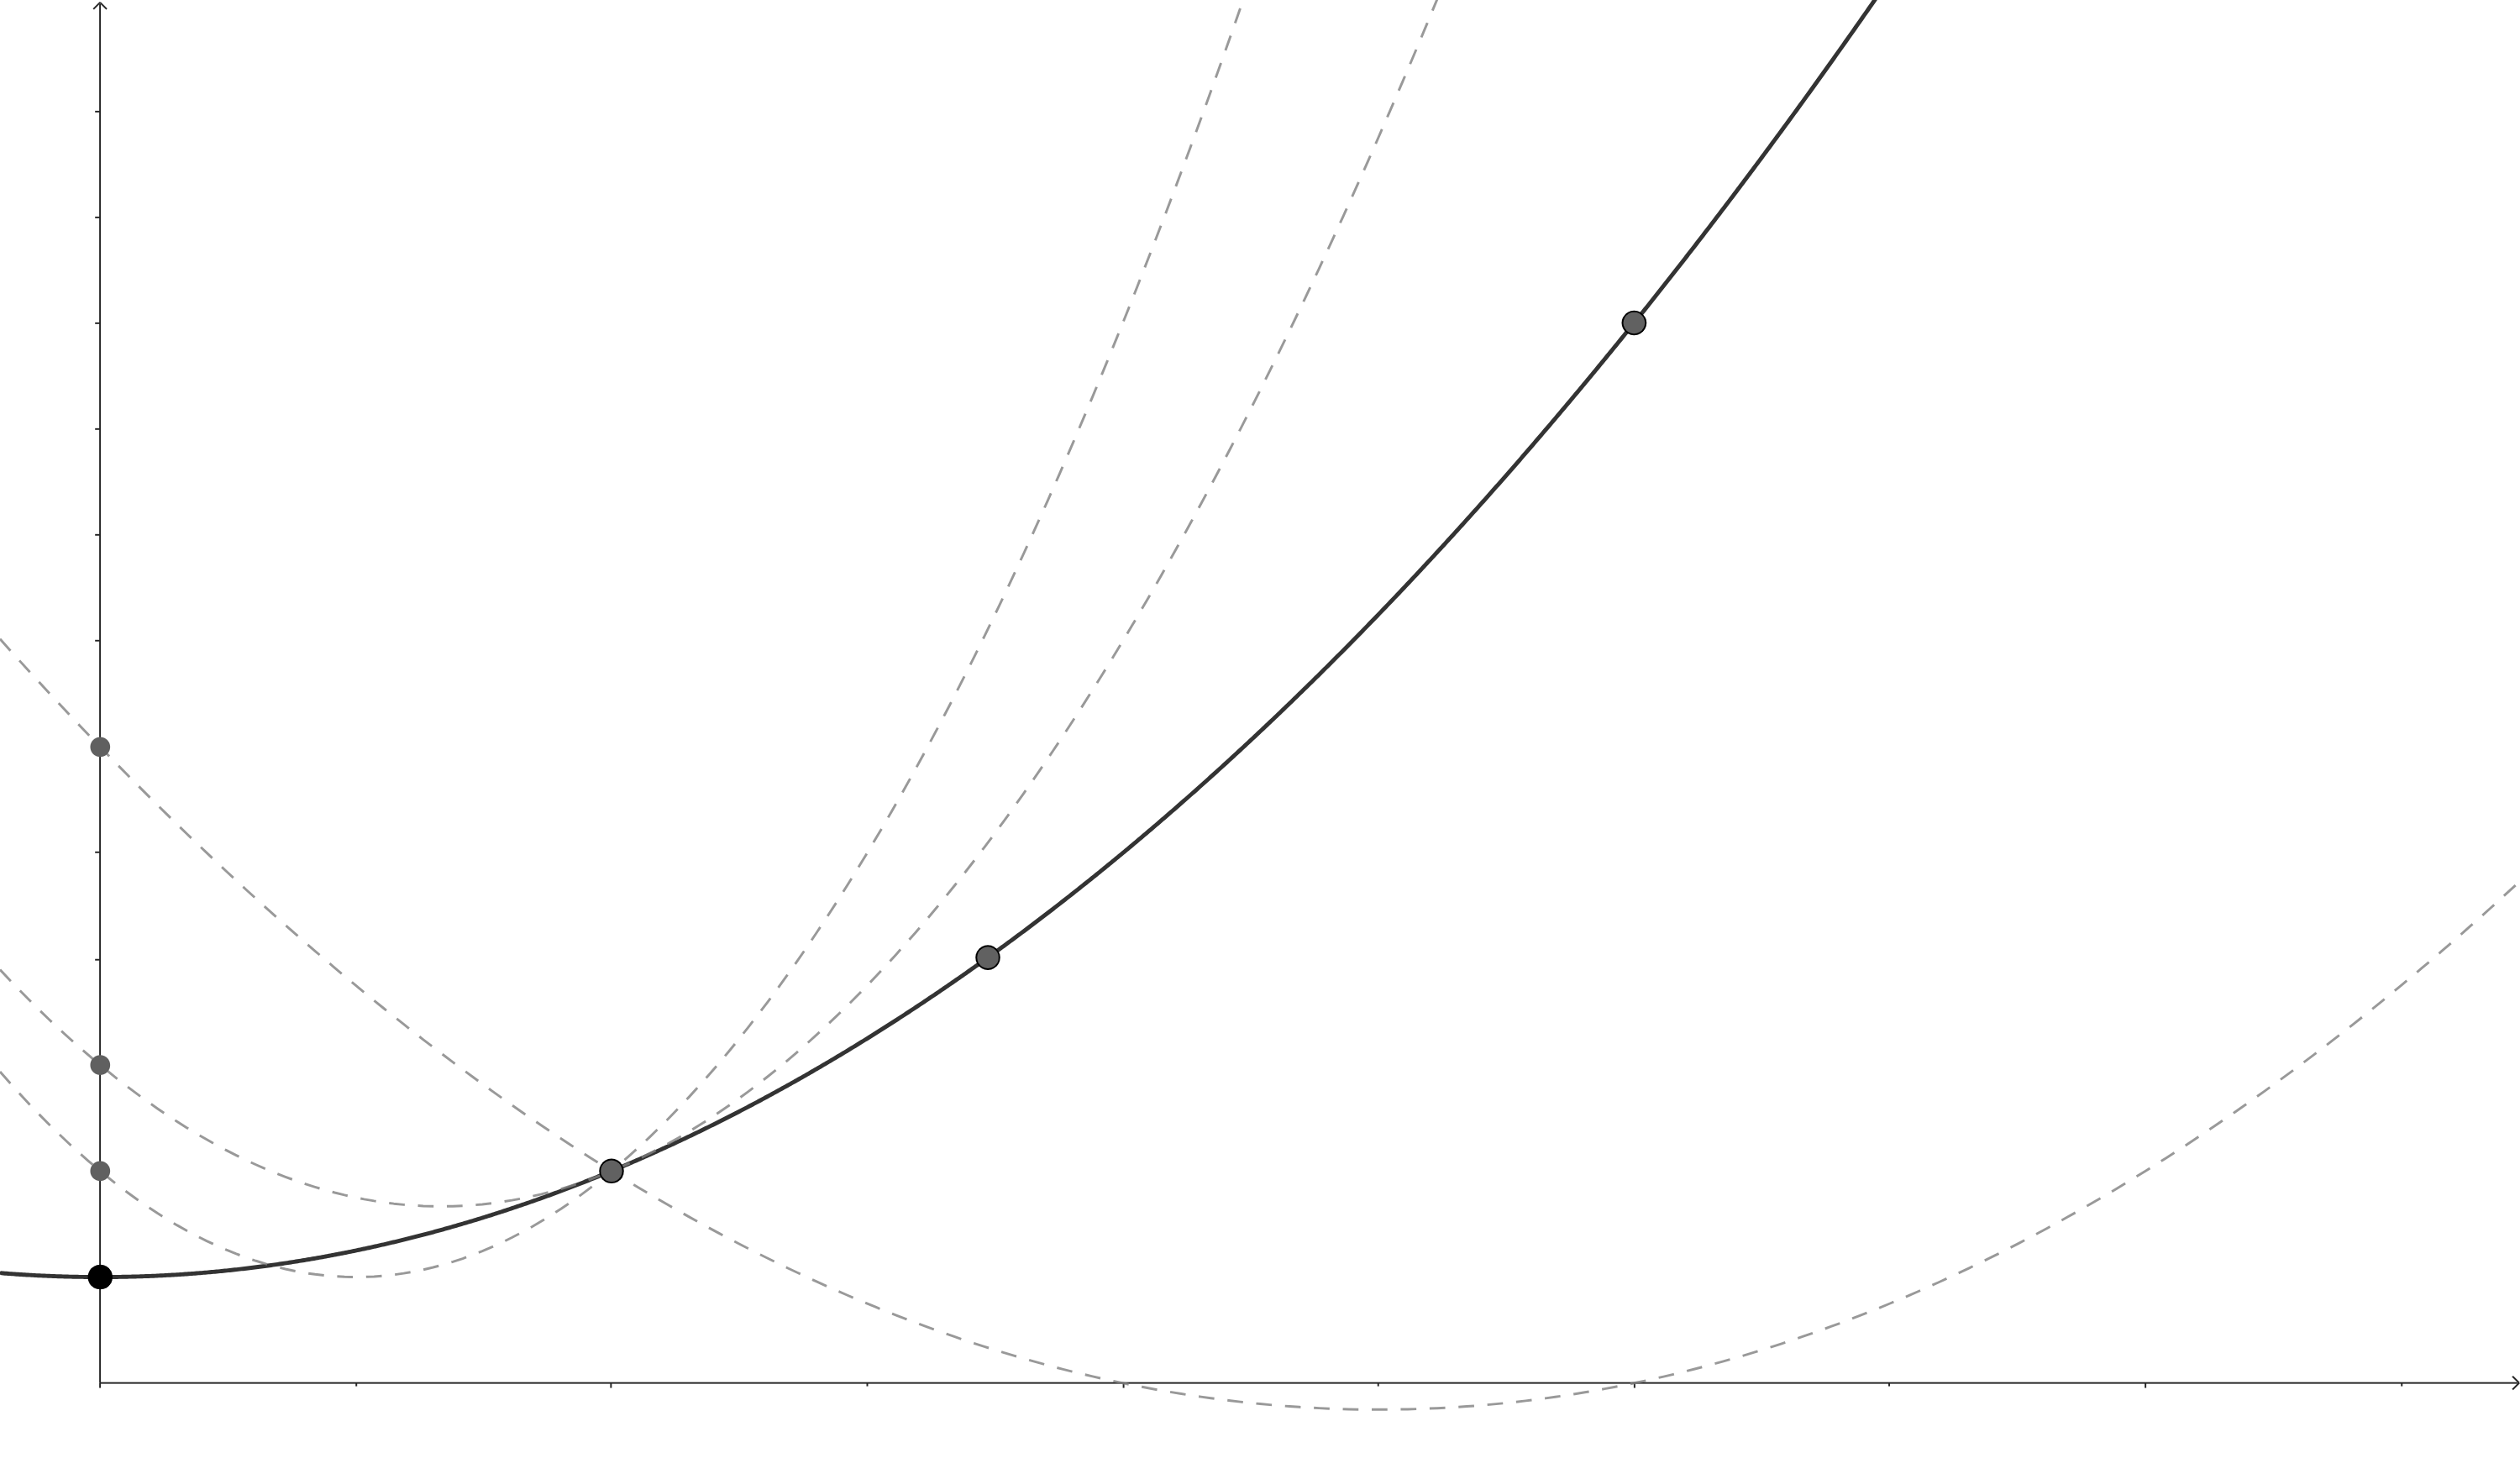
\includegraphics[width=0.8\textwidth]{images/shamir.png}
  \caption{Visualization of the Shamir's polynomial based secret sharing scheme. Each line shows a specific sharing instance for a secret $s$ and a threshold $\ell=2$. The sharing is kept secret for the threshold as two points can interpolate into several different secrets as shown by the dashed lines}\label{fig:shamir}
\end{figure}

\subsection{Secure Multi-Party Computation}\label{sec:mpc}

Secure Multi-Party Computation (MPC) refers to a cryptographic protocol enabling multiple parties to jointly compute a function $f$ represented by a circuit $C$, ensuring that no information about the individual inputs is revealed beyond what can be inferred from the output of $C$. In the following sections we will denote an MPC protocol by $f$ for an $N$-party functionality $f(x, w_1, \dots, w_n)$, a public input $x$ and secret inputs $w_i$ of the party $P_i$. The goal is to compute the function $f$ on the inputs of the $N$ parties while upholding the following properties~\cite{cramer2015secure}

\begin{definition}[Correctness]\label{def:mpc-correctness}
  We say that $\Pi$ realizes a deterministic $N$-party functionality $f(x, w_1, \dots, w_n)$ with perfect correctness if for all inputs $x, w_1, \dots, w_n$, the probability that the output of some player is different from the output of $f$ is negligible in the security parameter $k$, where the probability is over the independent choices of the random inputs $r_1, \dots, r_n$.
\end{definition}

\begin{definition}[Privacy]\label{def:mpc-privacy}
  The protocol ensures that no party learns anything about the inputs of the other parties beyond what can be inferred from the output of the function.
\end{definition}

\begin{definition}[$\ell$-privacy]\label{def:mpc-ell-privacy}
  The MPC protocol has privacy up to $\ell$ malicious parties.\footnote{Most often achieved by using an $(\ell + 1, N)$-threshold secret sharing scheme \autoref{def:mpc-ss-threshold}}
\end{definition}

In terms of security needed for the SDitH protocol, we define the following security requirements for the MPC protocol $f$

\begin{itemize}
  \item \textbf{Semi-honest security}: The protocol is secure against semi-honest adversaries, where parties follow the protocol but may attempt to learn information from the messages they receive.
  \item \textbf{Low-threshold security}: The protocol is secure against a coalition of up to $\ell$ parties, where $\ell$ is the threshold. This is also known as an $\ell$-private MPC protocol.
\end{itemize}

In order to prove the validity of an MPC protocol that have been run in the head/locally, we define the following notion of \textit{consistency}~\cite{ishai2007zero}.

\begin{definition}[MPC view]\label{def:mpc-view}
  We denote the view $V_i$ of a party $P_i$ in the protocol as $(i, x, r_i, w_i, (m_1, \dots, m_j))$ where $r_i$ is the randomness used by $P_i$, $w_i$ is the secret share, and $(m_1, \dots, m_j)$ are the messages received by $P_i$ in the first $j$ rounds of the protocol.
\end{definition}

\noindent Note that the messages sent by the parties can be inferred from the $V_i$ by invoking $\Pi$.

\begin{definition}[Consistent views]\label{def:mpc-consistent-view}
  We say that a pair of views $V_i, V_j$ are consistent (with respect to the protocol $\Pi$ and some public input $x$) if the outgoing messages implicit in $V_i, x$ are identical to the incoming messages reported in $V_j$ and vice versa.
\end{definition}

\begin{lemma}[Local and global consistency]\label{lem:consistency}
  Let $\Pi$ be an $N$-party protocol with a public input $x$. The following statements hold:
  \begin{enumerate}
    \item If all pairs of views $V_i$ and $V_j$ (for $i, j \in \{1, \dots, N\}$) are consistent with respect to $\Pi$, then there exists a full execution of $\Pi$ such that $V_i$ corresponds to the view of party $P_i$, for each $i$.
    \item Conversely, if such a full execution of $\Pi$ exists, then the pairwise consistency condition holds for all $V_i$ and $V_j$.
  \end{enumerate}
\end{lemma}

\textbf{Proof of \autoref{lem:consistency}} the first statement is trivial and follows from \autoref{def:mpc-view} and \autoref{def:mpc-consistent-view}.

The second statement is shown by the following. Consider $n$ pairwise consistent views $V_1, \dots, V_n$ \autoref{def:mpc-view}. Let us define an MPC protocol $\Pi$ by its \textit{next sent message} function $\Pi_j(i,x,w_i,r_i, (m_1, \dots, m_j)) = m_{j+1}$. The pairwise consistency, \autoref{def:mpc-consistent-view} and $\Pi_j$ implies, by induction that after $d$ rounds, that the actual view of all parties $P_i$ is the same as the view of $P_i$ in the first $d$ rounds. It follows that the views $V_i, \dots, V_n$ are consistent with the full execution of $\Pi$. \qed

This property is crucial as it enables a verifier in the MPCitH framework to validate the protocol's correctness.

\section{Syndrome Decoding Problem}\label{sec:syndrome}

The SDitH protocol is built on the computational hardness of the Syndrome Decoding (SD) problem for random linear codes over a finite field (see \autoref{sec:gf256}). Specifically, SDitH utilises a variant of the SD problem, referred to as the \textit{coset weights} problem, first introduced by Berlekamp and McEliece in 1978~\cite{berlekamp1978inherent}. We state the problem as follows:

\begin{definition}\label{def:syndrome}
  Given $H \in \mathbb{F}^{w\times m}_q$ and $y \in \mathbb{F}^{w}_q$. The problem is to find $x \in \mathbb{F}^m_q$ s.t.\ wt$(x) \leq w$, where $wt(x)$ denotes the Hamming weight, and $Hx = y$.
\end{definition}

Generating such an instance is straightforward: one can construct a uniformly random parity-check matrix $H$ and a codeword $x$ (with $wt(x) \leq w$), and then compute the syndrome $y = Hx$. In the SDitH protocol, the values of the matrix $H$ and the syndrome $y$ are elements of the finite field $\mathbb{F}_q$ explained previously in \autoref{sec:gf256}. The SD problem is well-known to be NP-complete for random instances~\cite{berlekamp1978inherent} also referred to as the \textit{general decoding problem}. To illustrate the computational difficulty, solving the problem using brute force would require $O(\binom{m}{w} q^w)$ operations, which is computationally infeasible for large enough $m$ and $w$.

\subsubsection{Standard form of the parity-check matrix}\label{sub:standard_form_of_the_parity_check_matrix}
To improve the performance and reduce the key size of the protocol, its possible to utilize the fact that the matrix $H$ can be in standard form. $H = (H'|I_{m-k}) $ Where $H' \in \mathbb{F}^{(m-k)\times k}_q$, and $I_{m-k}$ is the identity matrix of size $m-k$. This allows for the following representation of the syndrome:
\begin{equation}
  y = Hx = H'x_A + x_B\label{eq:standard_form_of_the_parity_check_matrix}
\end{equation}
with $x = (x_A | x_B)$. This improves the performance of the algorithms used in the SDitH protocol in the following ways
\begin{itemize}
  \item At the MPC layer, we only need to reveal one share $x_A$. Due to the fact that the other share $x_B$ can simply be recomputed by $x_B = y - H'x_A$.
  \item By linearity of the above relation one only needs to send $x_A$ in order to recover $Hx = H'x_A + x_B$, the Syndrome decoding instance. So from a sharing of $x_A$ one can check the correctness of the SD instance.
\end{itemize}

\subsubsection{Polynomial representation of SD}\label{sec:polynomial_representation}

The SDitH MPC protocol must prove that the SD problem $ y = Hx $ is satisfied. As outlined in \autoref{def:sdith-mpc}, the shared input $\sh{x_A}$ is provided to the MPC protocol. Consequently, the correctness of the initial statement $ y = Hx $ follows directly~\cite{feneuil2022syndrome}.

In addition to this, we need to verify that the Hamming weight condition $ \text{wt}(x) \leq w $ holds. To achieve this, the prover constructs three polynomials $ S $, $ Q $, and $ P $, alongside one public polynomial $ F $. The polynomials are defined as follows:

\begin{definition}[SDitH polynomials representation]\label{def:sdith-polynomials}
  Let $f_1,\dots, f_q$ denote all the elements of $\mathbb{F}_q$ and $x\in \mathbb{F}^m_q$ is a binary vector with Hamming weight $wt(x) \leq w$, then the polynomials are defined as:
  \begin{itemize}
    \item $S\in \mathbb{F}_q[X]$ is the Lagrange interpolation of the coordinates of $x$, such that it matches $S(f_i) = x_i$ for $i\in [1:m]$ and has degree $\text{deg}(S) \leq m-1$
    \item $Q\in \mathbb{F}_q[X]$ is defined by $Q(X) = \prod_{i\in E}(X - f_i)$. $E \subset [1:m]$ with order $|E| = w$, such that $E$ contains the non-zero coordinates of $x$. $Q$ has degree $\text{deg}(Q) = w$.
    \item $P\in \mathbb{F}_q[X]$ is defined as $P = S\cdot Q/F$ and has degree $\text{deg}(P) \leq w-1$. By definition the polynomial $F$ divides $S\cdot Q$.
    \item $F\in \mathbb{F}_q[X]$ is the \textit{vanishing polynomial} of the set ${f_1, \dots, f_m}$ also defined as $F(X) = \prod_{i\in [1:m]}(X - f_i)$ and has degree $\text{deg}(F) = m$.
  \end{itemize}
\end{definition}

\noindent We can now look at the relation
\begin{equation}
  \centering
  S\cdot Q = P\cdot F\label{eq:polynomial_representation}
\end{equation}

If we look at the left-hand side, which has the following property by design $S\cdot Q(f_i) = 0 \ \forall\ f_i \in [1:m]$. This comes from the fact that the polynomial $S(f_i) = 0$ whenever $x_i = 0$, as it is the Lagrange interpolation of $x$. Furthermore, the polynomial $Q(f_i)$ is zero whenever $f_i$ is a non-zero coordinate of $x$, which follows from the definition of $Q$.

For the right-hand side, the polynomial $F$ is the vanishing polynomial for the set ${f_1, \dots, f_m}$, so $F(f_i) = 0\ \forall\ f_i \in [1:m]$. The polynomial $P$ is needed to match the degree of $S \cdot Q$. As the degree of $F$ is $m \leq \text{deg}(S\cdot Q) \leq m + w - 1$.

It is now evident that if the prover can convince the verifier of the existence of polynomials $P, Q$ such that the relation $S \cdot Q = F \cdot P = 0$ holds at all points $f_i \in [1 : m]$, the following must be true: either $S(f_i) = x_i = 0$ or $Q(f_i) = 0$ for each $f_i$.

By the degree constraint of $Q$, the polynomial $Q$ can have at most $w$ roots (i.e., points $f_i$ where $Q(f_i) = 0$). Consequently, there are at most $w$ points where $S(f_i) \neq 0$, as $S(f_i)$ must be zero for all other $f_i$ to satisfy the given relation. This directly implies that $S$, and hence the vector $x$ it interpolates, has at most $w$ non-zero entries.

Thus, the weight constraint $\text{wt}(x) \leq w$ is satisfied, completing the proof. With this, we can define the soundness of the language for ZKP as follows:
\begin{equation}
  wt(x) \leq w \Leftrightarrow \exists P,Q \text{  with  }\text{deg}(P)\leq w-1\text{  and  }\text{deg}(Q) = w\text{ s.t. \autoref{eq:polynomial_representation} holds}\label{eq:soundness}
\end{equation}

\subsubsection{False positive probability}\label{sub:equality_test}
The equality test from \autoref{eq:polynomial_representation} has a small probability of false positives, denoted $p$. To reduce this probability, we can evaluate the relation at random points $\{r_k \in \mathbb{F}_q\}_{k\in[t]}$. By the Schwartz-Zippel \autoref{lem:schwartz}, the probability of a false positive is bounded by $p \leq \frac{t}{q}$, where $q$ is the size of the finite field $\mathbb{F}_q$. In short, this makes it unlikely that the relation will hold for all points $r_k$ if the relation is not sound according to \autoref{eq:soundness}. Furthermore, we can tweak the parameters $t$ and $q$ to reduce $p$.

\begin{lemma}[Schwartz-Zippel]\label{lem:schwartz}
  For a non-zero polynomial $P \in \mathbb{S}[X]$ of degree $d \geq 0$. Let $\mathbb{R}$ be a finite subset of $\mathbb{S}$ and set of random points $[r_1, \dots, r_n] \in \mathbb{R}$, the probability that $\Pr[P(r_1, \dots, r_n) = 0] \leq d/|\mathbb{R}|$.
\end{lemma}

\subsubsection{Avoiding interpolations for $S$}\label{sec:syndrome-avoid-interpolation}
Recall the sharing of the witness $\sh{x_A}$ for $x = (x_A \mid x_B)$ as described in \autoref{sec:syndrome}. In the current setup, each party in the MPC protocol would need to perform interpolation to compute their share $\sh{S}$. However, interpolation incurs quadratic complexity, leading to significant computational overhead. To address this issue, we redefine the SD instance as follows:

\begin{definition}[Redefined SD instance $y = Hx$]
  Let $s$ represent the coefficients of the polynomial $S$ in \autoref{eq:polynomial_representation}, and let $V$ be a matrix such that \[ S = \text{Lagrange Interpolation}(x) \Leftrightarrow s = Vx. \]
  The SD instance is then redefined as $y = HVx$.
\end{definition}

This redefinition preserves the security properties of the original SD problem, as the linear code $\mathcal{C}_{HV}$ remains uniformly random. This is due to the randomness of $\mathcal{C}_H$ and the invertibility of $V$.

With this modification, we can replace the sharing $\sh{x_A}$ with $\sh{s_A}$ by representing $s = (s_A \mid s_B) = Vx$. The parties can then compute $\sh{s_B}$ and $\sh{s}$ from the sharing of $\sh{s_A}$ using:
\[
  \sh{s_B} = y - H'\sh{s_A}.
\]
This modification significantly improves the efficiency of the MPC protocol and the computational overhead of the SDitH protocol.

\section{MPC-in-the-Head}\label{sec:mpcinth}

The SDitH protocol construction is built upon the \textit{Multi-Party Computation in the Head} (MPCitH) framework introduced by~\cite{ishai2007zero}. In this section, we provide an introduction to the MPCitH framework and demonstrate how it can be used to construct Zero-Knowledge Proofs of Knowledge (ZK-PoK). These proofs can then be combined with the \hyperref[sec:fiatshamir]{Fiat-Shamir heuristic} to derive a signature scheme. To begin, we first describe the concept of a ZK-PoK.

\subsubsection{Zero-Knowledge Proofs of Knowledge}\label{sec:zk}
The intuition behind a ZK-PoK is that a prover can convince a verifier that they know some secret $w$, such that $x$ is true, without revealing the secret $w$ to the verifier. For example, this could be someone wanting to prove that they are above the age of 18 without revealing their specific age.

\begin{definition}
  We denote a ZK-PoK $\Pi_{\mathcal{R}}$ for some \textbf{NP} relation $\mathcal{R} = \{(x, w)\; x \in L, w \in W(x)\}$.

  Let $x$ be a statement of language $L$ in \textbf{NP}, and $W(x)$ the set of witnesses for $x$ such that the following relation holds~\cite{feneuil2023threshold}   \[
    \mathcal{R}(x,w) = \begin{cases}
      1 & \text{if } x \in L \text{ and } w \in W(x) \\
      0 & \text{otherwise}
    \end{cases}
  \]  We have the following properties:
  \begin{itemize}
    \item \textit{Completeness}: If $x$ is true, then $\mathcal{R}(x, w)$ holds for some $w$.
    \item \textit{Soundness}: If $x$ is false, then the prover can convince the verifier that $\mathcal{R}(x, w)$ holds with negligible probability.
    \item \textit{Zero-knowledge}: The verifier learns nothing about the statement $x$.
  \end{itemize}
\end{definition}

\subsubsection{Generic ZK-PoK Construction}\label{sec:zk-generic}

The framework provides a versatile method for constructing ZK-PoK protocols. These protocols are typically considered quantum-safe because they can be built exclusively on symmetric-key assumptions, such as the hardness of inverting a cryptographic hash function, rather than on number-theoretic assumptions, such as factoring or discrete logarithms.

We will describe the basic construction suggested by Ishai et al~\cite{ishai2007zero}. For now, we will only consider an underlying semi-honest MPC protocol $\Pi_+$ for $N$ parties with $N-1$ secrecy based on \textit{additive} secret sharing -- see \autoref{sec:additive-sss}.

\begin{protocol}\label{def:mpcinth_basic}
  Given $\Pi_+$ a ZK relation $\mathcal{R}$ for some public statement $x$, and a witness $w$. Let $w_i$ be an additive secret share of $\sh{w}$ for the party $P_i$. Let \[ \Pi_+(x, w_1, \dots, w_n) = \mathcal{R}(x, w), \] i.e. $\Pi_+(x,w)$ outputs \texttt{Accept} if $\mathcal{R}(x,w) = 1$. We assume an underlying commitment scheme \texttt{Commit}.

  \begin{enumerate}[parsep=2pt, itemsep=0pt]
    \item The prover builds a random sharing of $\sh{w} = w_1, \dots, w_n$. Then
          \begin{enumerate}[nolistsep]
            \item Simulates the outputs of the MPC protocol $\Pi_+$ on the inputs $(x, w_1, \dots, w_n)$ and the randomness $r_1, \dots, r_n$.
            \item Prepares views $V_1, \dots, V_n$ of the parties in the protocol $f$.
            \item Commits to each view $V_i$ and sends ($\texttt{Commit}(V_1), \dots, \texttt{Commit}(V_n)$) to the verifier.
          \end{enumerate}
    \item The verifier picks $\ell$ random distinct indices $i \in [n]$ and sends them to the prover.
    \item The prover opens the corresponding $\ell$ commitments into the views $V_i$ and sends the openings to the verifier.
    \item The verifier accepts if and only if:
          \begin{enumerate}[nolistsep]
            \item\label{prop:mpcinth_commit} The views are consistent according to the commitment scheme.
            \item\label{prop:mpcinth_consistent} The views are consistent according to the public input $x$ and the randomness $r_1, \dots, r_n$.
            \item\label{prop:mpcinth_knowledge} The output of $\Pi_+$ from the views output \texttt{Accept}.
          \end{enumerate}
  \end{enumerate}
\end{protocol}

\noindent We see the following properties of the protocol:

\begin{lemma}[Completeness~\cite{ishai2007zero}]\label{def:mpcinth_completeness}
  Given an honest prover, $\mathcal{R}(x,w) = 1$ and the correctness of the MPC protocol $\Pi_+$, all outputs of $P_i$ are one and all views are consistent.
\end{lemma}

\begin{lemma}[Zero-Knowledge~\cite{ishai2007zero}]
  The verifier only sees $\ell$ views, and therefore from the definition of the MPC protocol $\Pi_+$ learns nothing of the secret witness $w$.
\end{lemma}

We consider soundness of the MPCitH framework. We assume that the verifier accepts the relation $\mathcal{R}(x,w)$ for $x \notin L$ -- i.e. the verifier accepts the relation even though the prover has created a false statement. This means that the prover must have cheated in one of two ways. First, the prover may have cheated in the underlying MPC protocol which is defined by the error probability $p$.

Secondly, the prover could have tampered with the views. In this, the prover must have corrupted one party and created a inconsistent view. The probability that the prover succeeds with this is at most $1 / N$. Giving an overall soundness of:

\begin{lemma}[Soundness of MPCitH for $\Pi_+$~\cite{feneuil2022syndrome}]\label{lem:soundness_mpcinth} Given a false positive probability $p$ for the underlying MPC protocol $\Pi_+$, the probability that the verifier outputs \texttt{Accept} for $\mathcal{R}(x,w) \neq 1$ is at most \[ \frac{1}{N} + p - \frac{1}{N} p \]
\end{lemma}


\section{Efficient product verification}\label{sec:mpc_sacrificing}

The basic MPCitH protocol serves as a foundation for constructing ZK-PoK for any \textbf{NP} relation and it has been demonstrated to yield relatively efficient ZK protocols~\cite{feneuil2022syndrome,baum2020concretely,katz2018improved}. Giacomelli et al. and Chase et al.~\cite{katz2018improved,giacomelli2016zkboo,chase2017post} provided concrete implementations of the \textit{MPC-in-the-Head} approach and observed that employing a 3-party MPC protocol achieved optimal performance within the space of protocols they analyzed.

However, due to the small number of parties, the soundness of the resulting protocols is relatively weak. Consequently, a large number of parallel repetitions is required to achieve a negligible soundness error. This significantly increases both the size of the proofs and the communication overhead of the protocols. In this section, we describe a variant of the MPC-in-the-Head protocol that is specifically sound for the addition relation.

In an effort to improve this, Baum and Nof introduced a variant of the framework based on a specialized MPC protocol. This protocol efficiently verifies a product relation $a \cdot b = c$. Their contributions significantly enhanced the efficiency of MPCitH-based ZK-PoK protocols and serve as the foundation for the underlying MPC protocol used in the SDitH protocol.

The underlying MPC protocol is based on arithmetic circuits, where addition operations are straightforward to perform using any $(+,+)$-homomorphic secret sharing scheme.

However, performing multiplication -- which is required for the product relation -- is significantly more challenging. The simplest approach would be to verify the relation by directly computing the product. A common technique for handling multiplication in MPC protocols is the use of Beaver triples.

\begin{definition}[Beaver triple~\cite{Beaver1992efficient}]\label{def:Beaver}
  A Beaver triple is a tuple $ (a, b, c) $ such that $ a \cdot b = c $, where $ a, b, c \in \mathbb{F}_q $.
\end{definition}

\begin{protocol}[MPC Multiplication using Beaver triples]\label{def:Beaver-multiplication}
  Given a $+$-homomorphic additive secret sharing scheme and a preprocessed random Beaver triple $\sh{a}, \sh{b}, \sh{c} $, the parties do the following:
  \begin{enumerate}[parsep=0pt, itemsep=0pt, topsep=0pt]
    \item The parties compute $ \sh{\alpha} = \sh{x} - \sh{a} $ and $ \sh{\beta} = \sh{y} - \sh{b} $.
    \item The parties run $ \text{open}(\sh{\alpha}) $ and $ \text{open}(\sh{\beta}) $ to obtain $ \alpha $ and $ \beta $.
    \item Each party computes $ \sh{z} = \sh{c} - \alpha \cdot \sh{b} - \beta \cdot \sh{a} + \alpha \cdot \beta $.
  \end{enumerate}
\end{protocol}


The above is a well-known technique from~\cite{Beaver1992efficient} where the correctness follows from the fact that
\begin{align*}
  \sh{z} & = \sh{c} - \alpha \cdot \sh{b} - \beta \cdot \sh{a} + \alpha \cdot \beta        \\
         & = \sh{ab} - (x - a) \cdot \sh{b} - (y - b) \cdot \sh{a} + (x - a) \cdot (y - b) \\
         & = \sh{xy}
\end{align*}

Proposals for ZK-PoK proofs -- such as the \textit{Cut-and-Choose} protocol~\cite{katz2018improved,baum2020concretely} -- utilize \autoref{def:Beaver-multiplication}, combined with preprocessing techniques, to achieve promising results (see appendix Appendix \ref{sec:zk-cut-and-choose}).

Building upon these protocols, Baum and Nof~\cite{baum2020concretely} propose a variant that shifts the focus from computing the product to simulating the \textit{verification} of the triple relation instead. This verification is performed by sacrificing another triple. Consider the following protocol, which is based on the MPC protocol described in~\cite{damgaard2012multiparty}.

\newpage
\begin{protocol}[Verification of a multiplication triple by sacrificing another]\label{def:sacrifice}
  Given an input triple $(x,y,z) \in \mathbb{F}$ random shared triple $(\sh{a}, \sh{b}, \sh{c}) \in \mathbb{F}$, it is possible to verify the correctness of the statement $z = x \cdot y$ without revealing any information on either of the input. Define \texttt{open} according to \autoref{def:ss-share}.
  \begin{enumerate}[parsep=0pt, itemsep=0pt, topsep=0pt]
    \item The parties generate a random $\varepsilon \in \mathbb{F}$.
    \item The parties locally set $\sh{\alpha} = \varepsilon\sh{x} + \sh{a}, \sh{\beta} = \sh{y} + \sh{b}$.
    \item The parties run \texttt{open}$(\sh{\alpha})$ and \texttt{open}$(\sh{\beta})$ to obtain $\alpha$ and $\beta$.
    \item The parties locally set $\sh{v} = \varepsilon\sh{z} - \sh{c} + \alpha  \cdot \sh{b} + \beta  \cdot \sh{a} - \alpha  \cdot \beta$.
    \item The parties run \texttt{open}$(\sh{v})$ to obtain $v$ and accept iff $v = 0$.
  \end{enumerate}
\end{protocol}

Observe that if both triples are correct multiplication triples (i.e., $z = xy$ and $c = ab$) then the parties will always accept since
\begin{align*}
  v & = \varepsilon \cdot z - c + \alpha \cdot b + \beta \cdot a - \alpha \cdot \beta                                                     \\
    & = \varepsilon \cdot xy - ab + (\varepsilon \cdot x + a)b + (y + b)a - (\varepsilon \cdot x + a)(y + b)                              \\
    & = \varepsilon \cdot xy - ab + \varepsilon \cdot xb + ab + ya + ba - \varepsilon \cdot xy - \varepsilon \cdot xb - ay - ab           \\
    & = (\varepsilon \cdot xy - \varepsilon \cdot xy) + (ab - ab) + (\varepsilon \cdot xb - \varepsilon \cdot xb) + (ya - ay) + (ba - ab) \\
    & = 0
\end{align*}

\begin{lemma}\label{lem:sacrifice_soundness}
  If $(\sh{a}, \sh{b}, \sh{c})$ or $(\sh{x}, \sh{y}, \sh{z})$ is an incorrect multiplication triple then the parties output \texttt{Accept} in the sub-protocol above with probability $\frac{1}{|\mathbb{F}|}$.
\end{lemma}

\textit{Proof}. Let $\Delta_z = z - x \cdot y$ and $\Delta_c = c - a \cdot b$. If the party accepts, then $v = 0$.
\begin{align}
  v & = \varepsilon \cdot z - c + \alpha \cdot b + \beta \cdot a - \alpha \cdot \beta                           \nonumber             \\
    & = \cdot (xy + \Delta_z ) - (ab + \Delta_c) + (\varepsilon \cdot x + a)b + (y + b)a - (\varepsilon \cdot x + a)(y + b) \nonumber \\
    & = \varepsilon\Delta_z - \Delta_c = 0 \label{eq:sacrifice-proof}
\end{align}

Consider the case where one of $\Delta_z$ or $\Delta_c$ is zero and the other is non-zero. In this case the verifier will not accept from~\ref{eq:sacrifice-proof}. Otherwise, we require that $\varepsilon = \Delta_c \cdot \Delta_z^{-1}$ which happens with probability $\frac{1}{|\mathbb{F}|}$. \qed

Under the MPCitH paradigm, the verifier must issue two challenges. The first challenge is for the randomness used in the MPC protocol computation, denoted by $\varepsilon$, which we refer to as the \textit{MPC challenge}. This challenge ensures that the prover cannot cheat in the computation of the multiplication gates or manipulate the inputs. By doing so, the verifier does not have to recompute the MPC inputs to check the consistency of the committed inputs, thereby significantly reducing the computational overhead for the verifier.

The second challenge is a \textit{view opening challenge} $I \subseteq [N]$, where $|I| = N-1$. This challenge is the same as the one used in the initial MPCitH protocol.

\section{Threshold Computation in the Head (TCitH)}\label{sec:threshold-mpc}

\autoref{def:sacrifice} forms the foundational mechanism underpinning the SDitH protocol. While this approach delivers significant improvements~\cite{baum2020concretely,feneuil2022syndrome} in efficiency and soundness for ZK-PoK protocols, further advancements can be achieved by revisiting the secret sharing schemes utilized within the MPCitH framework. The majority of constructions within the MPCitH framework~\cite{baum2020concretely,feneuil2022syndrome,katz2018improved} rely on $(N-1, N)$ additive SSS.

Recently, Feneuil and Rivain~\cite{feneuil2023threshold,feneuil2023threshold2} proposed the application of threshold SSS -- see \autoref{sub:threshold-sss}. For low-threshold SSS, their approach dramatically reduces computational overhead, as the prover emulates only $\ell + 1$ parties, while the verifier needs to verify and emulate just $\ell$ parties.

\begin{table}[]
  \centering
  \def\arraystretch{1.5}%  1 is the default, change whatever you need
  \begin{tabular}{ccc}
    \textbf{} & MPCitH                          & TCitH                                              \\ \arrayrulecolor{darkgray}\hline
    Prover    & $ \lambda \frac{N}{\log_2 N}$   & $ \lambda \frac{\ell + 1}{\log_2 \binom{N}{\ell}}$ \\ \arrayrulecolor{lightgray}\hline
    Verifier  & $ \lambda \frac{N-1}{\log_2 N}$ & $ \lambda \frac{\ell + 1}{\log_2 \binom{N}{\ell}}$ \\ \arrayrulecolor{darkgray}\hline
  \end{tabular}
  \caption{Performance for prover and verifier for TCitH compared to MPCitH. I.e. the approximate number of party emulations to achieve a soundness error of $2-\lambda$ (assuming a negligible false positive rate for the underlying MPC protocol)~\cite{feneuil2023threshold}.}\label{tbl:tcith-performance}
\end{table}

We define a threshold MPC protocol based on a $(\ell + 1, N)$-threshold SSS. In the context of the SDitH protocol, this can be instantiated with Shamir's Secret Sharing (\autoref{sub:shamir}).

On the other hand, the TCitH model~\cite{feneuil2023threshold} results in increased flexibility in the number of input shares the prover must open. While the prover still commits to all input sharings, only a subset of these needs to be opened during the protocol.

To facilitate this, a Merkle Tree Commitment Scheme (\autoref{sub:merkle_tree_prelim}) is employed. This scheme enables the prover to efficiently prove the consistency of a subset of committed inputs -- introducing a slight increase in communicational complexity.

\begin{lemma}[Soundness of TCitH based ZK-PoK]
  Given a $(\ell +1,N)$-threshold MPC protocol with false positive probability of $p_{\ell}$, we have a soundness error of
  \begin{align*}
    \frac{1}{\binom{N}{\ell}} + p_{\ell} \cdot \frac{\ell \cdot (N - \ell)}{\ell + 1}
  \end{align*}
\end{lemma}

\textit{Proof:} Soundness follows the same principle as before, with a slight modification. First, we assume that the MPC protocol has a perfect error rate $p_{\ell} = 0$.

We note that a malicious prover must tamper with exactly $N - \ell$ party emulations to successfully cheat the verifier. This can be shown by considering the case where the malicious prover attempts to cheat on fewer than $N - \ell$ parties. In such a scenario, at least $\ell + 1$ parties will have consistent views. Since $p_{\ell} = 0$, these consistent views define a valid witness $w$ such that $\mathcal{R}(x, w) = 1$, as required by the definition of the MPC protocol. Conversely, if the prover tampers with more than $N - \ell$ parties, the verifier will always detect the inconsistency.


Given $p_{\ell} = 0$ and the verifier opening $\ell$ inputs, the malicious prover can succeed in cheating the verifier with probability at most:
\begin{align*}
  \frac{1}{\binom{N}{\ell}}
\end{align*}

Now, consider the case where $p_{\ell} \neq 0$. The malicious prover may exploit the possibility of cheating the MPC protocol itself, resulting in a soundness error of:
\begin{align*}
  \frac{1}{\binom{N}{\ell}} + \left(1 - \frac{1}{\binom{N}{\ell}}\right) \cdot p_{\ell}.
\end{align*}

Finally, the malicious prover could provide an invalid sharing of the input witness $ \sh{w} $. Under such an attack, the final soundness error becomes:
\begin{align*}
  \frac{1}{\binom{N}{\ell}} + p_{\ell} \cdot \frac{\ell \cdot (N - \ell)}{\ell + 1} \geq \frac{1}{\binom{N}{\ell}} + \left(1 - \frac{1}{\binom{N}{\ell}}\right) \cdot p_{\ell}. \qed
\end{align*}

This final step is formally proven in~\cite[p20]{feneuil2023threshold} but we will go over the main ideas of the proof.

The first key observation is that the verifier only ever sees at most $\ell$ shares of the secret sharing $\sh{w}$. This limitation allows a malicious prover to construct multiple inconsistent sharings for subsets of $N$ parties while maintaining apparent consistency within any subset revealed to the verifier.

We define the set of all possible subsets of $N$ parties containing exactly $\ell + 1$ elements as:
\begin{align}
  \mathcal{J} = \{J \subseteq [N] \mid |J| = \ell + 1\}.
\end{align}

The malicious prover can then choose different witness values $w_J$ for each subset $J \in \mathcal{J}$, corresponding to shares $\sh{w}_J$. Specifically, the malicious prover selects:
\begin{align}
  w_{J_1} \neq w_{J_2} \quad \text{for } J_1, J_2 \in \mathcal{J}, \; J_1 \neq J_2.
\end{align}

\subsubsection{Soundness Attack Strategy}
This construction allows the malicious prover to perform a \textit{soundness attack}, where different witness values are sampled for each subset $J \in \mathcal{J}$. When the verifier sends a challenge value $\epsilon$, the malicious prover employs the following strategy:
\begin{itemize}
  \item \textbf{Case 1:} The challenge $\epsilon$ matches $w_{J_0}$ for some $J_0 \in \mathcal{J}$.
        In this case, the malicious prover defines the broadcast values and shares based on the subset $J_0$. This ensures that, for any subset $I \subseteq J_0$, the shares appear consistent to the verifier.

  \item \textbf{Case 2:} The challenge $\epsilon$ does not match any $w_{J_0}$.
        If no subset $J_0$ contains a witness value matching the challenge $\epsilon$, the malicious prover must guess which subset $I$ the verifier will check. If the guess is incorrect, the inconsistency will be detected.
\end{itemize}

The authors prove that the above strategy is optimal for the malicious prover and that the probability of success matches the previously analyzed bound. Showing that the success of such a strategy is directly tied to the security of the underlying commitment scheme, and any efficient prover capable of consistent cheating would break the commitment scheme.

As a result, the protocol's soundness holds under the assumption that the commitment scheme is secure.


\section{Fiat-Shamir Heuristic}\label{sec:fiatshamir}
To transform any ZK-PoK protocol into a signature scheme, one can use the approach described in~\cite{fiat1986prove}. Here, we outline the general concept.

ZK-PoK interactive protocols, such as the MPCitH protocols discussed above, depend on the verifier to issue a challenge to the prover. This challenge acts as a source of randomness, which the prover cannot control.

To adapt such a protocol into a signature scheme, the prover must eliminate the verifier's role in providing the randomness. This is achieved by allowing the prover to independently generate the challenge using a pseudo-random function, such as a collision-resistant hash function. By modeling the hash function as a random oracle, its security guarantees ensure that the prover cannot manipulate the randomness of the verification challenge. This maintains the fundamental property of ZK-PoK interactive protocols while enabling the transformation into a non-interactive signature scheme.

Within the context of the SDitH protocol, the transformation from a ZK-PoK to a signature scheme is accomplished by substituting the verifier's \textit{MPC challenge} and \textit{view opening challenge} with the output of a hash function, where the hash function take as input the prover's prior communications.

\section{The Rust Programming language}\label{sec:rust}
As a preliminary to our implementation, we need to answer the question: ``Why is Rust a good choice for PQC?''.

In 2024, the government of the United States of America took a stance on the future of cyber secure programming languages~\cite{whitehouse2024memorysafe}. In their report, they underline the need for secure building blocks when developing secure software. They point to the fact that \textit{Common Weakness Enumeration} (CWE) data highlights \textit{memory safety vulnerabilities} (MSV) as one of the most pervasive classes of vulnerabilities. MSV's exploit how memory can be accessed, written, allocated, or deallocated in ways that are beyond the scope of the program. Common examples of programming languages that are vulnerable include C and C++, which are widely used due to their high performance. To prevent such vulnerabilities, the report emphasizes the importance of using programming languages that inherently provide memory safety and does not require the developers to manually ensure security.

The Rust programming language addresses memory safety through its unique \textit{borrow checker}~\autoref{sec:rustborrow}, which enforces strict rules on how memory is accessed and managed. In the same year as the White House's report, NIST also released their recommendations on \textit{Safer Languages}~\cite{nistsaferlanguages}, which highlighted Rust as a potential choice. Together, these endorsements underscore that Rust is well-suited for implementing a protocol that must adhere to modern security standards.

In addition to its focus on safety, Rust benefits from an extensive library of community-maintained documentation and resources~\cite{rustlangRustProgramming,rustlangPerformanceBook,lurklurkEffectiveRust}. These resources provide invaluable support for developers, enabling them to better understand the language's features and effectively utilize its capabilities.

In this section, we provide an overview of the key features of the Rust programming language that will be utilizing in this project. Specifically, how we might leverage Rust's safety mechanisms, performance optimization capabilities, dynamic language features, and robust testing infrastructure.

\subsection{Cargo - Rust package manager}\label{sec:cargo}
A Rust program, referred to as a \textit{crate}, is typically compiled using the Rust Compiler with a command such as \texttt{rustc hello.rs}. However, manually managing versions and dependencies can be tedious and error-prone. To simplify this process, Rust provides a \textit{package manager} called Cargo~\cite{rustlangCargo}.

Cargo is a command-line tool -- run through \texttt{cargo} -- that facilitates the management of dependencies, building, testing, and benchmarking of your crate, as well as generating documentation. It is the officially recommended method for managing and building Rust projects.


\subsection{Memory safety}\label{sec:rustborrow} % mut references
Rust guarantees both type safety (\autoref{sub:rusttypes}) and memory safety. While we will not delve into the details, significant progress has been made toward formal proofs of these guarantees~\cite{jung2017rustbelt}. Unlike many other languages that rely on sophisticated garbage collection mechanisms to ensure memory safety, Rust avoids the associated performance overhead through two key features: \textit{ownership} and \textit{lifetimes}. Along with a compile time functionality called the \textit{borrow checker}.

While the borrow checker is often the biggest challenge for new Rust developers, it is also the feature that makes Rust exceptionally powerful for secure applications.

In this section, we will explore the fundamental aspects of how the borrow checker and ownership work. We will focus on the most critical aspects, as more comprehensive information is available in the official documentation~\cite{rustlangRustProgramming}.

\subsubsection{Data Race Vulnerability}
\textit{Data races} are similar to race conditions and occur when
\begin{enumerate}[parsep=0pt, itemsep=0pt, topsep=0pt]
  \item Two or more pointers access the same memory location concurrently,
  \item At least one of the pointers is used to write to the memory location, and
  \item There is no mechanism to synchronize the data access.
\end{enumerate}

Data races most often result in undefined behavior that can crash a program. However, they can also introduce severe security vulnerabilities, which malicious actors may exploit\footnote{e.g., \href{https://nvd.nist.gov/vuln/detail/cve-2024-35898}{CVE-2024-35898}}.

In Rust, the borrow checker ensures that data races cannot occur by diagnosing them at compile time and preventing the program from compiling if such conditions are detected.

\subsubsection{The Stack and Heap}
To understand how Rust manages memory, it is first essential to grasp the distinction between the stack and the heap. These are two memory management systems available at runtime~\cite[ch.4]{rustlangRustProgramming}, each with unique characteristics and use cases.

\begin{definition}[The Stack]
  The stack stores values in a last-in-first-out (LIFO) order, meaning the last value added is the first to be removed. All data stored on the stack must have a fixed, known size at compile time. This gives the stack its \textit{fixed-sized} structure.
\end{definition}

\begin{definition}[The Heap]
  The heap, in contrast, is more flexible. When you allocate memory for a value on the heap, you request a specific amount of memory, and the heap manager finds a suitable location for it. A helpful analogy for the heap is docking a spaceship on Coruscant: you tell the spaceport how large your ship is, and they assign you to a landing pad that fits your ship's dimensions, noting where you've been docked.
\end{definition}

\subsubsection{Performance versus Dynamism}

Between the two memory allocations there exists a \textit{performance versus dynamism} trade-off. Consider the following code example:

\begin{minted}{rust}
  let a: Vec<u8> = vec![1, 2, 3];
  let b: [u8; 3] = [1, 2, 3];
\end{minted}

This code demonstrates two data types being allocated. The first, \rust{a}, is a vector type, while the second, \rust{b}, is a fixed-size array type. The vector type is always allocated on the heap, whereas the fixed array is allocated on the stack. Pushing and accessing the stack is faster than using the heap. Therefore, keeping values on the stack tends to outperform heap allocations. This is because heap allocation involves searching for a suitable location in memory to store the data.

Furthermore, the heap is slower because you have to follow a pointer from the stack to the allocated data. Note that there are several optimisations you can do when allocating to the heap, like changing the allocator for specific use cases, instantiating the vector with a capacity or the \rust{SmallVec} that dynamically changes from the stack to the heap when allocation surpasses its defined capacity. See~\cite{rustlangPerformanceBook} for more.

However, the vector type is far more dynamic. For instance, using the \rust{push} method, you can add more elements to a vector, and the allocator will automatically find additional space on the heap if needed. Conversely, stack allocations in Rust require that the size of the data is known at compile time, which imposes significant restrictions on how dynamic your code can be. This limitation became particularly evident when designing around the different category variants in \autoref{sub:constants}. However, this also ensures at compile time that you cannot access memory outside of the stack, a common vulnerability exposed in C/C++.

Additionally, the stack, due to its fixed-size structure, can only hold a limited amount of data. Attempting to allocate more memory than the stack can accommodate results in a \textit{stack overflow} error. In contrast, the heap offers virtually unlimited storage, as it can dynamically allocate memory as required.

\subsubsection{Ownership and Variable scope}
Now that we have given a brief introduction to the memory allocation, we can delve into the \textit{ownership system}. This system is a crucial aspect of Rust's memory management, as it ensures that memory is allocated and deallocated correctly. Ownership in Rust follows three rules
\begin{enumerate}[parsep=0pt, itemsep=0pt, topsep=0pt]
  \item Each value has an \textit{owner}
  \item There can only be one owner at a time
  \item When an owner goes out of scope, the value will be \textit{dropped}.
\end{enumerate}
First, we consider the \textit{variable scope} in the following example
\begin{minted}{rust}
{
  // d is inaccessible before it has been assigned to the current scope
  let d = "Peace is a lie";
  println!("{d}") // Now we can use d
} // d is dropped here
\end{minted}
In this example, the variable \rust{d} comes into the scope and remains valid until the scope is closed. This is similar to most other programming languages. This works because the string literal \rust{"Peace is a lie"} is of known size at compile time and is allocated on the stack, meaning that it can be easily copied on stack and popped when the current scope ends. It also means that while it is efficient and fast, the variable \rust{d} cannot be mutated after the fact.

\subsubsection{Variable and data interaction with \textit{Move}}

To illustrate where Rust differs, we need a data type that is more complex and stored on the heap instead. We will change the example to use a \rust{String} type

\begin{minted}{rust}
  let mut d = String::from("Peace is a lie");
  d.pust_str(", there is only passion."); // We can mutate d
  println!("{d}"); // > "Peace is a lie, there is only passion."
\end{minted}

A variable instantiated with the \rust{String} type is dynamically allocated on the heap, and a \textit{pointer} is instead saved on the stack. Now consider both types of assignments with a \textit{re-assignment}

\begin{minted}{rust}
  // Case 1: Stack allocated type
  let d = "Through passion, I gain strength"
  let v = d;

  // Case 2: Heap allocated type
  let d = String::from("Through strength, I gain power");
  let v = d;
\end{minted}

For Case 1, if the string literal \rust{d} implements the \textit{Copy} trait. This means that when we assign \rust{let v = d}, its value can be copied onto the stack with a negligent performance hit. This means \rust{d} remains accessible after being used or assigned elsewhere because its data was duplicated. Due to the immutability and fixed size of the string literal, this operation is also memory safe.

However, for Case 2; The variable \rust{d} is instead a \textit{pointer} to a heap-allocated string, it resides on the stack but points to data stored on the heap. When \rust{d} is moved to another variable (e.g., \texttt{v}), the pointer itself is transferred to \texttt{v} and the heap-allocated data remains unchanged. Ownership of the pointer is moved to \texttt{v}. This is called a \textit{move}. After the move, \rust{d} is no longer valid, and any attempt to use it would result in a compile-time error.
\begin{minted}{rust}
  let d = String::from("Through strength, I gain power");
  //  ^ move occurs because `d` has type `String`, which does not implement the `Copy` trait
  let v = d;
  //      ^ value moved here
  println!("{d}"); 
  //        ^^^ value borrowed here after move
  // error[E0382]: borrow of moved value: `d`
\end{minted}

\subsubsection{Why the Restriction?}

Allowing \rust{d} to be used after the move could lead to undefined behavior, such as a \textit{double free} memory safety bug, as both \rust{d} and \rust{v} would attempt to drop the same data. Additionally, simultaneous access or modification of heap-allocated data could cause data races. To prevent such issues, Rust enforces these ownership rules at compile-time. If \rust{d} needs to be used after a move, the heap data must be explicitly \textit{cloned} before transferring ownership, ensuring safe and predictable memory usage.

\subsubsection{Function ownership}\label{sub:rustlifetimes}
Now that we have covered the basics of ownership, we explore how it interacts with functions. When passing a value to a function, the function takes ownership of the value. This means that the function takes over managing the \textit{lifetime} of the value, ensuring that it is not used after the function call, unless it is copied.

For stack allocated types, the structure of the stack and known compile time size, nothing special needs to happen when the function exits. However for heap allocated types
\begin{minted}{rust}
  fn takes_ownership(some_string: String) { // some_string comes into scope
    println!("{some_string}");
  } // Here, some_string goes out of scope and `drop` is called.
    // The memory on the heap is freed.
\end{minted}

The function takes ownership of the \rust{String} value \rust{some_string}. When the function ends, the \rust{String} value is dropped, and the memory on the heap is freed. This is because the value is no longer valid after the function call has ended.

However, a function can also take ownership of a value. Here's an example where the function takes ownership of the value and then transfers the ownership back to a new variable \rust{v} making the old allocation invalid.
\begin{minted}{rust}
  fn main() {
      let d = String::from("hello");
      let (v, len) = calculate_length(d);
//                                    - value moved here
       println!("The length of '{v}' is {len}."); // v is valid
       println!("The length of '{d}' is {len}."); // d is no longer valid
//                              ^^^ value borrowed here after move
  }

  fn calculate_length(s: String) -> (String, usize) {
    let length = s.len();
    (s, length)
  }
\end{minted}

\subsubsection{Borrowing with references}
However, often it is tedious to keep transferring ownership of values, whenever they need to be used in a function. Rust provides a way of avoiding this transfer of ownership by using \textit{references}. References allow you to \textit{borrow} the value without taking ownership of it. This is done by using the \rust{&} symbol. Consider the same augmented example
\begin{minted}{rust}
  fn main() {
    let d = String::from("hello");
    let len = calculate_length(&d);
    println!("The length of '{d}' is {len}."); // d is valid
  }
\end{minted}

In this way, the function variables \rust{s} never takes ownership of \rust{d}, meaning that it is not dropped when the function call ends. We call the action of creating a reference \textit{borrowing}.

\subsubsection{Mutable references}
However references have their limitations. The reference is immutable, meaning that we cannot modify \rust{s}. If we wanted to modify the value, we would need to use a \textit{mutable reference}.

\begin{minted}{rust}
  fn main() {
    let mut d = String::from("hello");
    modify(&mut d);
  }
  
  fn modify(s: &mut String) {
      s.push_str(", world");
  }
 \end{minted}

With the \rust{&mut} annotation we tell the compiler that we want to modify the value. This is a powerful feature, but it comes with restrictions. If you have a mutable reference to a value, you can have no other references to that value to prevent data races.
\begin{minted}{rust}
  let mut s = String::from("hello");

  let r1 = &s;
  //       ^^^^^^ immutable borrow occurs here
  let r2 = &mut s;
  //       ^^^^^^ mutable borrow occurs here

  println!("{}, {}", r1, r2);
  //                 ^^ immutable borrow later used here
  // error[E0502]: cannot borrow `s` as mutable because it is also borrowed as immutable
\end{minted}
The compiler eases these restrictions as it can determine the lifetime of the references. Consider the following example
\begin{minted}{rust}
  let mut s = String::from("hello");

  let r1 = &s; // no problem
  let r2 = &s; // no problem
  println!("{r1} and {r2}");
  // variables r1 and r2 will not be used after this point

  let r3 = &mut s; // no problem
  println!("{r3}");
\end{minted}
The last borrow is valid because the previous borrows are no longer in scope. The compiler can determine that the borrows will not be used after the last borrow.

\subsubsection{Lifetimes}
The \textit{lifetime} of a value on the stack refers to the period during which the value is guaranteed to remain valid within its scope. In most cases, developers do not need to actively manage lifetimes, as the compiler can infer them automatically. A value's lifetime begins when it is assigned ownership and ends either when it is dropped or when its ownership is transferred.
\begin{minted}{rust}
  let r: &Item;
  {
    let item = Item { contents: 42 };
    //  ^^^^ binding `item` is declared here
    r = &item;
    //  ^^^^^ borrowed value does not live long enough
  }
  println!("r.contents = {}", r.contents);
  //                          ^^^^^^^^^^ borrow later used here
  // error[E0597]: `item` does not live long enough
\end{minted}
While the Rust compiler, most often can infer the lifetime of a value it can sometimes be necessary to explicitly define the lifetime. This is done by using the \textit{lifetime annotation} \rust{'a}. Consider the example below
\begin{minted}{rust}
  pub fn find(haystack: &[u8], needle: &[u8]) -> Option<&[u8]> 
    //                  -----          -----            ^ expected named lifetime parameter
    // ... // error[E0106]: missing lifetime specifier
\end{minted}
There are two choices for the output lifetime for the reference returned by the function. The compiler cannot infer which lifetime to use, so it requires the developer to specify it. This is done by adding the lifetime annotation to the function signature.
\begin{minted}{rust}
  pub fn find<'a, 'b>(haystack: &'a[u8], needle: &'b[u8]) -> Option<&'a[u8]>
\end{minted}
In the example above, we define two generic lifetimes, \rust{<'a, 'b>}, ensuring that the lifetime of $h$ is $'a$. This allows the compiler to verify that $h$ lives long enough. Additionally, the compiler infers that the output reference shares the same lifetime as the input reference \rust{haystack}.

\subsubsection{Conclusions on Memory Safety in Rust}
This overview only touches on the features that make Rust a powerful programming language for developing secure and high-performance software. While Rust has a steep learning curve, its large and active community provides extensive documentation and resources. Readers are encouraged to explore the official Rust Book~\cite{rustlangRustProgramming} or community-authored books such as \textit{Effective Rust}~\cite{lurklurkEffectiveRust} and \textit{The Rust Performance Book}~\cite{rustlangPerformanceBook}.

\subsection{Correctness (Types, Testing and Error handling)}
When developing and iterating on software, it is essential to ensure the continuous delivery of functional and correct code. Various patterns can help achieve this, and Rust provides several. In this section, we will focus on three: Types, Automated Tests, and Error Handling.

\subsubsection{The Type System}\label{sub:rusttypes}
Every value in Rust has a \textit{data type}. Programs written in Rust are \textit{statically typed}, meaning the type of each value must be determined at compile time. The type informs the compiler about what operations the value supports and helps catch errors before they reach runtime~\cite[ch.3.2]{rustlangRustProgramming}. The Rust compiler often infers types automatically, but if it cannot, you must explicitly annotate the type of the value. Consider the following example:

\begin{minted}{rust} 
  let guess: u32 = "42".parse().expect("Not a number!"); 
\end{minted}

Here, the \rust{parse} function requires the annotation of the variable \rust{guess} to determine how the string should be parsed. Additionally, if you annotate \rust{guess} with a type that does not implement the \rust{parse} function for strings, the compiler will produce an error.

The type system ensures that Rust minimizes the possibility of writing incorrect code -- at least in terms of the bounds of the language and the program. While Rust enforces correctness in type usage, ensuring that a program operates semantically as intended, such as adhering to a protocol specification, often requires additional validation methods.

\subsubsection{Automated Testing}
Say that you are implementing field arithmetic -- \textit{funny enough, we needed to do exactly that!} -- you would want your implementation to follow the properties that define the field. For example \textit{associativity over addition}
\begin{align}
  a + (b + c) = (a + b) + c
\end{align}
Such a property is hard to enforce using the type system. However, it is possible to enforce it using \textit{automated testing}. Consider the following examples

\begin{minted}{rust}
  fn gf256_add(a: u8, b: u8) -> u8 {
    a ^ b
  }

  #[cfg(test)]
  mod arithmetic_tests {
    use super::*
    
    #[test]
    fn test_add_associativity() {
      let a = 3;
      let b = 4;
      let c = 5;

      assert_eq!(
        gf256_add(gf256_add(a, b), c), 
        gf256_add(a, gf256_add(b, c))
      );
    }
  }
\end{minted}

This example demonstrates how straightforward automated testing is in Rust. First, we create an internal module, \rust{mod arithmetic_tests}, with the annotation \mintinline{rust}|#[cfg(test)]|. This annotation ensures that the module is included only during testing and excluded from the final production code.

Individual tests are made using the \mintinline{rust}|#[test]| and a function. Then we can use the macro \rust{assert_eq!()} to test whether or not the property is upheld.

To run the tests in our implementation you simply run the following
\begin{minted}{bash}
  $ cargo test
  running 1 test
  test gf256::arithmetic_tests::test_add_associativity ... ok
\end{minted}
This test ensures we can continue developing or optimizing the finite field while verifying its validity. Rigorous testing simplifies debugging and helps catch potential issues early.

Writing good tests is a broad topic beyond the scope of this report. However, our implementation was designed with testing in mind, enabling iterative development while ensuring each module aligns with theoretical expectations and the given specification.

\subsubsection{Error handling}\label{sub:rusterror}
Testing that functions return correct values for \textit{valid} inputs is essential for ensuring correctness. But how should unexpected inputs, such as those provided by a user to a CLI, be handled? In Rust, errors can be managed in two ways:
\begin{itemize}[itemsep=0pt, topsep=0pt, parsep=0pt]
  \item \rust{panic}: Stops the program's execution.
  \item \rust{Result<T, Err>}: Wraps the return value with an error type, allowing the caller to handle the error.
\end{itemize}
So, when should you use \rust{panic}? You should panic only if your code reaches an unrecoverable state~\cite[ch.9.3]{rustlangRustProgramming}. Otherwise, it is better to use \rust{Result} to enable the caller to handle errors in a way that suits their use case.

\begin{minted}{rust}
  fn sign(message: &[u8], secret_key: &[u8]) -> Result<Vec<u8>, Error> {
    if secret_key.len() == 0 {
      return Err(Error::SigningError);
    }
    ... code that signs the message ...
    Ok(signature)
  }

  fn main() {
    let message = b"Hello, World!";
    let sk = b"...";
    let signature = sign(&message, &sk);

    // You can match on the result to handle the error
    match signature {
      Ok(signature) => println!("Signature: {:?}", signature),
      Err(e) => eprintln!("Error: {:?}", e),
    }

    // or you can use the methods supplied by the Result type
    if (signature.is_ok()) {
      println!("Signature: {:?}", signature.unwrap());
    } 
  }
\end{minted}
There are several reasons why a signature might fail to generate, but a straightforward one to communicate to the user is an invalid secret key. In this case, we return an error with the \textit{SigningError} variant. Using a \rust{panic} would prevent the caller from recovering from the error.

\subsection{Maintainable and readable code}

A key goal of this project was to create an implementation that is easy to read, enabling future implementers to understand the protocol. Rust was chosen in one part for its robust set of tools and features, which facilitate writing maintainable and readable code.

\subsubsection{Code Documentation}\label{sub:code-documentation}
First things first, good written code should either be written in a way so that it is self-explanatory or the developer should instead supply the necessary documentation in order for the reader to quickly grasp the concepts and functionality.

Often times you would want to supply documentation in the form of comments, above functions and variables to explain their purpose and functionality. Furthermore, you would want to supply the user with a \textit{manual} where the user can read about the exposed library.

It can be hard to maintain both of these aspects separately. Rust enables the developer to write both at the same time. Consider the following code in a module

\begin{minted}{rust}
  //! This module exposes two functions: add and double

  /// Adds two functions together
  pub fn add(a: u8, b: u8) -> u8 { 
    a + b
  }

  /// Doubles a number using [`add`]
  pub fn double(a: u8) -> u8 {
    add(a, a)
  }
\end{minted}

Adding a triple slash \rust{///} above a function or struct generates documentation for it. Hovering over the function in most Rust-compatible editors, such as \href{https://code.visualstudio.com/docs/languages/rust}{Visual Studio Code}, displays the documentation. Similarly, using \rust{//!} creates top-level documentation for the module.

While these comments enable developers to access documentation directly within the code, Rust also provides a powerful feature to automatically generate comprehensive documentation. By running \href{https://doc.rust-lang.org/cargo/commands/cargo-doc.html}{\texttt{cargo doc}}, you can create a webpage with detailed documentation for the project. Checkout out the documentation for our project \href{https://mactherobot.github.io/sdith-rust}{here}.

\subsubsection{Codebase structure and Modules}\label{sub:rust_modules}
Rust provides a module system that allow you to organize your code into logical units. Making it easier to understand and maintain the codebase. A module is a collection of related items, such as functions, structs, and constants, that are grouped together. They can be nested, allowing for a hierarchical structure of code.
If utilized correctly, this can help organize the logic of a program effectively for readability and reuse. For example, encapsulating field arithmetic within a module and separating components into subfolders and subroutines related to the main signature algorithm.

Rust structures modules either directly in the code or through the file system. There are two files that provides the entry points to your program
\begin{enumerate}
  \item \texttt{main.rs}: This is the main entry point of the program. It is the first file that is executed. You can quickly run the program by running \texttt{cargo run}.
  \item \texttt{lib.rs}: In the case that you are building code that you want to provide for other developers to use in their own Rust code -- named a \textit{crate} -- this is the entry point for such a library.
\end{enumerate}

Consider a simple example structure below

\begin{minted}{rust}
  // main.rs
  use crate::arith::gf256::add;

  mod arith

  fn main() {
    println!("{}", add(3, 4));
  }

  // arith.rs
  pub mod gf256;

  // arith/gf256.rs
  pub fn add(a: u8, b: u8) -> u8 {
    a ^ b
  }

  #[cfg(test)]
  mod tests {
    ...
  }
\end{minted}

The example shows a structure with the main entry file which first declares a module \rust{mod arith}. The compiler then looks for the code of the module in three places
\begin{itemize}[parsep=0pt, itemsep=0pt]
  \item Inline with curly braces (e.g. like the \rust{mod tests {}})
  \item In the file \texttt{arith.rs}
  \item In the file \texttt{arith/mod.rs}
\end{itemize}
In this case, the module \rust{arith} is declared in the file \texttt{arith.rs}. A nested submodule \rust{gf256} is then declared and found in the same recursive way. This structure allows for a clear \textit{separation of concerns} and makes it easier to understand the codebase and reuse code as modules.

\subsubsection{Visibility}
Modules in Rust allow code to be accessed using paths, such as \rust{use crate::arith::gf256::add}. Rust enforces a strict visibility system to control access based on an item's visibility. By default, items are kept private to their module, but their visibility can be modified using the \rust{pub} keyword:
\begin{itemize}[parsep=0pt, itemsep=0pt]
  \item \rust{pub}: Fully accessible outside the module.
  \item \rust{pub(crate)}: Accessible only within the same crate.
  \item \rust{pub(super)}: Accessible only within the parent module.
  \item \rust{pub(in path)}: Accessible only within the specified path.
\end{itemize}
This system provides fine-grained control, improving code maintainability and preventing unintended access to internal functionality. For example, consider a function that selects between two implementations based on a configuration feature (explained in \autoref{prelim:feature_flags}), you can restrict access to the individual implementation functions and expose only the selector function, reducing the risk of bugs by unwanted access to the underlying private functionality.

\begin{minted}{rust}
  pub fn functionality_handler() {
    if cfg!(feature = "functionality_one") {
      functionality_one();
    } else {
      functionality_two();
    }
  }

  fn functionality_one() // private function
  fn functionality_two() // private function
\end{minted}

\subsubsection{Generics and Traits}

When implementing a program, it is common to encounter functionality that you want to reuse. However, due to the type system or the program's structure, you may end up duplicating code. For example, the authors of the SDitH protocol define their implementation with two field variants -- \rust{GF(256)} and \rust{GF(251)} -- as well as three NIST categories. In their NIST submission, they create separate codebases for each variant, resulting in multiple copies of the protocol. This duplication is compounded by an additional $2\times$ copies for the hypercube variant:

\begin{minted}{bash}
$ cd ~/Repos/datalogi/sdith/Reference_Implementation/Threshold_Variant 
$ ls
sdith_threshold_cat1_gf256/  sdith_threshold_cat3_p251/
sdith_threshold_cat1_p251/   sdith_threshold_cat5_gf256/
sdith_threshold_cat3_gf256/  sdith_threshold_cat5_p251/
\end{minted}

Each codebase contains significant shared code, but switching between variants and arithmetic fields requires maintaining separate copies with necessary modifications. It is unclear whether an automated system is used to ensure consistency across these instances. However, such duplication suggests that the codebase may not be as maintainable as it could be.

Rust allows us to address this problem with two powerful features: \textit{Generics} and \textit{Traits}. Consider the following example:

\begin{minted}{rust}
fn add(a: u8, b: u8) -> u8 {
    a + b
}

fn main() {
    let a = 3u8;
    let b = 4u8;
    println!("{}", add(a, b));

    let c = 3u16;
    let d = 4u16;
    println!("{}", add(c, d)); // We get an error here
}
\end{minted}

In this example, the type system prevents calling the same function with different types. Handling \rust{u16} would require duplicating the function, such as creating \rust{add_u8} and \rust{add_u16}, increasing maintenance complexity.

Rust addresses this issue with \textit{Generics}, allowing functionality to be defined independently of input types while preserving strong type safety. The function \rust{add} can be rewritten as:

\begin{minted}{rust}
fn add<T>(a: T, b: T) -> T {
    a + b
}
\end{minted}

Here, the function \rust{add<T>} includes the type parameter \rust{T}, allowing the compiler to infer the type based on the inputs. This enables calling the function with different types. However, the rewritten function would still produce an error, as the compiler cannot guarantee that the input types support the \rust{+} operator. This is where \textit{Traits} come into play.

\subsubsection{Traits}
Traits provide a way to define shared behavior in an abstract manner, similar to interfaces in other programming languages -- e.g TypeScript and Go. They allow you to specify a set of methods that a type must implement. For example, in Rust, we can restrict a generic type \rust{T} to only those types that implement the \rust{std::ops::Add} trait, which defines the \rust{+} operator. Consider the following function definition:

\begin{minted}{rust}
use std::ops::Add;

fn add<T: Add<Output = T>>(a: T, b: T) -> T {
    a + b
}
\end{minted}

This function can now be called with any type that implements the \rust{Add} trait. For instance, both \rust{u8} and \rust{u16} implement the \rust{Add} trait by default, enabling the creation of generic, reusable code.

In our case, consider the example of defining arithmetic operations over finite fields $GF(256)$ and $GF(251)$. Suppose we want a function that calculates a polynomial over a field and works dynamically for both fields, as well as others in the future. We can achieve this by defining a trait to encapsulate the behavior of a field and then implementing the trait for each specific field. Here's an example:

\begin{minted}{rust}
// arith.rs
pub trait FieldArith {
    fn add(a: Self, b: Self) -> Self;
    fn mul(a: Self, b: Self) -> Self;
    fn pow(mut a: Self, b: u8) -> Self { // default implementation
        for _ in 0..b {
            a = Self::mul(a, a);
        }
        a
    }
}

// arith/gf256.rs
struct GF256(u8);
impl FieldArith for GF256 {
    // implementation for add and mul ...
}

// arith/gf251.rs
struct GF251(u8);
impl FieldArith for GF251 {
    // implementation for add and mul ...
}

// main.rs
fn polynomial<T: FieldArith + Default>(coeffs: &[T]) -> T {
    let mut result = T::default(); // The `Default` trait
    for (i, coeff) in coeffs.iter().enumerate() {
        result = T::add(result, T::mul(*coeff, T::pow(T::default(), i as u8)));
    }
    result
}

fn main() {
    let coeffs256 = vec![GF256(3), GF256(4), GF256(5)];
    println!("Field 256: {:?}", polynomial(&coeffs256));
    let coeffs251 = vec![GF251(3), GF251(4), GF251(5)];
    println!("Field 251: {:?}", polynomial(&coeffs251));
}
\end{minted}

Note that with Traits we can define default implementations for functions. For example, the \rust{pow} function is defined in the trait directly. This makes it so that we only need to implement the function for the fields that have a different implementation. With the trait implemented, the \texttt{polynomial} function only has to be defined once and can be used for both fields. This approach promotes code reuse and simplifies future program expansions. To add support for a new field, you only need to implement the \rust{FieldArith} trait for that field, allowing the existing functions to handle it seamlessly.

\subsubsection{Conclusions on Maintainability and Readability}
Rust offers a range of features that make it easier to write maintainable and readable code. In-built linting and code docs facilitate the creation of well-documented code. The module system enables developers to organize code into logical units while controlling visibility between them. Generics and Traits are powerful tools for writing more agnostic and reusable code across different parts of a program.

\subsection{Dynamic compilation}

Next, we explore additional features employed to create a more dynamic and optimized implementation of the SDitH protocol. Dynamic compilation allows for code generation, linking and configuring the package before building the actual binary.

A good use case could be facilitating the NIST security parameters. Note that we want the parameters to be constant at compile time, but we do not want to create several instances of functions that use each parameter for each category. Rust's feature flags come in handy.

\subsubsection{Feature flags}\label{prelim:feature_flags}
Rust's feature flag system enables conditional compilation, offering flexibility to optimize or configure code for diverse use cases.

A use case could again be handling different Galois fields. First, we define a feature flag in the Cargo.toml file:

\begin{minted}{toml}
[features]
  default = ["gf256"]
  gf256 = []
  gf251 = []
\end{minted}

In order to use the feature flag, we need to specify it in the \texttt{cargo} command:

\begin{minted}{bash}
  $ cargo build --features "gf251"
\end{minted}

In our code we can then use the \rust{cfg} annotation to announce a required feature flag. This means that any code just below the annotation will only be compiled if the feature flag is enabled.

\begin{minted}{rust}
// arith.rs
pub trait FieldArith {
    // Trait functions
}

#[cfg(feature = "gf256")]
impl FieldArith for u8 {
    // implementation ...
}

#[cfg(feature = "gf251")]
impl FieldArith for u8 {
    // implementation ...
}

// main.rs
fn polynomial<T: FieldArith + Default>(coeffs: &[T]) -> T {
    // implementation ...
}

fn main() {
    let coeffs = vec![1u8, 2u8, 3u8];
    println!("Field evaluation: {:?}", polynomial(&coeffs));
}
\end{minted}

In the example above we use the feature flag to change which trait is implemented for the \rust{u8} type.

In our implementation, we use feature flags to toggle between different categories and enable specific optimizations -- like parallelisation or SIMD. This approach allows dynamic testing and comparison of various configurations without the need for manual code changes or duplication.

\subsection{Optimizations in Rust}\label{sub:rust_optimizations}
Achieving \textit{blazingly fast} code requires careful optimization. Fortunately, Rust and its community provide numerous tools to improve performance. In this section, we describe the methods used to measure performance in our implementation and explore techniques in Rust that help enhance it further.

\subsubsection*{Measuring performance}\label{sec:rust_benchmarking}
There are two techniques that we used in order to investigate the performance of our implementation and to guide the optimizations that were needed. These are \textit{benchmarking} and \textit{profiling}.

\subsubsection{Benchmarking}
Benchmarking involves measuring the performance of a program or specific components of the software. It is commonly used to evaluate efficiency in terms of \textit{speed} and \textit{memory} usage. It often involves running the program multiple times under controlled and repeatable conditions and combining the results into a statistically driven benchmark.

Benchmarking provides several benefits. It allows us to compare our implementation against the submission implementation and, when combined with feature flags and the modular structure of our code, makes it easy to observe how individual performance improvements impact the overall implementation.

In native Rust, benchmarking is still in its early stages. However, the \textit{criterion} package~\cite{criterion} offers a statistically driven benchmarking framework that is user-friendly and integrates seamlessly with Rust.

\subsubsection{Profiling}\label{ch:prelim:sec:rust:sub:profiling}
As opposed to benchmarking, profiling is a process of collecting a detailed \textit{history} of one execution of a program. It draws a picture of how much time is spent and how many resources are used by different parts of the program during its execution. This information can be used to identify bottlenecks or inefficiencies.

In order to profile our implementation, we used the \textit{Samply Commandline Profiler}~\cite{samply}. Running a \textit{debug} version of our program, we were able to collect a detailed profile of the execution. This allowed us to identify the most time-consuming parts of our code and to pinpoint areas that could be optimized \autoref{fig:samply}.

\begin{figure}[H]
  \centering
  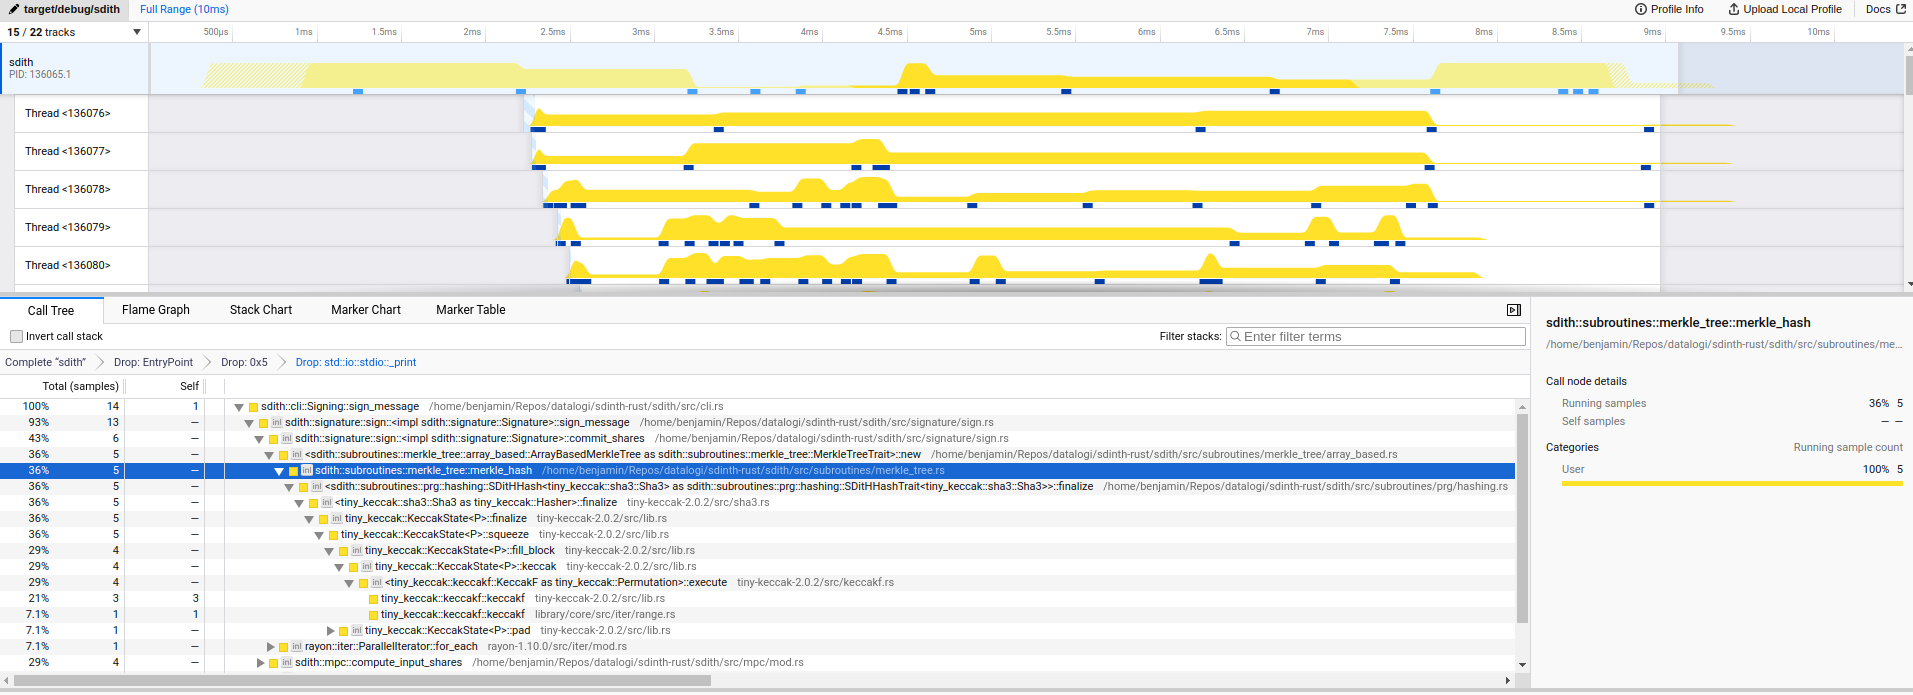
\includegraphics[width=\textwidth]{images/samply.png}
  \caption{Samply Profiler HTML Output}
  \label{fig:samply}
\end{figure}

\subsection{Build Configuration}

Rust has a number of configurations that you can apply to the compiler when building a project. These are easily configured using \textit{profiles} in the \texttt{Cargo.toml} file. We configured our optimised release profile as follows:

\begin{minted}{toml}
  [profile.release]
  strip = "debuginfo"
  codegen-units = 1  
  lto = "fat"        
  opt-level = 3      
  panic = "abort"
\end{minted}

The release profile was configured to maximize optimization during the compilation process. Specifically, the following settings were applied:

\begin{itemize}
  \item \mintinline{toml}{strip = "debuginfo"}: This strips debug information from the binary, reducing its size and improving performance.

  \item \mintinline{toml}{codegen-units = 1}: This disables parallel code compilation, resulting in slower compilation times. However, it often provides increased runtime performance and reduces the binary size by allowing the compiler to optimize more effectively.

  \item \mintinline{toml}{lto = "fat"}: This enables ``fat'' Link Time Optimization (LTO), which attempts to optimize across all crates within the dependency graph, enhancing overall performance by analyzing and optimizing the entire codebase.

  \item \mintinline{toml}{opt-level = 3/"z"}: This applies the highest level of performance optimizations offered by the compiler, enabling aggressive optimizations for runtime efficiency. To test the difference between optimising for binary size and performance, we ran the \textit{release} profile with both level 3 and \mintinline{toml}{"z"}, which optimises for binary size as opposed to performance.

  \item \mintinline{toml}{panic = "abort"}: This setting ensures that the program aborts immediately on a panic, without performing unwinding. If unwinding (e.g., via the \rust{catch_unwind} macro) is not required, setting \texttt{panic} to \texttt{"abort"} reduces binary size and often provides a slight performance boost.
\end{itemize}

\subsubsection{Parallelisation}
A common optimization technique in modern programming is to leverage the multi-core architecture of modern CPUs by employing \textit{parallelization} or \textit{multi-threading}. This approach allows programs to execute multiple tasks concurrently, significantly improving performance for computationally intensive operations.

In many programming languages, multi-threading support is either limited or not guaranteed, often requiring developers to rely on external libraries or frameworks. However, Rust provides robust and native support for \textit{thread-safe} parallelization. With Rust's ownership system and built-in concurrency primitives, developers can write highly performant parallel code while minimizing risks of common concurrency issues such as data races or deadlocks.

The \textit{rayon}~\cite{rayon} package implements easy-to-use data-parallelisation through their parallel iterators
\begin{minted}{rust}
  use rayon::prelude::*;
  fn sum_of_squares(input: &[i32]) -> i32 {
      input.par_iter() // <-- just change that!
          .map(|&i| i * i)
          .sum()
  }
\end{minted}

Although custom parallelization can sometimes outperform \textit{rayon}, the library provides an intuitive interface that enables parallelization with minimal effort, often requiring just a single line of modification. In this project, we have opted to use \textit{rayon} and reserved custom parallelization for the future.

\subsubsection{Single Instruction Multiple Data}
Single Instruction Multiple Data or SIMD for short, is a way to better utilize a CPU when dealing with data in the form of Vectors. It is a way for the CPU to do a single instruction but on multiple data points at the same time by splitting the data into chunks that fit into a single register. This can greatly improve performance when dealing with large amounts of data. Rust has support for SIMD through the \texttt{std::simd} module. This module provides access to a portable abstraction for SIMD operations that is not bound to any particular hardware architecture.

A simple example could be adding two vectors together:
\begin{minted}{rust}
fn simple_vector_addition() -> [f32; 4] {
    let mut x = [1.0, 2.0, 3.0, 4.0];
    let y = [4.0, 3.0, 2.0, 1.0];
    for i in 0..4 {
        x[i] += y[i];
    }
    x
}

\end{minted}

Instead of looping through the data we can use SIMD to do the operation in one go:

\begin{minted}{rust}
fn simple_simd_vector_addition() -> [f32; 4] {
    // create SIMD vectors
    let x: f32x4 = f32x4::from_array([1.0, 2.0, 3.0, 4.0]);
    let y: f32x4 = f32x4::from_array([4.0, 3.0, 2.0, 1.0]);

    // SIMD operation
    let z = x + y; // z = [5.0, 5.0, 5.0, 5.0]
    z.to_array() 
}
\end{minted}

In our implementation, we utilize \texttt{std::simd} from Rust's \textit{nightly} version. While it would be preferable to compile with the stable version, this implementation provides largely architecture-independent SIMD support. See \href{https://github.com/rust-lang/rust/issues/86656}{the issue} on the Rust repository for more on its development.

\chapter{Specification}\label{ch:spec}

The SDitH protocol is founded on the computational hardness of the Syndrome Decoding (SD) problem for random linear codes over a finite field, as described in \autoref{sec:syndrome}. To recall, the problem is formally stated:
\begin{quote}
  Given a parity-check matrix $H \in \mathbb{F}_q^{(m-k) \times m}$ in standard form and a syndrome $y \in \mathbb{F}_q^{m-k}$, the challenge is to find a vector $x \in \mathbb{F}_q^m$ such that $Hx = y$ and $wt(x) \leq w$, where $wt(x)$ denotes the Hamming weight of $x$. This can be expressed as:
  \begin{align*}
    y = Hx = H'x_a + x_b, \quad \text{where } H' \in \mathbb{F}_q^{(m-k) \times k},
  \end{align*}
  with $x = (x_a \mid x_b)$ denoting the concatenation of subvectors $x_a$ and $x_b$.
\end{quote}

The SDitH protocol establishes a signature scheme by demonstrating the correctness of a public SD instance $(H, y)$ using a secret witness derived from $x$. Its construction unfolds in three main steps:
\begin{enumerate}
  \item \textbf{Defining an MPC protocol:} Define a multi-party computation (MPC) protocol that enables $N$ parties to collaboratively verify the correctness of the public SD instance $(H, y)$ using a private witness $x$.
  \item \textbf{Transforming into a ZK-PoK:} Convert the MPC protocol into a zero-knowledge proof of knowledge (ZK-PoK) through the MPC-in-the-Head (MPCitH) framework, detailed in \autoref{sec:mpcinth}.
  \item \textbf{Deriving a signature scheme:} Adapt the ZKP into a digital signature scheme using the Fiat-Shamir transformation, as described in \autoref{sec:fiatshamir}.
\end{enumerate}

The construction is highly modular, allowing flexibility and adaptability, as you can tweak the SD instance, the MPC protocol, the MPCitH and Fiat-Shamir transformations. The authors propose two distinct protocols: the \textit{hypercube} and the \textit{threshold} variant. For this report, we focus on the \textit{threshold} variant~\cite{aguilarsyndrome11,feneuil2023threshold,feneuil2023threshold2}, as it offers significant performance enhancements compared to both the initial protocol~\cite{feneuil2022syndrome} and the \textit{hypercube} variant~\cite{aguilarsyndrome11,aguilar2023return,feneuil2023threshold2} -- at the cost of slightly larger signature sizes.

This chapter presents a comprehensive specification of the SDitH Signature Scheme in the Threshold variant. The construction is based on the SDitH MPC protocol in \autoref{sec:sdith-mpc}, its transformation into ZK-PoK using MPCitH (detailed in Appendix \ref{sec:sdith-zkpok}) and finally transformation into a signature scheme in \autoref{sec:sdith-signature}. Additionally, we describe optimizations applied to the protocol, such as avoiding interpolation and utilizing the $d$-split variant of the SD instance. A detailed table summarizing the protocol parameters and security assumptions is provided in \autoref{tab:sdith-protocol-parameters}.

\begin{table}[]
  \begin{tabular}{p{0.12\textwidth}p{0.78\textwidth}}
    \hline
    \multicolumn{2}{l}{\textbf{Syndrome Decoding Parameters}}                                                                             \\
    $q$                          & Size of the SD base field.                                                                             \\
    $m$                          & Code length.                                                                                           \\
    $k$                          & Vector dimension.                                                                                      \\
    $w$                          & Hamming weight bound.                                                                                  \\
    $d$                          & Parameter of the $d$-splitting variant.                                                                \\ \hline

    \multicolumn{2}{l}{\textbf{Signature Parameters}}                                                                                     \\
    $\lambda$                    & Security parameter.                                                                                    \\
    $N$                          & Number of secret parties.                                                                              \\
    $\tau$                       & Number of repetitions.                                                                                 \\
    $t$                          & Number of random evaluation points.                                                                    \\ \hline

    \multicolumn{2}{l}{\textbf{Syndrome Decoding Instance}}                                                                               \\
    $H$                          & Parity-check matrix.                                                                                   \\
    $x$                          & Solution of the SD instance satisfying $wt(x) \leq w$.                                                 \\
    $y$                          & Syndrome computed as $y = Hx$.                                                                         \\
    $H'$                         & Random part of the parity-check matrix such that $H = (H' \mid I_{m-k})$.                              \\
    $(x_A, x_B)$                 & Two halves of the SD solution satisfying $y = H' x_A + x_B$.                                           \\ \hline

    \multicolumn{2}{l}{\textbf{Fields}}                                                                                                   \\
    $\mathbb{F}_q$               & Field with $q$ elements: base field of the SD instance.                                                \\
    $f_1, \ldots, f_q$           & Elements of $\mathbb{F}_q$.                                                                            \\
    $\mathbb{F}_{\text{points}}$ & Extension field of $\mathbb{F}_q$ (base field of the MPC elements $\alpha, \beta, v, r, \varepsilon$). \\
    $\eta$                       & Field extension such that $\mathbb{F}_{\text{points}} = \mathbb{F}_q^\eta$.                            \\ \hline

    \multicolumn{2}{l}{\textbf{Multi-Party Computation}}                                                                                  \\
    $S, Q, P$                    & Polynomials in $\mathbb{F}_q[X]$, witnesses for the syndrome decoding proof.                           \\
    $F$                          & Vanishing polynomial of the set $\{f_1, \ldots, f_m\} \subseteq \mathbb{F}_q$                          \\
    $a, b, c$                    & Beaver triple satisfying $a_k \cdot b_k = c_k$, $\forall k \in [1 : t]$.                               \\
    $\alpha, \beta, v$           & Broadcast values (coordinates in $\mathbb{F}_{\text{points}}$).                                        \\
    $i$                          & Index of a party in $[1 : N]$.                                                                         \\
    $\sh{v}$                     & Sharing of a value $v$.                                                                                \\
    $p$                          & False positive probability of the MPC protocol.                                                        \\
    $\ell$                       & Privacy threshold (number of open parties).                                                            \\
    $I$                          & Set of open parties $(I \subseteq [1 : N], |I| = \ell)$.                                               \\
  \end{tabular}
  \caption{SDitH protocol parameters overview~\cite[Table 1]{aguilarsyndrome11}.}\label{tab:sdith-protocol-parameters}
\end{table}

\section{The MPC Protocol}\label{sec:sdith-mpc}

The SDitH protocol builds upon the \textit{Multi-Party Computation in the Head} (MPCitH) framework. As a first step, we describe the underlying MPC protocol, which is used to verify the polynomial relation of the SD instance as detailed in \autoref{sec:polynomial_representation}:
\begin{align*}
  S \cdot Q = P \cdot F, \quad \text{where } S, Q, P, F \in \mathbb{F}_q[X].
\end{align*}

The foundations for secret sharing and multi-party computation (MPC) are presented in \autoref{sec:additive-sss} and \autoref{sec:mpc}, respectively. The SDitH MPC protocol is constructed using the sacrificing protocol introduced by Baum and Nof~\cite{baum2020concretely}, as detailed in \autoref{sec:mpc_sacrificing}.

Recall, that instead of sharing $x_A$, we tweak the SD instance to share $s_A$ instead allowing us to skip interpolation detailed in \autoref{sec:syndrome-avoid-interpolation}.

\begin{protocol}[SDitH MPC protocol]\label{def:sdith-mpc}
  Assume the existence of a \textit{random oracle} $R$ and a $(N-2)$-\textit{private secret sharing scheme}. Given a public SD instance $(H, y)$, and the private sharings for each party $(\sh{s_A}, \sh{P}, \sh{Q}) \in F_q$, as well as $t$ sharings of random Beaver triples $\sh{a}, \sh{b}, \sh{c} \in F_{q^4}$, the protocol proceeds as follows:
  \begin{enumerate}
    \item Sample $r^j, \varepsilon^j \in_R \mathbb{F}_{q^4}^t$ uniformly at random.
    \item For each party $P_i \in [1 : N]$:
          \begin{enumerate}
            \item Set $\sh{s_B} = y - H' \sh{s_A}$ and $\sh{S} = (\sh{s_A} \mid \sh{s_B})$.\label{step:sdith-mpc-lagrange-interpolation}
            \item Locally evaluate $\sh{S(r^j)}$, $\sh{Q(r^j)}$, and $\sh{F \cdot P(r^j)}$ for all $r^j \in \mathbb{F}_{q^4}^t$.
          \end{enumerate}
    \item For all $j \in [t]$, parties verify $\sh{S(r^j)} \cdot \sh{Q(r^j)} = \sh{P \cdot F(r^j)}$ by sacrificing \\$(\sh{a^j}, \sh{b^j}, \sh{c^j})$:
          \begin{enumerate}[topsep=0pt]
            \item Parties locally compute $\sh{\alpha^j}  = \varepsilon^j \cdot \sh{Q(r^j)} + \sh{a^j}$ and $ \sh{\beta^j}  = \sh{S(r^j)} + \sh{b^j}$.
            \item Parties broadcast $\sh{\alpha^j}$ and $\sh{\beta^j}$ to publicly recompute $\alpha^j$ and $\beta^j$.
            \item Parties locally compute:
                  \begin{align*}
                    \sh{v^j} & = \varepsilon^j \cdot \sh{F \cdot P(r^j)} - \sh{c^j} + \alpha^j \cdot \sh{b^j} + \beta^j \cdot \sh{a^j} - \alpha^j \cdot \beta^j.
                  \end{align*}
            \item Parties broadcast $\sh{v^j}$ to publicly recompute $v^j$.
            \item Parties output \texttt{Accept} if $v^j = 0$, and \texttt{Reject} otherwise.
          \end{enumerate}
  \end{enumerate}
\end{protocol}
Note that the protocol requires the evaluation of a polynomial $P \in \mathbb{F}_q^{\deg(P)}$ at a point $r \in \mathbb{F}_q^\eta$, where the coefficients of $P$ lie in $\mathbb{F}_q$ and the evaluation point $r$ is in the field extension $\mathbb{F}q^\eta$. Formally, we define the polynomial evaluation as follows:
\begin{align}
  Q(r)  = \textstyle\sum_{i=0}^{|Q|} Q_i \cdot r^{i-1}  \quad Q_i \in F_q, r \in F_q^\eta\label{eq:sdith_mpc_polynomial_eval}
\end{align}
To analyze the security of the protocol, we denote $p$ as the false positive probability which quantifies the likelihood that the MPC protocol incorrectly accepts an invalid instance~\cite{feneuil2022syndrome,aguilarsyndrome11}.

Let us reason about the false positive probability of the MPC protocol. We shall denote $\Delta = |\mathbb{F}_{q^4}|$. Whenever the input is invalid, i.e. $\texttt{wt}(x) > w, P, Q$ are incorrectly built, we have that $Q \cdot S \neq P \cdot F$. The probability to have the equality for $i$ evaluations among the $t$ repetitions is
\begin{align*}
  \frac{\max_{\ell \leq m + w -1} \{ \binom{\ell}{i} \binom{\Delta - \ell}{t-i} \}}{\binom{\Delta}{t}}
\end{align*}
since $Q\cdot S - P \cdot F$ is a polynomial pf degree at most $m + w -1$. This is following \autoref{lem:schwartz}. Whenever this event occurs, the probability of a false positive is bounded by
\begin{align*}
  \left(\frac{1}{\Delta}\right)^{t-i}
\end{align*}
For the $d$-split variant, we have that each polynomial is split into chunks of degree $m/d$ and $w/d$. Therefore the probability of a false positive is bounded by \autoref{lem:sdith-mpc-soundness}.

\begin{lemma}[False positive probability $p$ of \autoref{def:sdith-mpc}]\label{lem:sdith-mpc-soundness}
  Let $x_A = \texttt{open}(\sh{x_A})$. If $x_A$ corresponds to a valid SD instance $(H', y)$ and if all sharings are correctly generated. Then \autoref{def:sdith-mpc} always outputs \texttt{Accept}. Otherwise, the probability of a false positive is bounded by
  \begin{align*}
    p = \sum_{i=0}^t \frac{\max_{\ell \leq (m + w)/d-1} \{ \binom{\ell}{i} \binom{\Delta - \ell}{t-i} \}}{\binom{\Delta}{t}} \cdot \left(\frac{1}{\Delta}\right)^{t-i}
  \end{align*} over the randomness $r$ and $\varepsilon$
\end{lemma}

\section{The Threshold Signature Protocol}\label{sec:sdith-signature}

The initial protocol for the SDitH signature scheme is seen in~\cite[Figure 1]{aguilarsyndrome11} and was first introduced in~\cite[Figure 1, p19]{feneuil2022syndrome}.

\subsubsection{Threshold variant}\label{sub:sdith-threshold-sss}

The threshold variant of the MPC protocol (\autoref{def:sdith-mpc}) is obtained by incorporating \textit{Shamir's Secret Sharing Scheme} (SSSS), as described in \autoref{sub:shamir}. By replacing the additive secret sharing scheme with Shamir's polynomial-based scheme, the protocol is extended into a $(\ell+1, N)$-threshold MPC protocol, where any $\ell+1$ out of $N$ parties can reconstruct the secret, while $\ell$ parties gain no information about the secret.

\begin{theorem}[Linear functions of \autoref{def:sdith-mpc}]\label{thm:sdith-mpc-linear}
  By the definition of the MPC protocol \autoref{def:sdith-mpc}, there exist linear functions
  \begin{align}
    \varphi^1_{r,\varepsilon}                 & : (s_A, P, Q, a, b, c) \mapsto (\alpha, \beta), \\
    \varphi^2_{r, \varepsilon, \alpha, \beta} & : (s_A, P, Q, a, b, c) \mapsto v,
  \end{align}
  such that each party locally computes $\varphi^1$ and $\varphi^2$ on the input shares $\sh{s_A}_i, \sh{P}_i, \sh{Q}_i, \sh{a}_i, \sh{b}_i, \sh{c}_i$, and randomness $r, \varepsilon$ producing $\sh{\alpha}_i, \sh{\beta}_i, \sh{v}_i$ as valid sharings of $\alpha, \beta, v$.
\end{theorem}

The authors suggest a tweak to the MPC input generation in the following way: Define the \texttt{input\_plain} as the tuple containing the MPC inputs:
\begin{align*}
  \texttt{input\_plain} = (s_A, P, Q, a, b, c)
\end{align*}

Next, compute $\ell$ uniformly random coefficients $\texttt{input\_coef} \in \mathbb{F}_q^{|\texttt{input\_plain}|}$ and compute the $i$'th sharing of the \texttt{input\_plain}:
\begin{align}\label{equation:input_sharing}
  \sh{\texttt{input\_plain}}_i = \texttt{input\_plain} + \sum_{j=1}^\ell f_i^j \cdot \texttt{input\_coef}_j
\end{align}
Where the $f_1,\dots,f_N$ denotes $N$ non-zero elements from the field $\mathbb{F}_q$.
The MPC computation is then performed directly on the \texttt{input\_plain} and its $\ell$ coefficients from the SSSS:
\begin{align*}
  \texttt{input\_plain}     & \stackrel{\varphi^1, \varphi^2}{\longrightarrow} \texttt{broad\_plain}     \\
  \texttt{input\_coef}_1    & \stackrel{\varphi^1, \varphi^2}{\longrightarrow} \texttt{broad\_coef}_1    \\
                            & \vdots                                                                     \\
  \texttt{input\_coef}_\ell & \stackrel{\varphi^1, \varphi^2}{\longrightarrow} \texttt{broad\_coef}_\ell
\end{align*}

Due to the linearity of the MPC computation, the output shares can be reconstructed by running the sharing protocol on the broadcast shares:
\begin{align}\label{equation:input_sharing_reverse}
  (\sh{\alpha}_i, \sh{\beta}_i, \sh{v}_i) = \texttt{broad\_plain} + \sum_{j=1}^\ell f_i^j \cdot \texttt{broad\_coef}_j
\end{align}

\subsubsection{PK setup}
The nature of an SD instance allows the protocol to seamlessly transform into a \textit{public-key signature scheme}. Here, the pair $(H, y)$ acts as the public key, while the solution to the SD instance $x$ serves as the private key. The keys is then expanded to $(H', y), (s_A, P, Q)$ following the transformations detailed in \autoref{sec:syndrome}. Furthermore, the public key can be optimised for communication by instead sampling $H'$ from a seed $sd_H$ making the secret key $(sd_H, y)$.

\subsubsection{ZK-PoK protocol}
First, the MPC protocol (\autoref{def:sdith-mpc}) is transformed into a ZK-PoK using the Threshold MPCitH protocols described by~\cite{feneuil2023threshold,feneuil2023threshold2}. This transformation in full lies outside the scope of this report and is deferred to Appendix \ref{sec:sdith-zkpok}. Here we leave a short overview of the transformation~\cite{aguilarsyndrome11}.

The zero-knowledge property of the protocol is guaranteed by the fact that the verifier only receives $\ell$ shares from an ($\ell + 1$)-private SSS.
The soundness of the ZK-PoK protocol relies on the binding property of the commitment scheme and the prover's inability to simulate multiple inconsistent views of the MPC protocol. By incorporating hash consistency checks and commitment verification, the ZK-PoK protocol ensures that a cheating prover cannot deviate significantly from the behavior expected in an honest execution.

\clearpage
\begin{protocol}[SDitH ZK-PoK protocol]
  \label{pro:sdith-zkpok}
  For a $(\ell + 1, N)$-threshold MPC protocol
  \begin{enumerate}[parsep=0pt, itemsep=0pt, topsep=0pt]
    \item The prover generates the input sharings and commits to the parties' shares in $h_1$
    \item The verifier challenges the prover with the randomness \(r, \varepsilon\) for the MPC protocol. This is called the \textit{MPC challenge}.
    \item The prover executes the MPC protocol (in their head) and sends the broadcast values to the verifier in $h_2$
    \item The verifier challenges the prover to open all the parties in \(I \subset [N]\) for $|I| = \ell$. This is called the \textit{viewchallenge}.
    \item The prover reveals the input shares of all the parties in \(I\).
    \item The verifier verifies the consistency of the MPC computation for the revealed parties.
  \end{enumerate}
\end{protocol}

As outlined in~\cite{feneuil2023threshold}, the general ZK-PoK (without threshold) soundness error is defined as:
\begin{align*}
  \epsilon = \frac{1}{N} + p \cdot \left(1 - \frac{1}{N}\right).
\end{align*}
By applying the threshold-based approach, the soundness error is modified and becomes:
\begin{lemma}[Soundness of \autoref{pro:sdith-zkpok}]
  The soundness error $\epsilon$ is given by:
  \begin{align*}
    \epsilon = \frac{1}{\binom{N}{\ell}} + p \cdot \frac{\ell \cdot (N - \ell)}{\ell + 1},
  \end{align*}
  where $p$ represents the false positive probability of the MPC protocol, $N$ is the total number of parties, and $\ell$ is the threshold parameter~\cite{feneuil2023threshold}.
\end{lemma}
We can see that the threshold-based approach introduces a slight degradation in the soundness of the protocol. This comes from the fact that we now require less views to be validated, which in turn increases the probability of a false positive.
To mitigate this, \textit{parallel repetition} is employed to strengthen the soundness signature protocol. Specifically, the SDitH protocol repeats the underlying ZK-PoK protocol $\tau$ times, where:
\begin{align*}
  \tau = \left\lceil \log_2\left(\frac{1}{\epsilon}\right) \cdot \lambda \right\rceil,
\end{align*}
with $\lambda$ as the security parameter and $2^{-\lambda}$ as the target soundness error~\cite{aguilarsyndrome11}. This parallel repetition reduces the overall soundness error exponentially with the number of repetitions, achieving a negligible error probability in practice.

To accommodate the repetitions, the authors incorporate a slight modification inspired by the Limbo proof system~\cite{delpech2021limbo}. Specifically, we reuse the same MPC challenges $r$ and $\varepsilon$, as well as the Beaver triples, across all $\tau$ repetitions. This tweak allows us to modify the MPC computation input so that \textit{plain broadcast} value only needs to be computed once.

\subsubsection{Fiat-Shamir transform}
Next, we apply the \textit{Fiat-Shamir heuristic} -- detailed in \autoref{sec:fiatshamir} -- to transform the challenges of the ZK-PoK protocol into a non-interactive form. This transformation is achieved by having the prover derive the challenges for MPC randomness and the opening challenge directly from the commitments of the MPC inputs and the outputs of the MPC computation in the hashes $h_1, h_2$ computed with secure hash functions~\autoref{sec:prelim_hash}.
\begin{align}
  h_n = \texttt{Hash}_n(d) \rightarrow \texttt{Hash}(n || d)\label{eq:fiatshamirhash}
\end{align}

Additionally, we incorporate the message into the second hash, enabling the pre-computation of the first part of the signature independently of the message. This optimization enhances efficiency by allowing some computations to be performed beforehand.

Finally, we introduce a $\texttt{salt} \in \{0,1\}^{2\lambda}$, which serves as pseudo-randomness for commitments and seed generation. The use of a $\texttt{salt}$ ensures that the protocol remains secure and avoids reliance on externally provided randomness.

\subsubsection{Optimizing Signature Size and Verification}\label{sec:mpc_thresh_tweak}
In the original SDitH protocol~\cite[Figure 1]{aguilarsyndrome11} -- without threshold SSS -- the signature includes both hashes $h_1, h_2$ and all input shares in $I$, where $|I| = N - 1$.
To verify the signature, the verifier recomputes the commitments for each share in $I$, and along with the last missing commitment $\texttt{com}_i$ for $i \notin I$, reconstructs $h_1$. The verifier then executes the MPC protocol for the opened shares and recomputes $h_2$ from the resulting output shares. We will now go over some of the techniques applied to optimize the signature size and verification process.

\begin{theorem}[Sharing Redundancy of Shamir's Secret Sharing Scheme]
  The full set of broadcast shares $\sh{\alpha}_i, \sh{\beta}_i, \sh{v}_i$ for $i \in N$ can be deduced from $\ell + 1$ broadcast shares. That is, the full sharing forms a Reed-Solomon code word.
\end{theorem}

\noindent
For the threshold variant, however, we can optimize this process by selecting a predefined set
\begin{align*}
  \mathcal{E} = \{\sh{\alpha}_i, \sh{\beta}_i, \sh{v}_i\}_{i \in E},
\end{align*}
where $E \subseteq N$ and $|E| = \ell + 1$. We then set $h_2 = \texttt{Hash}_2(\mathcal{E})$. In this case, the signature includes the input shares $\{\sh{\alpha}_i, \sh{\beta}_i, \sh{v}_i\}_{i \in I}$, plus a single broadcast share, allowing the verifier to recompute $h_2$. However, this approach requires the verifier to interpolate the sharing coefficients
\begin{align}
  \texttt{broad\_plain}, \texttt{broad\_coef}_1, \dots, \texttt{broad\_coef}_\ell.\label{eq:mpc_shamir_coeffs}
\end{align}
To avoid this interpolation, we note that $\mathcal{E}$ is fully determined by the coefficients. Therefore, we can instead use these as the input of $h_2$, enabling the signer to bypass the computation of $\mathcal{E}$. Furthermore, the signature can include \autoref{eq:mpc_shamir_coeffs} instead of $h_2$. This allows the verifier to compute $h_2$ and evaluate $\{\sh{\alpha}_i, \sh{\beta}_i, \sh{v}_i\}_{i \in I}$ directly, avoiding the need for interpolation.

Following from \autoref{thm:sdith-mpc-linear}, for every party $i$, there exists a direct linear relationship between the Beaver triple shares $\sh{a}_i, \sh{b}_i, \sh{c}_i$ and the broadcast shares $\sh{\alpha}_i, \sh{\beta}_i, \sh{v}_i$. This observation enables the removal of Beaver triples within the signature. Instead, the verifier can compute these triples directly using the shares of the witness, $(\sh{s_A}_i, \sh{P}_i, \sh{Q}_i)$, along with the broadcast shares $(\sh{\alpha}_i, \sh{\beta}_i, \sh{v}_i)$ for $i \in I$. We denote a function \textit{TruncateBeaver}
\begin{align}
  \text{TruncateBeaver} : \sh{\texttt{input}}_i = (\sh{s_A}_i, \sh{P}_i, \sh{Q}_i, \sh{a}_i, \sh{b}_i, \sh{c}_i) \mapsto (\sh{s_A}_i, \sh{P}_i, \sh{Q}_i) = \sh{\texttt{wit}}_i\label{eq:truncate_beaver}
\end{align}
This process is referred to as \textit{inverse MPC computation}.

\begin{theorem}[Inverse MPC computation]\label{thm:mpc_inverse}
  For an MPC protocol \autoref{thm:sdith-mpc-linear} we have an inverse MPC computation with two functions
  \begin{align}
    \phi^1_{r,\varepsilon}        & : (s_A, P, Q, \alpha, \beta, v) \mapsto (a, b), \\
    \phi^2_{r, \varepsilon, a, b} & : (s_A, P, Q, \alpha, \beta, v) \mapsto c,
  \end{align}

  We have that for any $(a,b,c) \stackrel{\phi^1, \phi^2}{\longleftarrow} (s_A, P, Q, \alpha, \beta, v, r, \varepsilon)$, then
  \begin{align*}
    (s_A, P, Q, a, b, c, r, \varepsilon) \stackrel{\varphi^1, \varphi^2}{\longrightarrow} (\alpha, \beta, v)
  \end{align*}
\end{theorem}

To formalize the approach, we introduce the following notations:

Denote $Q'$ as the witness polynomial $Q$ with its leading coefficient removed. Additionally, let $\sh{Q^0}$ represent the polynomial with a leading coefficient of $0$, and $\sh{Q^1}$ the polynomial with a leading coefficient of $1$.

Define two reconstructions of $S$ as:
\begin{align*}
  S_1 & = (s_A, y - H \cdot s_A), \\
  S_0 & = (s_A, H \cdot s_A).
\end{align*}

These two updates enable the inverse MPC computation by ensuring that the constant parts of the affine functions are introduced for one party and therefore not removed during the inverse MPC computation.

Therefore, we include an input parameter \texttt{with\_offset} in the MPC protocol \autoref{def:sdith-mpc}, denoted $\varphi^1_{\texttt{with\_offset}}$. This parameter determines whether $S_{\texttt{with\_offset}}, Q_{\texttt{with\_offset}}$ is used. Similarly, $\varphi^2_{\texttt{with\_offset}}$ indicates whether the constant derived from the plain outputs, $-\alpha \cdot \beta$, is added to $v$.

The same applies to $\phi^1$ and $\phi^2$ for the inverse MPC computation. For further clarity, a \textit{toy example} illustrating the inverse MPC computation is provided in Appendix \ref{app:toy_example}.

\subsubsection{The protocols}
We introduce the signing and verification protocols in \autoref{def:sdith-sign} and \autoref{def:sdith-verify}, respectively.

\begin{protocol}[SDitH Signing Protocol]\label{def:sdith-sign}
  \setlength{\parindent}{0pt}
  \setlength{\parskip}{5pt}
  \titlespacing*{\paragraph}{0pt}{1pt}{1em}
  Given a public key (SD instance) $pk = (H, y)$, secret key (SD solution) $sk = (s_A, Q, P)$, message $m \in \{0,1\}^*$ and security parameters $\lambda, \tau$

  \paragraph{Assumptions}

  \begin{itemize}[itemsep=0pt, topsep=0pt, parsep=0pt]
    \item $(\ell + 1, N)$-threshold MPC protocol $\varphi^1, \varphi^2$ (\autoref{def:sdith-mpc}, \autoref{sec:mpc}), \autoref{equation:input_sharing}
    \item Merkle Tree Commitment Scheme: \texttt{MerkleTree} and \texttt{MerkleAuthPath} (\autoref{sub:merkle_tree_prelim})
    \item Collision Resistant hash functions $\texttt{Hash}_n$ (\autoref{eq:fiatshamirhash})
    \item Random oracle $\texttt{PRG}$ (\autoref{sec:prelim_hash})
    \item Extendable output hash function \texttt{XOF} (\autoref{sec:xof})
  \end{itemize}

  \paragraph{Setup} Initialise entropy

  \begin{enumerate}[itemsep=0pt, topsep=0pt, parsep=0pt]
    \item Sample a random salt: $\texttt{salt} \leftarrow \{0, 1\}^{2\lambda}$.
    \item Sample a root seed: $sd \leftarrow \{0, 1\}^{\lambda}$.
    \item Initialise \texttt{XOF} from $sd$, \texttt{salt}
  \end{enumerate}
  \paragraph{Phase 1} Prepare the MPCitH inputs.

  \begin{enumerate}[itemsep=0pt, topsep=0pt, parsep=0pt]
    \item Compute Beaver triples $\mathcal{B} = a^{j}, b^{j}, c^{j}$ for all $j \in t$ and construct $\texttt{input\_plain} = (sk, \mathcal{B})$
    \item For each iteration $e \in [\tau]$
          \begin{enumerate}[itemsep=0pt, topsep=2pt, parsep=0pt]
            \item compute $\texttt{input\_coef}_j^e \leftarrow \texttt{XOF}$ for each $j \in \ell$
            \item compute input shares for $i \in [N]$
                  \begin{align*}
                    \sh{\texttt{input\_plain}}_i^e =
                    \begin{cases}
                      \texttt{input\_coef}^e_{\ell}                                                & \quad i = 1 \\
                      \texttt{input\_plain} + \sum_{j=1}^\ell f_i^j \cdot \texttt{input\_coef}_j^e & \quad i > 1
                    \end{cases}
                  \end{align*}
            \item compute commitments for $i \in [N]$
                  \begin{align*}
                    \texttt{com}_i^{e} := \texttt{Hash}_0(\texttt{salt}, e, i, \sh{\texttt{input\_plain}}_i^e)
                  \end{align*}
            \item compute the Merkle commitment
                  \begin{align*}
                    \texttt{root}^{e} = \texttt{MerkleTree}(\texttt{com}_1^{e}, \ldots, \texttt{com}_N^{e})
                  \end{align*}
          \end{enumerate}
  \end{enumerate}

  \paragraph{Phase 2} Compute first challenge (\textit{MPC challenge})
  \begin{enumerate}[itemsep=0pt, topsep=0pt, parsep=0pt]
    \item Compute the first hash
          \begin{align*}
            h_1 = \texttt{Hash}_1(pk, \texttt{salt}, \texttt{root}^{1}, \ldots, \texttt{root}^{\tau})
          \end{align*}
    \item Generate first challenge (MPC randomness)
          \begin{align*}
            r, \varepsilon \leftarrow \texttt{PRG}(h_1)
          \end{align*}
  \end{enumerate}

  \paragraph{Phase 3} Simulation of the MPC Protocol.
  \begin{enumerate}[itemsep=0pt, topsep=0pt, parsep=0pt]
    \item Compute plain broadcast $\texttt{broad\_plain} \stackrel{\varphi^1_1}{\longleftarrow} \texttt{input\_plain}, r, \varepsilon$\footnote{$\varphi^2$ is skipped as $v = 0$ for an honest execution.}
    \item For $e \in [\tau]$, compute broadcast shares
          \begin{align*}
            \texttt{broad\_coef}_j^e \stackrel{\varphi^1_0, \varphi^2_0}{\longleftarrow} \texttt{input\_coef}_j^e, r, \varepsilon \quad \text{for each } j \in \ell
          \end{align*}
  \end{enumerate}

  \paragraph{Phase 4} Compute second challenge (\textit{View opening challenge})
  \begin{enumerate}[itemsep=0pt, topsep=0pt, parsep=0pt]
    \item Compute the second hash
          \begin{align*}
            h_2 = \texttt{Hash}_2(m, \texttt{salt}, h_1, \texttt{broad\_plain}, \{\texttt{broad\_coef}^e_1, \dots, \texttt{broad\_coef}^e_\ell\}_{e=1}^\tau)
          \end{align*}
    \item Compute the second challenge set $I \subset [1:N] \leftarrow \texttt{PRG}(h_2)$ for $|I| = \ell$
  \end{enumerate}

  \paragraph{Phase 5} Building of the signature output the signature $\sigma$ for $e \in [\tau]$ and $i \in I$
  \begin{enumerate}[itemsep=0pt, topsep=0pt, parsep=0pt]
    \item Compute authentication paths
          \begin{align*}
            \texttt{auth}^e = \texttt{MerkleAuthPath}(\{\texttt{com}^e_i\}_{i \in I})
          \end{align*}
    \item Compute witness shares
          \begin{align*}
            \sh{\texttt{wit}}_i^e = \text{TruncateBeaver}(\texttt{input}^e_i)
          \end{align*}
    \item Build the signature
          \begin{align*}
            \sigma = & \ (\ m \mid \texttt{salt} \mid h_1                                \\
                     & \mid \texttt{broad\_plain}                                        \\
                     & \mid \texttt{broad\_coef}^e_1, \dots, \texttt{broad\_coef}^e_\ell \\
                     & \mid \texttt{auth}^e                                              \\
                     & \mid \sh{\texttt{wit}}_i^e                                        \\
                     & \mid I\ )
          \end{align*}
  \end{enumerate}
\end{protocol}

\begin{protocol}[SDitH Verification Protocol]\label{def:sdith-verify}
  \setlength{\parindent}{0pt}
  \setlength{\parskip}{5pt}
  \titlespacing*{\paragraph}{0pt}{1pt}{1em}
  Given a public SD instance $pk = (H, y)$, security parameters $\lambda, \tau$, and a signature
  \begin{align*}
    \sigma = & \ (\ m \mid \texttt{salt} \mid h_1                                \\
             & \mid \texttt{broad\_plain}                                        \\
             & \mid \texttt{broad\_coef}^e_1, \dots, \texttt{broad\_coef}^e_\ell \\
             & \mid \texttt{auth}^e                                              \\
             & \mid \sh{\texttt{wit}}_i^e                                        \\
             & \mid I\ )
  \end{align*}

  \paragraph{Assumptions}
  \begin{enumerate}[itemsep=0pt, topsep=0pt, parsep=0pt]
    \item $(\ell + 1, N)$-threshold MPC protocol with inverse computation $\phi^1, \phi^2$ (\autoref{def:sdith-mpc}, \autoref{thm:mpc_inverse}, \autoref{sec:mpc}), \autoref{equation:input_sharing_reverse}
    \item Merkle Tree Commitment Scheme: \texttt{MerkleRootFromAuthPath} (\autoref{sub:merkle_tree_prelim})
    \item Collision resistant  hash functions $\texttt{Hash}_n$ (\autoref{eq:fiatshamirhash})
    \item Random oracle $\texttt{PRG}$ (\autoref{sec:prelim_hash})
    \item Extendable output hash function \texttt{XOF} (\autoref{sec:xof})
  \end{enumerate}

  \paragraph{Protocol} The protocol proceeds as follows for $e \in [\tau]$ and $i \in I$:
  \begin{enumerate}[itemsep=0pt, topsep=0pt, parsep=0pt]
    \item Recompute the first challenge $r, \varepsilon \leftarrow \texttt{PRG}(h_1)$
    \item Compute broadcast shares
          \begin{align*}
            \mathcal{B'}_i = \sh{\alpha^e}_i, \sh{\beta^e}_i, \sh{v^e}_i =
            \begin{cases}
              \texttt{broad\_coef}^e_\ell                                                  & \quad i = 1 \\
              \texttt{broad\_plain} + \sum_{j=1}^\ell f_i^j \cdot \texttt{broad\_coef}_j^e & \quad i > 1
            \end{cases}
          \end{align*}
    \item Recompute Beaver triples
          \begin{align*}
            \sh{a}_i, \sh{b}_i, \sh{c}_i \stackrel{\phi^1_{i > 1}, \phi^2_{i > 1}}{\longleftarrow} pk, \texttt{broad\_plain}, \sh{\texttt{wit}}_i^e, \mathcal{B'}_i, r, \varepsilon
          \end{align*}
          Set $\texttt{input}^e_i = (\texttt{wit}_i^e, \mathcal{B'}_i)$
    \item Recompute commitments
          \begin{align*}
            \texttt{com}^e_i = \texttt{Hash}_0(\texttt{salt}, e, i, \sh{\texttt{input}^e_i})
          \end{align*}
    \item Recompute Merkle tree roots
          \begin{align*}
            \texttt{root}^e = \texttt{MerkleAuthPath}(\texttt{auth}^e,\{\texttt{com}^e_i\}_{i \in I})
          \end{align*}
    \item Recompute $\tilde{h_1} = \texttt{Hash}_1(pk, \texttt{salt}, \texttt{root}^e, \ldots, \texttt{root}^{\tau})$
  \end{enumerate}

  Output \texttt{Accept} if and only if $h_1 \stackrel{?}{=} \tilde{h_1}$, and \texttt{Reject} otherwise.

\end{protocol}

\subsection{Key and Signature sizes}

The SDitH signature scheme has the following memory performances

\subsubsection{Public key}
The public key $pk = (\texttt{seed\_H}, y)$ consists of the seed of length $\lambda$ to generate the matrix $H'$ and the public output of $y \in \mathbb{F}_q^{m-k}$.
\begin{align*}
  |pk| = \lambda / 8 + (n - k) \text{ bytes}
\end{align*}

\subsubsection{Secret key}
The secret key $sk = (\texttt{seed\_H}, y, s_A, P, Q)$ consists of the public key and the solution to the syndrome decoding problem: $s_A$, and the polynomials $P$ and $Q$, all derivied from the solution $x$.
\begin{align*}
  |sk| = |pk| + k + 2w = \lambda/8 + n + 2w \text{ bytes}
\end{align*}
Note that you could set the secret key to be some $\texttt{seed}_{root}$ and then compute the SD instance and solution at signing time. However, this would add the key generation time to the signing time, but would allow for a secret key of size $\lambda/8$ bytes.
\subsubsection{Signature}
\begin{align*}
  \text{Total Size} =
   & \ 2\lambda \quad                                                                 &  & \rightarrow \text{size of the salt}                               \\
   & + 2\lambda \quad                                                                 &  & \rightarrow \text{size of } h_1                                   \\
   & + 2d \cdot t \cdot \log_2(|F_{\text{points}}|) \quad                             &  & \rightarrow \text{size of broad plain}                            \\
   & + \tau \cdot \ell \cdot (k \cdot \log_2(|F_q|) + 2w \cdot \log_2(|F_q|)) \quad   &  & \rightarrow \text{size of } (\text{wit share}[e][i])_{i \in I[e]} \\
   & + \tau \cdot \ell \cdot (2d + 1) \cdot t \cdot \log_2(|F_{\text{points}}|) \quad &  & \rightarrow \text{size of broad share}                            \\
   & + \tau \cdot \ell \cdot 2\lambda \cdot \log_2(N / \ell) \quad                    &  & \rightarrow \text{size of } \text{auth}[e].
\end{align*}

Assuming that each field element in $F_q$ is represented by a byte, the signature size (in bytes) is given by:
\begin{align*}
  |\sigma| =
  \lambda + 2d \cdot t \cdot \eta + \tau \cdot \ell \cdot k + 2w + (2d + 1) \cdot t \cdot \eta + \log_2(N / \ell).
\end{align*}

For each of the NIST categories the keys and signature sizes are presented in \autoref{tab:secparam}.

\begin{table}[H]
  \centering
  \begin{tabular}{|l|r|r|r|}
    \hline
                      & \multicolumn{3}{c}{\textbf{Sizes (in bytes)}}                                \\
    \textbf{Category} & Public key                                    & Secret key & Signature (Max) \\
    \hline
    I                 & $132$                                         & $432$      & $10684$         \\
    III               & $180$                                         & $628$      & $25964$         \\
    V                 & $244$                                         & $838$      & $45676$         \\
    \hline
  \end{tabular}
  \caption{Sizes (in bytes) for the categories in the SDitH protocol.}
  \label{tab:sizes}
\end{table}

\section{Security}

The security analysis of the SDitH signature scheme is based on the proposed standardization requirements from the 2022 NIST call for proposals of non-lattice based signature schemes~\cite{nistcall}. Therefore, as a preliminary, we will describe the reasoning and requirements of the NIST standardization process.

With the development of new quantum algorithms and unknowns in the capacities of the future quantum computers, there remain large uncertainties in estimating the security of the algorithms. To combat these uncertainties, NIST proposed for the 2022 stadardization effort, to define the security of submissions in a range of five categories. Each, with an easy-to-analyze cryptographic primitive providing the lower bound for a variety of metrics deemed relevant to practical security.

\begin{definition}\label{def:nistsec}
  Any attack that breaks the relevant security definition must require computational resources comparable to or greater than those required for key search on a block cipher with a 128-bit (e.g. AES-128), 192-bit (e.g. AES-192) and 256-bit (e.g. AES-256) for categories \textbf{I}, \textbf{III} and \textbf{V} respectively.
\end{definition}

In terms of quantum security, the complexity and capability of quantum algorithms are measured in terms of quantum circuit size, i.e. the number of quantum gates in the quantum circuit. In order to estimate the quantum security of the signature protocols, circuit size can be compared to the resources required to break the security of \autoref{def:nistsec}.

\subsubsection{NIST Categories}

The SDitH specification provides security parameters adhering to categories I, III and V. Therefore, according to the proposal by NIST, the SDitH specification provides security metrics in terms of quantum circuit depth to optimal key recovery for AES-128, AES-192 and AES-256 for categories \textbf{I}, \textbf{III} and \textbf{V} respectively. These are estimated to be $2^{143}$, $2^{207}$ and $2^{272}$ classical gates~\cite{nistcall}.

\subsubsection{Security Assumptions}

The SDitH protocol is secure under the following assumptions:

Syndrome Decoding instances cannot be solved in complexity lower than $2^\kappa$ corresponding to the complexity of breaking AES by exhaustive search (see \autoref{def:nistsec}) in terms of quantum circuit size. For this, $\kappa$ is defined as $143$, $207$ and $272$ for the categories~\cite{nistcall}. Furthermore, the XOF primitive used is secure with 128-bit, 192-bit, 256-bit security levels for each of the categories respectively. Finally, the Hash function used \textit{behaves as a random oracle}. Specifically, security holds in Random Oracle Model (ROM) and Quantum Random Oracle Model (QROM)~\cite{aguilarsyndrome11} -- see \autoref{sub:qrom}.

\subsubsection{Security Definition}

Furthermore, the SDitH signature scheme ensures \textbf{E}xistential \textbf{U}nforgeability under \textbf{C}hosen \textbf{M}essage \textbf{A}ttack (EUF-CMA), a key security property evaluated by NIST~\cite{nistcall,aguilarsyndrome11}. In the EUF-CMA game, a challenger generates a key pair $(pk, sk)$ and provides $pk$ to the adversary, who can query a signing oracle for up to $2^{64}$ chosen messages $(m_1, \dots, m_r)$, receiving corresponding valid signatures $(\sigma_1, \dots, \sigma_r)$. The adversary wins if it produces a valid signature $(m^*, \sigma^*)$ for a message $m^*$ not queried to the signing oracle.

\subsubsection{Signature Forgery Attack}

We analyze the generic forgery attack on Fiat-Shamir transformed signature protocols as described by~\cite{kales2020attack}. This attack seeks to minimize the effective cost of a forgery attempt. For the threshold-based SDitH protocol, the adversary can choose between two strategies:
\begin{enumerate}
  \item \label{item:guessing-mpc-challenge} Guessing the unique MPC challenge.
  \item \label{item:guessing-view-challenge} Guessing the view-opening challenges for each of the $\tau$ executions.
\end{enumerate}

In strategy~\ref*{item:guessing-mpc-challenge}, the adversary attempts to exploit false positives in the MPC protocol. This is lower bounded by the cost of obtaining a false positive for one truncated input share (see \autoref{eq:truncate_beaver}) in one of the $\tau$ executions, where the share is encoded by a subset $I \subset [N]$:
\begin{align*}
  \frac{1}{1 - (1-p)^{\tau \cdot \binom{N}{\ell + 1}}}.
\end{align*}

Due to the tweak in MPC input generation detailed in \autoref{sub:sdith-threshold-sss}, the adversary cannot use invalid shares to reduce the cost in strategy~\ref*{item:guessing-view-challenge}, as any such inconsistency will be detected by the verifier. Thus, the cost of this strategy corresponds to plain guessing:
\begin{align*}
  \binom{N}{\ell}^\tau.
\end{align*}

Therefore, the total cost of a forgery attack is the maximum of the two strategies:
\begin{align}
  \max \left\{ \frac{1}{1 - (1-p)^{\tau \cdot \binom{N}{\ell + 1}}}, \binom{N}{\ell}^\tau \right\}\label{eq:forgery_attack_cost}
\end{align}

\subsubsection{Attacks against the SD problem}

The general syndrome decoding problem \autoref{def:syndrome} is a known \textbf{NP}-hard problem. The most well performing attacks are of the family \textit{Information-Set Decoding} (ISD)~\cite{aguilarsyndrome11,prange1962use}. An information-set decoding algorithm iteratively selects a set $I$ of $k$ indices (the information set) and defines $J = [1, \ldots, m] \setminus I$. A step is successful if the submatrix $H_J$ is invertible and the support of $x$ lies entirely in $J$, allowing $x$ to be computed as $x_J = H_J^{-1} y$, with other entries set to $0$. Successive work by~\cite{stern1989method,peters2009information} gives the following bounds for the complexity of an ISD algorithm. The cost of each iteration is
\begin{align}
  \begin{split}
    & C_{iter} =                                                                                  \\
    & \frac{1}{2}(n-k)^2(n+k) + \left(\left(\frac{k}{2} - p + 1\right) +
    \left(\binom{\lfloor k/2 \rfloor}{p} + \binom{k - \lfloor k / 2 \rfloor}{p}\right)(q-1)^p\right) \ell \\
    & + \frac{q}{q-1}(w-2p+1) 2p \left(1 + \frac{q-2}{q-1}\right)
    \frac{\binom{\lfloor k/2 \rfloor}{p} + \binom{k - \lfloor k / 2 \rfloor}{p}(q-1)^{2p}}{q^\ell},
  \end{split}
\end{align}
while the success probability for each iteration is
\begin{align}
  p_{succ} \binom{\left\lfloor k/2 \right\rfloor }{p} \binom{k -\left\lfloor k/2 \right\rfloor }{p} \binom{n-k-\ell}{w-2p} / \binom{n}{w},
\end{align}
and a total cost for the ISD algorithm is
\begin{align}
  \frac{C_{iter} \cdot \log_2(q)}{p_{succ}}\label{eq:sd_cost}
\end{align}

\subsubsection{$d$-split Syndrome Decoding Problem}

Categories three and five rely on a variant of the syndrome decoding problem, referred to as the \textit{$d$-split syndrome decoding problem}. This variant introduces the splitting parameter $d$, which partitions the witness $x$ into $d$ chunks:
\begin{align*}
  x & = x_1 \| \dots \| x_d \in \mathbb{F}_q^{m/d} \quad \text{wt}(x_j) = w/d
\end{align*}
In this formulation, the MPC protocol is executed $d$ times in parallel. Consequently, the polynomial relations $Q$, $P$, $S$, and $F$ are divided into $d$ corresponding polynomials, e.g.,
\begin{align*}
  \textbf{Q} & = Q_1, \dots, Q_d.
\end{align*}
Similarly, the Beaver triples $a$ and $b$ are adjusted for the $d$-split as follows:
\begin{align*}
  c_j & = \sum_{i=1}^d a_{i,j} \cdot b_{i,j}, \quad j \in [\tau].
\end{align*}
While the $d$-split variant introduces a slight reduction in security compared to the standard SD problem, this is mitigated by a small increase in the security parameters $m$, and $w$. The primary advantage of this variant lies in its flexibility. We have a bound on the size of the $|\mathbb{F}_q| \geq m/d$. Therefore, the main benefit of introducing the $d$-split version is to let the protocol work on polynomials of smaller degree and/or on specific fields which provides better performance trade-offs~\cite{aguilarsyndrome11}. The increase in parameters are given by
\begin{align}
  \epsilon_1 \geq \frac{\binom{m/d}{w/d}}{\binom{m}{w}} \cdot \epsilon_d\label{eq:d_split_epsilon}
\end{align}
a proof of this can be found in~\cite[p27]{feneuil2022syndrome}

\subsection{SDitH Parameters}

All parameters provided in \autoref{tab:secparam} and cryptographic primitives in \autoref{tab:hashparam}.

\begin{table}[H]
  \centering
  \def\arraystretch{1.5}%  1 is the default, change whatever you need
  \begin{tabular}{cccccccccccccc}
    \specialrule{.1em}{.05em}{.05em}
    \multicolumn{2}{c}{\textbf{NIST security}} &      & \multicolumn{5}{c}{\textbf{SD parameters}} &     & \multicolumn{5}{c}{\textbf{MPCitH Parameters}}                                                             \\ \cline{1-2} \cline{4-8} \cline{10-14}
    Category                                   & Bits &                                            & $q$ & $m$                                            & $k$ & $w$ & $d$ &  & N   & $\ell$ & $\tau$ & $\eta$ & $t$ \\ \hline
    \textbf{I}                                 & 143  & \textit{}                                  & 256 & 242                                            & 126 & 87  & 1   &  & $q$ & 3      & 17     & 4      & 7   \\
    \textbf{III}                               & 207  &                                            & 256 & 376                                            & 220 & 114 & 2   &  & $q$ & 3      & 26     & 4      & 10  \\
    \textbf{V}                                 & 272  &                                            & 256 & 494                                            & 282 & 156 & 2   &  & $q$ & 3      & 34     & 4      & 13  \\ \specialrule{.1em}{.05em}{.05em}
  \end{tabular}
  \caption{Security parameters for the SDitH protocol for categories one, three and five~\cite{aguilarsyndrome11}.}\label{tab:secparam}
\end{table}

\begin{table}[H]
  \centering
  \def\arraystretch{1.5}%  1 is the default, change whatever you need
  \begin{tabular}{clll}
    \specialrule{.1em}{.05em}{.05em}
         & \multicolumn{1}{c}{\textbf{I}} & \multicolumn{1}{c}{\textbf{III}} & \multicolumn{1}{c}{\textbf{V}} \\ \cline{2-4}
    Hash & SHA3-256                       & SHA3-384                         & SHA3-512                       \\
    XOF  & SHAKE-128                      & SHAKE-256                        & SHAKE-256                      \\ \specialrule{.1em}{.05em}{.05em}
  \end{tabular}
  \caption{Hash and XOF functions used in the SDitH protocol for categories one, three and five~\cite{aguilarsyndrome11}.}\label{tab:hashparam}
\end{table}

\subsubsection{SD Parameters}

The SD parameters are are calculated to ensure that known attacks like ISD \autoref{eq:sd_cost} have a complexity of at least $2^\kappa$. The field $q$ is chosen due to the fact that it is both convenient to sample, efficient on most architectures and because it yields close to optimal signature sizes~\cite{aguilarsyndrome11}. The splitting parameter $d$ is used to ensure that $m/d \leq q$ for the public $F$ polynomial of degree $m$.

\subsubsection{MPCitH Parameters}

For the MPCitH parameters, $N$ is set to the $q$ which is the maximal according to the field size. $\ell$ is set to $3$ as it provides a good trade-off between signature size and computational overhead~\cite{aguilarsyndrome11}. The parameters $t, \tau$ are given by \autoref{eq:forgery_attack_cost} and \autoref{eq:d_split_epsilon}.



%%%%%%%%%%%%%%%%%%%%%%%%%%%%%%%%%%%%%%%%%%%%%%%%%%%%%%%%%%%%%%%%%%%%%%%

\chapter{Implementation}\label{ch:impl}

We set out to implement the SDitH Protocol using a modern, well-maintained language that provides the necessary performance and security for a post-quantum secure signature scheme. To achieve this, we selected Rust~\cite{rustlangRustProgramming,nistsaferlanguages,lurklurkEffectiveRust,rustlangPerformanceBook} as the programming language. To manage the protocol efficiently, we chose to rely as little as possible on external packages and to write most of the subroutines ourselves. This included implementing subroutines for Galois Finite Fields and Merkle Tree Commitment Schemes.

For cryptographic primitives like hash functions~\cite{blakethree,tinykeccak}, we used external libraries. This is a common approach since securely developing cryptographic primitives requires significant effort and is often treated as a standalone project. Furthermore, for developing the CLI we used the \href{https://docs.rs/clap/latest/clap/}{\texttt{clap}} crate which provides a simple and intuitive API for building command line interfaces.

Initially, we aimed to base our implementation solely on the specification. However, this approach proved challenging due to ambiguities in some of the definitions, making it unclear how certain elements should be implemented and making testing the outcomes hard. To address this, we instead aligned our implementation in terms of outputs with the reference implementation. This provided a valuable tool for debugging and figuring out these ambiguities.

This section provides a detailed overview of our implementation. We present a brief walkthrough of the structure and each module in our implementation, detailing how the code aligns with the SDitH specification. Additionally, we describe the steps taken to test and optimize these modules and discuss the challenges encountered during their development.

\section{Structure}
To maintain a clear separation of concerns, we have structured the codebase using Rust modules (\autoref{sub:rust_modules}), ensuring that each component of the protocol is well-organized.

\begin{itemize}[itemsep=2pt, parsep=0pt]
  \item \texttt{Cargo.toml}: Defines the package metadata and its dependencies.
  \item \texttt{build.rs}: Specifies build steps that are executed before compiling the binary. These mostly include adding warnings on the configuration used for the build -- e.g., NIST category, optimisations enabled etc.
  \item \texttt{README.md}: Provides instructions and information for running the project. Any reader who is interested to run or develop with the code base are encouraged to read this file along with our \href{https://mactherobot.github.io/sdith-rust}{documentation}.
  \item \texttt{bencher.py}: Python script to run a collection of benchmarks.
\end{itemize}

In addition to these files, the directory includes several subdirectories:

\begin{itemize}[itemsep=2pt, parsep=0pt]
  \item \texttt{benches}, \texttt{examples}: Contains functionality for benchmarking the code. The \texttt{examples} was used to host \textit{dudect} implementation.
  \item \texttt{src}: Hosts the main codebase, structured into several submodules for modularity and clarity.
\end{itemize}

Within the \texttt{src} directory, the code is further divided into submodules, each serving a distinct purpose. We aimed to align the modules as closely as possible with their theoretical counterparts described in this report and the specification.

This modular design ensures that each aspect of the protocol is encapsulated within its respective submodule, making the codebase easier to understand, maintain, and extend.

\begin{itemize}[itemsep=2pt, parsep=0pt]
  \item \texttt{lib.rs}: Entry for the \texttt{rsdith} crate.
  \item \texttt{bin}: Binary targets for the project. Including the CLI tool and a profiling binary. Details are specified in the \texttt{README.md}.
  \item \texttt{constants}: Defines parameters and types used throughout the protocol.
  \item \texttt{kat}: Contains Known Answer Tests (KAT) for verifying implementation correctness against the reference implementation. Only included with the feature flag \texttt{kat}.
  \item \texttt{signature}: Implements the signature and verification protocols.
  \item \texttt{subroutines}: Subroutine functions supporting various components of the protocol.
        \begin{itemize}[itemsep=2pt, parsep=0pt]
          \item \texttt{arith}: Contains arithmetic operations for finite fields. Currently only has GF256 implementation.
          \item \texttt{merkle\_tree}: Implements a Merkle tree commitment scheme
          \item \texttt{prg}: Implements a pseudo-random generator (XOF) and hashing functions for $h_1$ and $h_2$.
          \item \texttt{mpc}: The MPC simulation for the protocol. This includes separate modules for Beaver triples and input sharing.
          \item \texttt{challenge}: Generates challenges for the protocol.
          \item \texttt{commitments}: Functions for committing input shares.
        \end{itemize}
  \item \texttt{utils}: Offers utility functions used across the codebase.
  \item \texttt{keygen}: Key generation. Holds the logic for sampling the witness and solution to the SD instance.
\end{itemize}

% \begin{figure}[H]
%   \dirtree{%
%     .1 \color{orange}Cargo.toml.
%     .1 \color{orange}build.rs.
%     .1 \color{orange}README.md.
%     .1 benches/.
%     .1 examples/.
%     .1 src/.
%     .2 bin/.
%     .3 cli/\color{orange}cli.rs.
%     .3 profiling/sign.rs.
%     .2 \color{orange}lib.rs.
%     .2 \color{teal}keygen.rs.
%     .2 \color{teal}witness.rs.
%     .2 constants/.
%     .3 \color{teal}params.rs.
%     .3 \color{teal}precomputed.rs.
%     .3 \color{teal}types.rs.
%     .2 kat/\dots.
%     .2 signature/\dots.
%     .3 \color{teal}input.rs.
%     .3 \color{teal}sign.rs.
%     .3 \color{teal}verify.rs.
%     .2 subroutines/\dots.
%     .3 prg/\dots.
%     .3 mpc/\dots.
%     .3 \color{teal}challenge.rs.
%     .3 \color{teal}commitments.rs.
%     .3 \color{teal}hashing.rs.
%     .3 \color{teal}merkle\_tree.rs.
%     .2 utils/.
%     .3 \color{teal}iterator.rs.
%     .3 \color{teal}marshalling.rs.
%   }
%   \caption{The directory structure of the project. \texttt{mod.rs} files are omitted for brevity.}
%   \label{fig:structure}
% \end{figure}

\section{Constants}\label{sub:constants}
Due to the protocol's ``tunability,'' it requires a significant number of parameters to function. These parameters are stored in \textit{constants}, allowing Rust to allocate items defined by them (e.g. arrays and slices) to the stack for improved performance.

As an example, consider the size of the hash output defined as \rust{PARAM_DIGEST_SIZE}. The type of the hash function's output would be an array of bytes, which can be declared as follows:

\begin{minted}{rust}
  const PARAM_DIGEST_SIZE: usize = 256 / 8;
  type Hash = [u8; PARAM_DIGEST_SIZE];
\end{minted}

The \rust{[T; N]} array type in Rust ensures that the value is stored on the stack but requires that \rust{T} and \rust{N} are known at compile time. We can rely on this property because \rust{const} (constants) in Rust define immutable values that are fully determined at compile time. However, one challenge arises from the need to adjust the digest size based on the NIST security categories. For instance, switching to category five might mean using SHA-512 and thus a 512-bit digest, which would require updating \rust{PARAM_DIGEST_SIZE} accordingly.

There are multiple ways to address this issue. One approach would be to switch from a stack-allocated array to a heap-allocated vector, \rust{Vec<T>}. However, this would likely reduce performance due to the overhead of dynamic allocation and retrieval. Instead, we adopted the feature-flag technique described in \autoref{sub:feature_flags}.

We introduced three feature flags -- \texttt{category\_one}, \texttt{category\_three}, and \texttt{category\_five} -- and then structured our \texttt{crate::constants::params} module to load the appropriate parameters depending on which feature flag is enabled. This allows us to select the correct digest size at compile time while maintaining stack-based allocations and consistent performance.

\begin{minted}{rust}
  // src/constants/params.rs 
  #[cfg_attr(feature = "category_one", path = "params/cat1.rs")]
  #[cfg_attr(feature = "category_three", path = "params/cat3.rs")]
  mod cat; 

  pub const PARAM_DIGEST_SIZE: usize = cat::PARAM_DIGEST_SIZE / 8;

  // src/constants/params/cat1.rs
  pub(super) const PARAM_DIGEST_SIZE: usize = 256;

  // src/constants/params/cat3.rs
  pub(super) const PARAM_DIGEST_SIZE: usize = 384;
\end{minted}

\subsubsection{Custom parameters}\label{sub:custom_params}

This technique is particularly useful as it allows users to specify a custom set of parameters. To enable this, we introduce an additional feature flag, \texttt{category\_custom}. This flag, in combination with an environment variable \texttt{SDITH\_CUSTOM\_PARAMS\_PATH}, enables conditional loading of a custom parameters file:

\begin{minted}{rust}
#[cfg(feature = "category_custom")]
mod cat {
    include!(env!("SDITH_CUSTOM_PARAMS_PATH"));
}
\end{minted}

This implementation makes the adaptability and tunability of the protocol accessible, providing users with greater flexibility to tailor the parameters to their specific needs.

Although we did not have the time, we would like to extend this feature in the future with an analysis of the parameters and their impact on signature size, performance, and the resulting security, as calculated using \autoref{eq:sd_cost} and \autoref{eq:forgery_attack_cost}.

\section{Subroutines}\label{sub:subroutines}
The modularity of the SDitH protocol allowed us to implement its initial components as a set of subroutines.

\subsection{PRG}\label{sub:prg}
To begin our implementation, we started by developing a pseudo-random generator (PRG) using an extendable output function (XOF) as the underlying mechanism. Although building custom cryptographic components can be a complex effort in its own right -- and one that may limit certain manual optimizations -- we chose to rely on the \textit{tiny-keccak}~\cite{tinykeccak} crate for convenience and reliability. This library provides established implementations of Keccak-derived functions aligned with NIST FIPS 202, SP800-185, and KangarooTwelve standards, ensuring both proper compliance and a secure foundation for our PRG.

The \texttt{PRG} struct was designed to produce random bytes and includes straightforward methods for generating vectors over the $F_q$ and $F_{q^4}$ fields. Instead of cloning data, it uses \textit{in-place mutation} through mutable references. This approach, relying on an underlying XOF as the randomness source, helps streamline the code and limit unnecessary data copies -- which is important in terms of performance.

\begin{minted}{rust}
  pub struct PRG {
    xof: SDitHXOF<tiny_keccak::Shake>,
  }

  impl PRG {
    pub fn init(seed: &[u8; PARAM_SEED_SIZE], salt: Option<&[u8; PARAM_SALT_SIZE]>) -> Self {
        PRG {
            xof: SDitHXOF::init(seed, salt),
        }
    }

    pub fn sample_field_fq_elements(&mut self, out: &mut [u8]) {
        self.xof.squeeze(out);
    }
  }
\end{minted}

Our initial implementation targeted the NIST Category 1 requirements \cite{aguilarsyndrome11}, which made use of Shake128 \cite{aguilarsyndrome11} as the XOF. However, we needed a more flexible approach to support other variants, such as those used in Category 3 and Category 5. In addition, we wanted the option to substitute the XOF with alternative, potentially more efficient implementations without having to rewrite large portions of the code.

To achieve this flexibility, we introduced a trait that defines a common interface for different XOF implementations. By applying generics, we can easily plug in any XOF that conforms to this trait, making it simple to switch between Shake128 and Blake3 (or any other compatible function) within the same PRG structure.

\clearpage

\begin{minted}{rust}
  // subroutines/prg/xof.rs
  pub trait SDitHXOFTrait<T> {
    fn get_xof() -> T;
    fn init_base(x: &[u8]) -> Self;
    fn init(seed: &[u8; PARAM_SEED_SIZE], salt: Option<&[u8; PARAM_SALT_SIZE]>) -> Self;
    fn squeeze(&mut self, output: &mut [u8]);
  }

  pub struct SDitHXOF<T> {
      xof: T,
  }
\end{minted}

The base variant is implemented with Shake and can be adjusted depending on the category via the \rust{XOF_PRIMITIVE} constant. This design allows us to maintain a uniform API for the PRG while still accommodating a range of cryptographic primitives to meet various performance and security requirements.

\begin{minted}{rust}
  impl SDitHXOFTrait<Shake> for SDitHXOF<Shake> {
    fn get_xof() -> Shake {
        match XOF_PRIMITIVE {
            XOFPrimitive::SHAKE128 => Shake::v128(),
            XOFPrimitive::SHAKE256 => Shake::v256(),
        }
    }

    fn init_base(x: &[u8]) -> Self {
      ...
    }

    fn init(seed: &[u8; PARAM_SEED_SIZE], salt: Option<&[u8; PARAM_SALT_SIZE]>) -> Self {
        let mut xof = Self::get_xof();
        if let Some(salt) = salt {
            xof.update(salt);
        }
        xof.update(seed);
        SDitHXOF { xof }
    }

    fn squeeze(&mut self, output: &mut [u8]) {
        self.xof.squeeze(output);
    }
  }
\end{minted}

\begin{minted}{rust}
  #[test]
  fn test_prg() {
      let seed = &[0u8; PARAM_SEED_SIZE];
      let mut prg = PRG::init(seed, None);

      let mut output = [0u8; PARAM_DIGEST_SIZE];
      prg.sample_field_fq_elements(&mut output);
      assert_ne!(output, [0u8; PARAM_DIGEST_SIZE]);
  }
\end{minted}

\subsection{Hashing}\label{sec:hashing} % (fold)
As mentioned in the \nameref{def:sdith-sign}, we need a collision-resistant hash function. For this we also used the tiny-keccak crate. And again due to the different security categories, we had to be able to switch between different implementations of the underlying hash function.

First, as mentioned in the \autoref{sub:constants}, we defined a primitive type for the Hash which we used to define a generic trait:

\begin{minted}{rust}
pub trait SDitHHashTrait<T> {
    /// Get the hasher for the hash primitive
    fn get_hasher() -> T;
    /// Initialize the hasher
    fn init() -> Self;
    /// Initialize the hasher with a prefix. 
    fn init_with_prefix(prefix: &[u8]) -> Self;
    /// Finalize the hash, returning the [`type@Hash`] value
    fn finalize(self) -> Hash;
    /// Update the hasher with data
    fn update(&mut self, data: &[u8]);
}
\end{minted}

We then implemented the trait, as was shown in \autoref{sub:prg}, for the following hash primitives \texttt{SHA3-256}, \texttt{SHA3-384} and \texttt{SHA3-512}.

\subsubsection*{Blake3}\label{sub:blake3}

In order to explore performance upgrades for the underlying hashing we implemented a separate version of the \rust{SDitHXOF} and \rust{SDitHHash} structs in order to use the \texttt{blake3} crate~\cite{blakethree} as the underlying hash function.

\begin{minted}{rust}
  impl SDitHXOFTrait<blake3::OutputReader> for SDitHXOF<blake3::OutputReader> {
    fn get_xof() -> blake3::OutputReader {
        blake3::Hasher::new().finalize_xof()
    }
    ...
  }
\end{minted}

The \texttt{SHA3} implementation required by NIST~\cite{nistcall}, while highly secure, is not optimal in terms of performance due to the numerous rounds required to ensure its robustness. To address this, we introduced a feature flag, \texttt{blake3}, enabling the use of the more efficient \texttt{Blake3} hash function. This change resulted in dramatic performance improvements. However, the SDitH protocol, being heavily reliant on the security of its commitment scheme due to its MPCitH nature, depends critically on the strength of the underlying hash function. Therefore, the \texttt{blake3} feature is restricted to Category I security levels and intended strictly for exploratory purposes.

As anticipated, the performance gains resulting from substituting the hash function were significant -- especially in the Merkle tree generation. As demonstrated in \autoref{tab:blake3}. By profiling, we saw that the computational overhead for Merkle tree construction decreased from $54\%$ to approximately $38\%$ of the total execution time. This reduction aligns closely with the time complexity observed for the MPC computations.

\subsection{Commitments}
For the commitment scheme and in order to commit to shares, we utilized the hasher defined earlier. We supplied it with the following values to be able to commit to a specific \textbf{share}:
\begin{align*}
   & \texttt{commit\_share}(\texttt{salt}, e, i, \sh{\texttt{share}}) = \texttt{Hash}(0 || salt || e_0 || e_1 || i_0 || i_1 || \sh{\texttt{share}})
\end{align*}
for
\begin{align*}
  e = e_0 + 256 * e_1 \\
  i = i_0 + 256 * i_1
\end{align*}

For this functionality, we implemented simple tests to verify correctness. Specifically, we checked that the output remains consistent for identical inputs and that altering the salt produces a different output. These tests rely on the correctness of the underlying hashing crate.

\subsection{Merkle Tree Implementation}\label{sub:merkle_tree_impl}

The authors of the protocol present a Merkle tree implementation that is represented as a one-dimensional array of nodes, with the last half reserved for the $N$ party input commitments
\begin{align*}
  \texttt{nodes} = [\texttt{node}_1, \dots, \texttt{node}_{\log_2(2N)}, \texttt{node}_{\log_2(2N)+1}, \texttt{com}_1, \dots, \texttt{com}_N]
\end{align*}
for a hash $\texttt{Hash}_3$ (\autoref{eq:fiatshamirhash})
\begin{align*}
  \texttt{node}_i = \texttt{Hash}_3(i, \texttt{node}_{2i}, \texttt{node}_{2i + 1})\text{ and } |\texttt{nodes}| = 2N
\end{align*}

While a \textit{pointer-based} structure might have improved legibility, our experiments showed no significant gains in terms of making the implementation more readable. Furthermore our initial tries introduced some overhead. Nonetheless, we believe this approach could be worth exploring in the future to better support parallelization. For now, we chose to retain the array structure due to its performance advantages and its alignment with the specification.

We defined a trait for the Merkle tree with methods derived from the specification
\begin{minted}{rust}
  pub trait MerkleTreeTrait {
    /// Creates a new Merkle tree from the given commitments and optional salt.
    fn new(commitments: [Hash; PARAM_N], salt: Option<Salt>) -> Self;

    /// Returns the path from the leaf at the given index to the root.
    fn auth_path(&self, selected_leaves: &[u16]) -> Vec<Hash>;

    /// Returns the size of the auth path in bytes.
    fn get_auth_size(selected_leaves: &[u16]) -> usize;

    /// Recalculates the merkle root from the commitments and the authentication path
    fn get_root_from_auth_path(
        auth_path: &mut Vec<Hash>,
        commitments: &[Hash],
        selected_leaves: &[u16],
        salt: Option<Hash>,
    ) -> Result<Hash, &'static str> {
      // Default implementation
    };
  }
\end{minted}

As the protocol specifies fixed-size trees for each category, we utilized constants from \autoref{sub:constants} to allocate the tree efficiently on the stack.
\subsubsection{Generating the Merkle Tree}\label{sec:new}

We implemented the tree generation using a bottom-up approach, where child nodes are hashed, and parent nodes are updated iteratively. The root hash is stored at the first index of the array and returned as the global commitment.

To validate the correctness of the Merkle tree implementation, we perform the following steps

\begin{enumerate}[parsep=0pt, itemsep=0pt]
  \item Verify that the leaves of the tree correspond to the expected commitments.
  \item Traverse the internal nodes of the tree, recomputing the hashes iteratively from the leaf level up to the root.
  \item Confirm that the computed root matches the expected value, ensuring the integrity of the tree structure.
\end{enumerate}

Our initial design adheres to Algorithm~5 described in~\cite[p31]{aguilarsyndrome11}. However, through optimization efforts, it became apparent that the Merkle tree construction presented a significant performance bottleneck during the signing process. Profiling results revealed that this stage consumed approximately $52-54\%$ of the execution time on the main thread, highlighting the need for further optimization.

To address the performance overhead, we introduced batching in the tree construction, inspired by the reference implementation. This approach computes four parent hashes simultaneously, enhancing efficiency during the tree-building process.

\begin{minted}{rust}
fn merkle_hash_x4(parent_indexes, left_child_hashes, right_child_hashes, salt);
\end{minted}

As has become standard in our approach, we implemented this functionality as a feature flag, \texttt{merkle\_batching}, and conditionally compiled it into the codebase. The batching approach provided a modest improvement in performance.

We further investigated the possibility of parallelizing the construction of parent hashes, enabled through the feature flag \texttt{merkle\_parallel}. Theoretically, this would allow independent computation of each parent hash, potentially improving efficiency. However, this approach significantly increased implementation complexity and introduced substantial thread allocation overhead, ultimately resulting in a performance regression. Consequently, we decided to retain the sequential approach for its simplicity and better overall performance.

\subsubsection{Computing the authentication paths}\label{sub:auth_path}
The initial implementation traversed the array in reverse order, identifying missing nodes by verifying parent-child relationships. This approach followed the structure outlined in Algorithm~6 of~\cite[p30]{aguilarsyndrome11}. Ultimately, however, we transitioned to a \textit{queue}-based method implemented in \rust{get_revealed_nodes}:

\begin{minted}{rust}
fn get_revealed_nodes(selected_leaves: &[u16]) -> Vec<u16> {
    if selected_leaves.is_empty() {
        return vec![];
    }

    // Initialize
    let mut revealed_nodes = vec![];
    let (mut height_index, mut last_index) = 
      (1 << PARAM_MERKLE_TREE_HEIGHT, PARAM_MERKLE_TREE_NODES - 1);
    let mut q: Queue<usize> = queue![];

    for selected_leaf in selected_leaves.iter() {
      // Add the selected leaves to the queue
    }

    while q.peek().unwrap() != 1 {
      // Walk up the tree and add the parent to the queue collecting all the revealed nodes on the way
    }

    revealed_nodes
}
\end{minted}

This function employs a queue to traverse the tree and identify the revealed nodes. The identified nodes are then used to compute the size of the authentication path by multiplying their count by the hash digest size. The \rust{auth_path} method utilizes the indices of these revealed nodes to fetch their corresponding values.

\begin{minted}{rust}
fn auth_path(&self, selected_leaves: &[u16]) -> Vec<Hash> {
    let revealed_nodes = Self::get_revealed_nodes(selected_leaves);
    revealed_nodes.iter().map(|&idx| self.nodes[idx as usize]).collect()
}
\end{minted}

The correctness of the revealed nodes was verified by manually computing the expected results and then using the identified authentication path nodes as a basis for comparison. To ensure robustness, we tested this process with various input cases, covering different scenarios. For example:

\begin{minted}{rust}
    #[test]
    fn test_merkle_two_selected_neighboring_leaves() {
        let commitments = setup_test_commitments();
        let tree = MerkleTree::new(commitments, None);

        let auth = tree.auth_path(&[0, 1]);

        // The auth path should have 7 nodes (one from each level)
        assert_eq!(auth.len(), PARAM_MERKLE_TREE_HEIGHT - 1);
    }
\end{minted}

\subsubsection{Computing Merkle tree root from authentication path}\label{sub:get_root_from_auth_path}
Verification involves recomputing the root from the authentication path. This is done by traversing the tree from the selected leaves to the root and recomputing the hashes. The function is implemented with the same \textit{queue}-based approach as the \rust{auth_path} method:

The following function, \rust{get_root_from_auth_path}, iteratively recomputes hashes by traversing the tree from the selected leaves to the root. To simplify the presentation, we have omitted less relevant details and focused on the two main loops, which utilize the queue structure to iterate from the selected leaves up to the root:

\begin{minted}{rust}
fn get_root_from_auth_path(
    auth_path: &mut Vec<Hash>,
    commitments: &[Hash],
    selected_leaves: &[u16],
    salt: Option<Hash>,
) -> Result<Hash, &'static str> {

    // Create the queue
    let mut q: Queue<(Hash, usize)> = queue![];

    for (i, selected_leaf) in selected_leaves.iter().enumerate() {
        // Add the commitments to the queue
    }
    while q.peek().unwrap().1 != 1 {
        // Traverse the tree from the selected leaves to the root and recompute the hashes
        ...
        // If we recompute a parent, add it to the queue to progress upward in the tree
        if q.add((parent, parent_index)).is_err() {
            return Err("Could not add element to queue");
        }
    }
    let (root, _) = q.remove().unwrap();

    Ok(root)
}
\end{minted}

This implementation highlights the use of a queue to manage traversal, ensuring efficient recomputation of hashes as the function progresses from the leaves to the root. Additionally, it is noteworthy that this implementation employs the \rust{Result} type for error handling. This approach allows the function to gracefully handle errors and return them for further management by the caller. The following example illustrates this using the \rust{?} operator:

\begin{minted}{rust}
fn caller(...) -> Result<(), &'static str> {
    let root = get_root_from_auth_path(...)?;
    // do something with root
}
\end{minted}

As with the \rust{auth_path} function, we manually constructed several test cases to verify that the function behaves correctly under normal input conditions. Additionally, we designed tests with various unusual or edge-case inputs -- often called \textit{negative testing} -- to ensure that the function correctly handles unexpected scenarios. In the example below, we check that based on wrong inputs the function fails.

\begin{minted}{rust}
  #[test]
  fn test_merkle_root_from_auth_remove_wrong() {
      ...
      let result = MerkleTree::get_root_from_auth_path(...);
      assert!(result.is_err());
      assert_eq!(result.unwrap_err(), "Auth path is too short");
  }
\end{minted}

\subsection{Field Arithmetic Implementation}\label{sub:field_arithmetic}
To maintain full control over the field arithmetic and avoid dependencies on external libraries,
we implemented the Galois field operations internally. This approach enabled us to fine-tune the implementation
to meet the protocol's unique demands.

We started by defining a \rust{FieldArith} trait encapsulating field arithmetic, including essential operations such as addition and multiplication. This generic structure facilitates implementation across diverse fields. For example, the field $\mathbb{F}_{q^4}$ utilized in the MPC protocol (\autoref{sub:field_extension}, \autoref{def:sdith-mpc}).

\begin{minted}{rust}
pub type FPoint = [u8; 4];

impl FieldArith for FPoint {
    fn field_mul(&self, rhs: Self) -> Self {
        gf256_ext32_mul(*self, rhs)
    }
}
\end{minted}

This implementation enables seamless integration of the defined field arithmetic into our codebase.
As an example, the computation of the inner product for Beaver triples can be expressed concisely as

\begin{minted}{rust}
for (j, (aj, bj)) in ab.enumerate() {
  c[j] = c[j].field_add(aj.field_mul(bj));
}
\end{minted}

To ensure that our arithmetic implementation adheres to the expected properties of a finite field, we created a test suite for the trait. This reusable test verifies properties such as \textit{commutativity}, \textit{associativity}, and \textit{distributivity}.

\begin{minted}{rust}
pub(super) fn test_field_definitions<T>(prg: PRG)
where
    T: FieldArith + std::fmt::Debug,
{
    let a = u8::field_sample(prg);
    let b = u8::field_sample(prg);
    let c = u8::field_sample(prg);

    // Commutativity of addition and multiplication:
    assert_eq!(a.field_add(b), b.field_add(a));
    assert_eq!(a.field_mul(b), b.field_mul(a));

    // Associativity of addition and multiplication:
    assert_eq!(a.field_add(b.field_add(c)), a.field_add(b).field_add(c));
    assert_eq!(a.field_mul(b.field_mul(c)), a.field_mul(b).field_mul(c));

    // Identity of addition and multiplication:
    assert_eq!(a.field_add(T::field_add_identity()), a);
    assert_eq!(a.field_mul(T::field_mul_identity()), a);

    // Inverse of addition and multiplication:
    assert_eq!(a.field_sub(a), T::field_add_identity());
    // assert_eq!(a.field_mul(b).field_div(b), a); // Division not implemented

    // Distributivity of multiplication over addition:
    assert_eq!(
        a.field_mul(b.field_add(c)),
        a.field_mul(b).field_add(a.field_mul(c))
    );

    // Negation:
    assert_eq!(b.field_add(a.field_neg()), b.field_sub(a));
}
\end{minted}

The test could then be reused for all \rust{FieldArith} implementations by simply calling the \rust{test_field_definitions} function with a \rust{PRG} instance.

\begin{minted}{rust}
#[cfg(test)]
mod gf256_tests {
  #[test]
  fn test_field_arith_rijndael_definitions() {
    crate::arith::gf256::test_field_definitions(PRG::init(seed));
  }
}
\end{minted}

\subsubsection{Rijndael's field}\label{sub:rijndael_field}

First, we implemented the Rijndael's field $\mathbb{F}_{q}$ for $q=2^8$ and for the irreducible polynomial $X^8 + X^4 + X^3 + X + 1$. Field values are represented as unsigned bytes \rust{u8} (\autoref{sec:gf256})
\begin{minted}{rust}
  /// Rijndael's finite field 
  impl FieldArith for u8 {
      fn field_add(&self, rhs: Self) -> Self {
          *self ^ rhs
      }
  }
\end{minted}

We explored multiple approaches for implementing multiplication in the field and ultimately selected two viable solutions:

\begin{enumerate}
  \item \textit{Table Lookup Method}: Given a generator $g$ of the field, the product of two elements $a$ and $b$ can be expressed as:
        \begin{align*}
          ab = g^{\log_g(a) + \log_g(b)}.
        \end{align*}
        Since the field size is relatively small, we can precompute and store the powers of $g$ as well as $\log_g$ values for all field elements. This allows multiplication to be performed through three lookup operations and a single addition, leveraging these precomputed tables.

  \item \textit{Shift-and-Add with Modular Reduction}: This technique -- the one chosen in the reference implementation~\cite{aguilarsyndrome11} -- in particular, provides robust performance in most applications. Importantly, it has no conditional branches making it constant-time.
\end{enumerate}

Benchmarking these methods revealed that while the shift-and-add approach was faster overall, the table lookup method yielded slightly better results in the specific context of signing operations. Detailed performance metrics, including constant-time benchmarks, are presented in \autoref{ch:bench}. In the final implementation we left lookup-based multiplication as the default method, but allow the user to switch to the shift-and-add method through the \texttt{mul\_shift\_and\_add} feature flag.

\subsection{Field Extensions}\label{sub:field_extensions}
The field extensions were built using a \textit{tower structure} as we first implemented the base field $\mathbb{F}_{q}$ for $q=2^8$. This is also referred to as \textit{Rijndael's field}. Then, we proceeded to implement the arithmetic trait for the first extension from \rust{u8} to \rust{[u8; 2]} in $\mathbb{F}_{q^2}$ and next to $\mathbb{F}_{q^4}$.

\subsubsection{Tower construction}

For the $\mathbb{F}_{q^2}$ field, we did not implement the functions as a trait, as they are solely used as sub-functions for the $\mathbb{F}_{q^4}$ field. To represent an element in the $\mathbb{F}_{q^2}$ field, we used a 2-byte array, representing $(a, b) = a + bX$. The field is an extension from the lower field $\mathbb{F}_q$ by the irreducible polynomial $X^2 + X + 32$.
\begin{align}
  F_{q^2} = F_q[X] / (X^2 + X + 32)
\end{align}
with elements in $\mathbb{F}_{q^2}$ represented as $a + bX$.

\subsubsection*{Addition in $\mathbb{F}_{q^2}$}

Adding two elements in $\mathbb{F}_{q^2}$ is straightforward: it is equivalent to performing a bitwise XOR operation on each component.
\begin{align*}
  a + bX + c + dX = a+c + (b+d)X
\end{align*}
giving the following implementation:
\begin{minted}{rust}
fn gf256_ext16_add(a: [u8; 2], b: [u8; 2]) -> [u8; 2] {
    [a[0].field_add(b[0]), a[1].field_add(b[1])]
}
\end{minted}

\subsubsection*{Multiplication in $\mathbb{F}_{q^2}$}

Multiplication is more intricate (see \autoref{eq:gf256_ext_mul}). The Rust implementation of this operation is as follows:
\begin{minted}{rust}
fn gf256_ext16_mul(_a: [u8; 2], _b: [u8; 2]) -> [u8; 2] {
    let [a, b] = _a;
    let [c, d] = _b;
    let bd = b.field_mul(d);
    let ac = a.field_mul(c);
    let sum_ab = a.field_add(b);
    let sum_cd = c.field_add(d);

    let c0 = u8::field_add(&ac, bd.field_mul(0x20));
    let c1 = u8::field_sub(&sum_ab.field_mul(sum_cd), ac);
    [c0, c1]
}
\end{minted}
with $bd \cdot 0x20$ accounting for the reduction modulo the irreducible polynomial and the linear terms being computed using the sum of $a+b$ and $c+d$, with adjustments to maintain consistency with field arithmetic.

\subsubsection*{Optimising Multiplication in $\mathbb{F}_{q^4}$}

The field $\mathbb{F}_{q^2}$ serves as a building block for constructing the next extension $\mathbb{F}_{q^4}$, which is defined as:
%\todo{Maybe look into representation}
\begin{align}
  \mathbb{F}_{q^4} = \mathbb{F}_q[Z] / (Z^2 + Z + 32(X))\label{eq:fq4}
\end{align}
Consequently, multiplication in $\mathbb{F}_{q^4}$ involves the operation $a \cdot 32 \in \mathbb{F}_{q^2}$.
To achieve optimal performance, this multiplication can be expressed as:
\begin{align*}
  (a + bX) \cdot (0 + 32X) & = (a \cdot 32)X + (b \cdot 32)X^2      \\
                           & = (a \cdot 32)X + (b \cdot 32)(X + 32) \\
                           & = b(32^2) + 32(a + b)X,
\end{align*}
which simplifies the computation from the regular multiplication to the corresponding implementation in Rust:
\begin{minted}{rust}
fn gf256_ext16_mul32(_a: [u8; 2]) -> [u8; 2] {
    let [a, b] = _a;
    let c0 = b.field_mul(0x20).field_mul(0x20);
    let c1 = a.field_add(b).field_mul(0x20);
    [c0, c1]
}
\end{minted}

\noindent This approach ensures efficiency by reducing redundant computations in the field $\mathbb{F}_{q^4}$.

Since the $\mathbb{F}_{q^2}$ field is only utilized as a building block for the $\mathbb{F}_{q^4}$ field -- and correctness is primarily validated through tests on $\mathbb{F}_{q^4}$ -- we implemented a minimal test to ensure correctness in $\mathbb{F}_{q^2}$. Instead we only verified that our simple multiplication by 32 was consistent with the regular multiplication.

\subsubsection{Extending to the 32 bit field $\mathbb{F}_{q^4}$}\label{sec:gf_256_32_bit_field}
Finally, we extended the field $\mathbb{F}_{q^2}$ to $\mathbb{F}_{q^4}$. The implementation for this extension was similar to that of $\mathbb{F}_{q^2}$, with the primary difference being the use of a specific multiplication function optimized for operations with $32$ elements.

\subsubsection{SIMD Optimization}
Given the reliance on bitwise operations for addition, we achieved small performance gains by implementing the addition operation using the \texttt{std::simd} module.

\begin{minted}{rust}
#[cfg(feature = "simd")]
fn gf256_ext32_add(a: FPoint, b: FPoint) -> FPoint {
    use std::simd::u8x4;
    let simd_a = u8x4::from(a);
    let simd_b = u8x4::from(b);
    let res = simd_a ^ simd_b;
    res.into()
}
\end{minted}
\noindent It is worth noting that we have an additional conversion and allocation to and from the SIMD type. However, it still yielded a better performance than the previous implementation. This suggests that exploring more sophisticated SIMD optimizations could further enhance performance.

\subsubsection{Field polynomials}\label{sub:field_polynomials}
To represent and compute polynomials in the field, we aligned our implementation with the representation used in the reference implementation. Specifically, a polynomial is represented as:
\begin{align*}
  f(x) = [a_0, a_1, \dots, a_n] = \sum_{i=0}^{n} a_i x^i,
\end{align*}
where the coefficients $a_i$ are elements of the field $\mathbb{F}_{q}$.

Initially, we implemented polynomial evaluations using Horner's method. However, since the MPC challenge is reused across all MPC computations, we optimized the process by precomputing the powers of $r$ required for evaluation (as described in \autoref{eq:sdith_mpc_polynomial_eval}) and storing them in the challenge struct (detailed in \autoref{sub:mpc_algo}). This approach enables polynomial evaluation in a single pass, significantly improving performance compared to the naive method of computing the polynomial one coefficient at a time.
\begin{minted}{rust}
  pub fn gf256_polynomial_evaluation_in_point_r(poly_d: &[u8], powers_of_r: &[FPoint]) -> FPoint {
    assert!(powers_of_r.len() >= poly_d.len());
    let mut sum = FPoint::default();
    let degree = poly_d.len();
    for i in 0..degree {
        // sum += r_j^(i-1) * q_poly_d[i]
        let mut r_i = powers_of_r[i];
        gf256_mul_vector_by_scalar(&mut r_i, poly_d[i]);
        sum = sum.field_add(r_i);
    }
    sum
  }
\end{minted}

\subsubsection{Field vector and matrix operations}\label{sub:field_vector_operations}

After defining the field arithmetic, we implemented the necessary vector operations for the $\mathbb{F}_{q^4}$ field. These operations enable matrix multiplication, secret sharing, and MPC computations within the protocol. They include operations

\begin{itemize}
  \item Adding two vectors: $v_a + v_b$ for $v_* \in \mathbb{F}_{q}^n$
  \item Multiplying a vector by a scalar: $v \cdot s$ for $v \in \mathbb{F}_{q}^n$ and $s \in \mathbb{F}_{q}$
  \item Matrix multiplication with a vector as the right-hand side for the SD instance $Hx$
\end{itemize}

Initially, we developed straightforward implementations of these functions, iterating through the vector and applying field arithmetic to each element. Subsequently, we optimized these operations by implementing SIMD versions of each function -- available through the \texttt{simd} feature flag -- significantly enhancing performance.

\subsection{MPC Inputs and sharing}
When implementing the signing algorithm, one of the key steps involved generating a set of input shares for the MPC simulation. Since this functionality is closely tied to the MPC simulation itself, we incorporated it into the MPC subroutine.

The function accepts the \rust{PRG} and the plain input value as inputs. It begins by sampling random coefficients, which are subsequently used to calculate the input shares. Each share is computed according to the methodology outlined in \autoref{sec:sdith-signature}.

\begin{minted}{rust}
pub fn compute_input_shares(
    input_plain: &[u8; INPUT_SIZE],
    prg: &mut PRG,
) -> ComputeInputSharesResult {
    let mut input_shares = Box::new([[[0u8; INPUT_SIZE]; PARAM_N]; PARAM_TAU]);

    // Generate coefficients
    let mut input_coefs = [[[0u8; INPUT_SIZE]; PARAM_L]; PARAM_TAU];
    input_coefs.iter_mut().for_each(|input_coefs_e| {
        input_coefs_e
            .iter_mut()
            .for_each(|input_coefs_ei| prg.sample_field_fq_elements(input_coefs_ei))
    });

    ...
}
\end{minted}

To compute the shares, we initialize each share with the value of the last coefficient. For the first share, the algorithm skips adding the plain input and other terms in the summation. We then use a loop to systematically compute each input share using the previously generated coefficients.

\begin{minted}{rust}
for e in 0..PARAM_TAU {
    get_iterator(&mut input_shares[e])
        .enumerate()
        .for_each(|(i, share)| {
            *share = compute_share(input_plain, &input_coefs[e], i as u8, i == 0);
        });
}
\end{minted}

The most significant optimisation we gained from parallelisation is hidden in the \rust{get_iterator} function. With the \texttt{parallel} feature flag this function dynamically dispatches either a normal iterator or a parallel iterator from \texttt{rayon}. This allows us to compute the shares in parallel, significantly improving performance while allowing us to disable this feature for testing purposes.

\section{Keygen -- Sampling SD instance}\label{sub:witness_generation}

To create a public and private key pair, we need a witness for the ZK-PoK in the form of a syndrome decoding (SD) instance $y = Hx$.

Recall that the witness is generated in the $d$-split variant, so all the computed values are separated into ``chunks'' and the parameters are divided by $d$ and that the instance is captures in the form of the polynomial relation
\begin{align*}
  S\cdot Q = P\cdot F
\end{align*}

\subsubsection{Sampling the $x$ vector}

First, we needed to sample an $x$ vector with the required $d$-split hamming weight $w$ and length $m$. The function \rust{sample_non_zero_x_positions} determines the positions of the non-zero elements. It then samples random elements from the field and iteratively goes through the non-zero positions of the \rust{x_vector} and updates the corresponding values with the random field element. The function returns the generated \rust{x_vector} and the positions of the non-zero elements, which are used to compute the polynomial $Q$.

\begin{minted}{rust}
  let positions = sample_non_zero_x_positions(prg);
  let mut x_vector = [0_u8; PARAM_CHUNK_M];
  
  let mut non_zero_elements = [1u8; PARAM_CHUNK_W];
  prg.sample_field_fq_non_zero(&mut non_zero_elements);

  for (j, pos) in positions.iter().enumerate() {
      x_vector[*pos as usize] ^= non_zero_elements[j];
  }

  (x_vector, positions)
\end{minted}

\subsubsection{Computing the Polynomial $Q$}

The polynomial $Q$ is computed based on the positions of the non-zero coordinates in $x$. Recall the structure of the polynomial:
\begin{align*}
  Q(X) = \prod_{i\in E} Q_i X^i
\end{align*}
We iterate over the non-zero positions $E$ of the sampled values of $x$ to compute the coefficients of $Q$. The computation for each coefficient is performed following the approach outlined in \autoref{sec:polynomial_representation}.

The polynomial is constructed using \textit{backward recurrence} by setting the leading coefficient to $1$ and iterating through the indices in reverse order, i.e., $[i, \dots, 2, 1]$.

We leverage a generic parameter $N$, allowing the function to construct a coefficient vector whose size is determined at compile time, dynamically adapting as needed to the categories. All arithmetics are performed in the field $F_q$.

\begin{minted}{rust}
fn compute_q_prime_chunk<const N: usize>(positions: &[u8; N]) -> [u8; N] {
    let mut coeffs = [1u8; N];

    for (i, fi) in positions.iter().enumerate() {
        for j in (1..=i).rev() {
            coeffs[j] = coeffs[j - 1].field_add(coeffs[j].field_mul(*fi));
        }
        coeffs[0] = coeffs[0].field_mul(*fi);
    }
    coeffs
}
\end{minted}

\subsubsection{Computing the Polynomials $S$ and $P$}
Next, we can compute the polynomials $S$ and $P$. Recall, that $S$ is the Lagrangian interpolation of the vector $x$ -- s.t. $S(i) = x_i$ -- while $P = S \cdot Q / F$.

In a naive implementation, we would have the parties of the MPC protocol each locally compute the interpolation of their share of $x$ to obtain $S$. However, this would be computationally expensive and we optimise this by redefining the SD instance, detailed in \autoref{sec:syndrome-avoid-interpolation}.

% \todo{What is m in this context? and maybe we should rename the tmp_poly and the n_poly as these are kinda stolen from the implementation}
We leverage the \textit{Lagrange interpolation structure} for both $S$ and $P$. $S$ is given by the Lagrange basis polynomial $L_i(X)$ as
\begin{align*}
  S(X) = \sum_{i=0}^{m-1} x_i \cdot L_i(X)
\end{align*}
where $L_i(X)$ is
\begin{align*}
  L_i(X) = \prod_{\substack{0\leq j\leq m \\ j\neq i}} \frac{X-\alpha_j}{\alpha_i-\alpha_j}
\end{align*}
Consider the polynomial $F(X) = \prod_{j=0}^{m-1} (X - \alpha_j)$, where $F(X)$ is a public monic polynomial whose roots correspond to the interpolation points $\alpha_j$ -- i.e. each index in $x$. The $i$-th Lagrange basis polynomial can then be expressed as:
\begin{align*}
  L_i(X) = \frac{F(X)}{X - \alpha_i} \cdot \frac{1}{\prod_{j \neq i} (\alpha_i - \alpha_j)}.
\end{align*}
This formulation allows us to identify two values that can be precomputed for the algorithm:

\begin{enumerate}
  \item \textbf{Public Polynomial $F(X)$}: This is the vanishing polynomial over the set of interpolation points $\{\alpha_j\}_{j=0}^{m-1}$.
  \item \textbf{Lagrange Interpolation Weight}: The scalar term $\frac{1}{\prod_{j \neq i} (\alpha_i - \alpha_j)}$, which is commonly referred to as the \textit{Lagrange interpolation weight} or simply the \textit{weight} of the $i$-th Lagrange basis polynomial.
\end{enumerate}

These precomputed values are stored as constants:
\begin{itemize}
  \item \rust{PRECOMPUTED_F_POLY} holds the public polynomial $F(X)$.
  \item \rust{PRECOMPUTED_LAGRANGE_INTERPOLATION_WEIGHTS} stores the interpolation weights for each basis polynomial.
\end{itemize}

Similarly for $P$, we can leverage the same interpolation structure but instead, scale by the contribution of $Q$ to the interpolation weights.
\begin{align*}
  P(X) = x_i \cdot \frac{Q(X)}{X - \alpha_i} \cdot \frac{1}{\prod_{j\neq i}(\alpha_i - \alpha_j)}
\end{align*}

Therefore, to compute $S$ and $P$ we iterate over each interpolation point $\alpha_i$ and compute the scalar $x_i \cdot \frac{1}{\prod_{j\neq i}(\alpha_i - \alpha_j)}$ and the contributions of $F$ and $Q$ to the interpolation weights.

We store the pre-computations in a temporary array \rust{tmp_poly} and then transfer the result to the polynomial \rust{s_poly} using \rust{gf256_add_vector}.
\begin{minted}{rust}
  // Compute S and P
  for i in 0..PARAM_CHUNK_M {
      let scalar = x_vector[i].field_mul(PRECOMPUTED_LAGRANGE_INTERPOLATION_WEIGHTS[i]); // Multiply Lagrangian weight by x_i

      // Compute S polynomial
      gf256_monic_polynomial_division(
          &mut tmp_poly,
          &PRECOMPUTED_F_POLY,
          PARAM_CHUNK_M,
          i as u8,
      ); // Compute quotient polynomial F(X) / (X - alpha_i)
      gf256_mul_vector_by_scalar(&mut tmp_poly, scalar); // Multiply by Lagrangian weight
      gf256_add_vector(&mut s_poly[n_poly], &tmp_poly); // Transfer to s_poly

      // Compute P polynomial
      gf256_monic_polynomial_division(&mut tmp_poly, &q_poly[n_poly], PARAM_CHUNK_W, i as u8);
      gf256_mul_vector_by_scalar(&mut tmp_poly, scalar);
      gf256_add_vector(&mut p_poly[n_poly], &tmp_poly);
  }
\end{minted}

where the function \rust{gf256_monic_polynomial_division} provides the division of the polynomial $\frac{F(X)}{X - \alpha_i}$.

\subsubsection{Constructing the Witness}

Before defining the instance and solution to the SD problem, we first compute the necessary components of the witness. We start by splitting $S$ into two shares, $s_a$ and $s_b$:

\begin{minted}{rust}
let s_flat = s_poly.as_flattened();
let s_a: [u8; PARAM_K] = s_flat[..PARAM_K].try_into().expect("Failed to convert s_a");
let s_b: [u8; PARAM_M_SUB_K] = s_flat[PARAM_K..].try_into().expect("Failed to convert s_b");
\end{minted}

Next, we generate the matrix $H'$ using a seed $seed_h$ sampled earlier:

\begin{minted}{rust}
let h_prime = gen_hmatrix(seed_h);
\end{minted}

The function \texttt{gen\_hmatrix} initializes the matrix $H'$ using the seed.

Finally, we compute the syndrome instance $y$ as $y = s_b + H' \cdot s_a$:

\begin{minted}{rust}
let mut y = s_b.clone();
mul_hmatrix_vector(&mut y, &h_prime, s_a);
y
\end{minted}

We combine these components to define the witness. Again, we take use of the \rust{cfg} attribute to write code that is only compiled when running tests. In this case we also add $s_b$ to the witness to test the correctness of the generated witness later. Note, that the \rust{Witness} struct is only the internal representation, and is separated into an instance and a solution.

\begin{minted}{rust}
Witness {
    s_a,
    #[cfg(test)]
    s_b,
    y,
    seed_h,
    h_prime,
    q_poly,
    p_poly,
}
\end{minted}

\subsubsection{Generating the SD instance and solution}
%\todo{This seems a bit weird and maybe should be reformulated}

With $Q$, $S$, $P$, and the witness defined, we can construct the syndrome decoding instance and its solution:

\begin{minted}{rust}
pub fn generate_instance_with_solution(master_seed: Seed) -> (Instance, Solution) {
  let mut prg = PRG::init(&master_seed, None);

  let (q, s, p, _) = sample_polynomial_relation(&mut prg);

  // Sample a seed for matrix H
  let seed_h = prg.sample_seed();
  let witness = generate_witness(seed_h, (q, s, p));

  let instance = Instance {
      seed_h: witness.seed_h,
      y: witness.y,
      h_prime: witness.h_prime,
  };

  let solution = Solution {
      s_a: witness.s_a,
      q_poly: q,
      p_poly: p,
  };

  (instance, solution)
}
\end{minted}

Here, we initialize the PRG to sample the $x$ vector and the seed for the $H'$ matrix. Using these components, we generate the witness and split it into an instance and a solution.

\subsubsection{Testing the Witness Generation}\label{sub:testing_our_witness_generation}

To ensure correctness, we created several tests for the witness generation process. For the $x$ vector, we checked length and hamming weight. We also checked that the $x$ vector contained non zero values in the non-zero positions.

\begin{minted}{rust}
fn test_sample_x_chunk() {
    for i in 0..255 {
        let seed = [i as u8; PARAM_SEED_SIZE];
        let mut prg = PRG::init(&seed, None);
        let (x_vector, _positions) = sample_x_chunk(&mut prg);

        assert_eq!(x_vector.len(), PARAM_CHUNK_M);
        assert!(
            hamming_weight_vector(&x_vector) <= PARAM_W as u64,
            "x_vector weight {}, exceeds {}",
            hamming_weight_vector(&x_vector),
            PARAM_W
        );

        for pos in _positions.iter() {
            assert_ne!(x_vector[*pos as usize], 0);
        }
    }
}
\end{minted}

Additionally we tested the correctness of the polynomial relation generation process by verifying that the relation was sound and that $S \cdot Q = P \cdot F$.

\begin{minted}{rust}
  // Test that S * Q = P * F
  let mut s_q = [0_u8; PARAM_CHUNK_M];
  let mut p_f = [0_u8; PARAM_CHUNK_M];

  // Compute S * Q and P * F
  for i in 0..PARAM_CHUNK_M {
      s_q[i] = gf256_evaluate_polynomial_horner(&s_poly_d, i as u8)
          .field_mul(gf256_evaluate_polynomial_horner_monic(&q_poly_d, i as u8));
      p_f[i] = gf256_evaluate_polynomial_horner(&p_poly_d, i as u8).field_mul(
          gf256_evaluate_polynomial_horner(&PRECOMPUTED_F_POLY, i as u8),
      );
  }

  assert_eq!(s_q, p_f);
\end{minted}

\section{MPC computation}\label{sub:mpc_algo}
Before implementing the rest of the protocol, signing and verification, it was necessary to first develop the underlying MPC simulation subroutine detailed in \autoref{sec:sdith-mpc} -- including the generation of inputs, Beaver triples, and the MPC challenge. Following this, we detail the party computation subroutine, as well as its inverse, which form the core components of the MPC simulation.

\subsubsection{Beaver Triples}
The generation of $t \cdot d$, where $t$ is the number of random evaluation points and $d$ is the splitting factor, Beaver triples for performing the operation verification MPC protocol \autoref{def:sacrifice} begins by sampling $d$ field elements $a$ and $b$, followed by computing the corresponding correlated elements $c = a \cdot b$. When the splitting factor is $d=1$, the inner product reduces to simple multiplications. However, for $d > 1$, the values $c_j$ (where $j \in [1:\tau]$) are computed as:
\begin{align}
  c_j = \sum_{i=1}^{d} a_{ j,i } \cdot b_{j,i}
\end{align}
To ensure correctness, we created tests to verify the statement above.

\subsubsection{MPC Challenge Generation}

The MPC challenge generated for the ZK-PoK (Appendix \ref{sec:sdith-zkpok}) and the resulting signature scheme (\autoref{sec:sdith-signature}) involves sampling $t$ challenge pairs $(r, \varepsilon)$ for the \autoref{def:sacrifice} protocol.

To facilitate this, we encapsulated the values in an \rust{MPCChallenge} struct, providing a convenient interface. The random values are generated using our \rust{PRG} interface, which is initiated with the $h_1$ hash.

Inspired by the reference implementation, we note the fact that the same challenge is reused for each party in the MPC computation and across each repetition $\tau$. Since the $r$ value is used as powers in the polynomial evaluation (\autoref{eq:sdith_mpc_polynomial_eval}), we optimized the process by pre-computing the powers of $r$ and storing them in the \rust{powers_of_r} field. This approach enhances computational efficiency while maintaining consistency with the protocol's requirements.

\begin{minted}{rust}
pub fn get_powers(point: FPoint, out: &mut [FPoint]) {
    out[0] = FPoint::field_mul_identity();
    out[1] = point;
    for i in 2..out.len() {
        out[i] = out[i - 1].field_mul(point);
    }
}
\end{minted}

Furthermore, the evaluations of the polynomial $F(r_t)$ are precomputed and stored in \rust{f_poly_eval}.

\subsubsection{MPC Computation}

With all the components in place, we proceeded to implement the MPC protocol as defined in \autoref{def:sdith-mpc} and \autoref{def:sdith-sign}. During our initial attempts, we faced significant challenges in ensuring this part of the algorithm functioned correctly. The limited details provided regarding this subroutine in~\cite{aguilarsyndrome11} made it difficult to pinpoint the source of errors in the implementation. Furthermore, the computation predominantly involves large vectors of randomized values, which added another layer of complexity to the debugging process.

Compounding these challenges was the observation that the reference implementation of the MPC protocol incorporated numerous optimizations—such as performing polynomial evaluations outside of the main loop, likely to facilitate the use of SIMD operations in the optimized solution. These optimizations significantly altered the order of certain computations compared to the initial protocol, adding further complexity to aligning our implementation with the expected behavior. This deviation required careful analysis to ensure the correctness of our approach while maintaining compatibility with the optimized reference implementation.

For readers or future implementers facing similar issues, we found it invaluable to develop a \textit{toy example} that reduces the number of parties and repetitions to a minimum. This simplified setting proved extremely useful for debugging and validation. We provide a detailed walkthrough of the underlying mathematical equations, aiding in identifying and resolving implementation discrepancies in Appendix \ref{app:toy_example}.

Ultimately, we successfully implemented the MPC protocol -- greatly helped by comparisons of inputs with the reference implementation -- while aligning our implementation more closely with the theoretical specification and still enabling SIMD optimizations through conditional compilation. Our approach involved implementing a base function for the MPC computation, which served as a foundation for both the initial \textit{plain} broadcast computation and the individual party implementation. Notably, we were able to skip computing $v$ for plain values in honest computations, as $v$ would evaluate to $0$ in such cases.

For testing, we created a unit test for the toy example mentioned above. Additionally, we implemented a test to compute $v$ on the plain broadcast values and verified that it was indeed $0$, as expected in an honest computation. These tests were instrumental in validating the correctness of our implementation and ensuring alignment with the theoretical specifications.

\subsubsection{Inverse MPC Computation}

With the implementation of the usual MPC protocol, we could easily inverse the computation for the \textit{inverse MPC computation} as seen in \autoref{sec:mpc_thresh_tweak}. We added a unit test to ensure the statement below
\begin{align*}
  d = \texttt{inverse\_mpc}(\texttt{mpc}(d))
\end{align*}

\section{Signing and Verification}\label{sub:signing_verification}
As all the subroutines were implemented, the process of signing and verification was a straightforward exercise of combining these components. We proceeded to develop the signing and verification algorithms as described in \autoref{def:sdith-sign} and \autoref{def:sdith-verify}. The methods were designed to align with and clearly follow the prescribed algorithms in order to facilitate understanding for the reader and any future implementers.

\begin{minted}{rust}
  pub fn sign_message(
        entropy: (Seed, Salt),
        secret_key: &SecretKey,
        message: &Vec<u8>,
    ) -> Result<Self, String> {
        // # Setup: Initialise entropy
        let (mseed, salt) = entropy;
        let mut prg = PRG::init(&mseed, Some(&salt));

        // # Phase 1: Prepare the MPCitH inputs
        ...
    }
\end{minted}

For the signing algorithm, we left the setup phase, involving the sampling of the root seed and salt, as parameters to the method. In the CLI implementation described later, users can optionally provide their own seed or salt; otherwise, these values are randomly sampled as described in the algorithm.

With this implementation, we introduced integration tests for the protocol within the main \texttt{signature} module. The tests include positive scenarios where both signing and verification succeed as intended. Additionally, we implemented negative test cases to account for potential failures, such as incorrect key pairs, invalid witness generation, and corrupted signatures.


\section{Finalizing the implementation}\label{sub:final}
In this section we will discuss our process when finalizing the implementation. We had a few bugs that led us to setup our code to be comparable with the reference implementation. First we will discuss our implementations of the signing and verification algorithms, and how we used the reference implementation to iron out bugs from our own code. Lastly we will discuss how we went about testing our implementation.

\subsubsection{Alignment with the Reference Implementation}\label{sub:comparison_with_spec_impl}
To verify and debug our code, we configured our implementation to align with the reference implementation provided in C. This setup required us to execute the reference code to obtain intermediate data, which we then used to compare internal states between the two implementations. In order to get this to work we ran into the following problems. First we had to setup the same random byte generator to allow our randomness to be the same. Furthermore, during this process, we identified a bug in the calculation of the view-opening challenges. Specifically, the reference implementation neglected to finalize the SHAKE function before squeezing, which posed an issue because the Tiny Keccak Rust library automatically performs this finalization when initializing a hash or XOF.
Additionally, we discovered that, to produce identical outputs from the XOF, we needed to first rotate the permutation once by supplying an empty vector before invoking the function.

We composed a test suite in the \texttt{kat} module to verify our implementation against the reference implementation. While we conditionally apply some unnecessary hashing operations, allowing us to correctly compare the outputs.

\subsection{Marshalling and reusable testing}\label{sub:testing_our_implementation}
Many structs in our implementation need to be serialized into byte arrays and subsequently parsed back into their respective structs. For instance, the MPC \rust{Input} type needed to be serialized to facilitate the Shamir's Secret Sharing. To address this, we defined a general trait \rust{Marshalling}:

\begin{minted}{rust}
pub trait Marshalling<S>
where
    Self: Sized,
{
    /// Serialize the type into an array of bytes
    fn serialise(&self) -> S;
    /// Parse the type from an array of bytes
    fn parse(serialised: &S) -> Result<Self, String>;
}
\end{minted}

Additionally, we implemented a reusable test case that can be applied to all structs implementing this trait, ensuring consistent and reliable functionality across the implementation.

\begin{minted}{rust}
#[cfg(test)]
pub(crate) fn test_marhalling<T, S>(value: T, changed_value: T)
where
    T: Marshalling<S> + std::fmt::Debug + Eq,
    S: std::cmp::PartialEq + std::fmt::Debug,
{
    // Positive test: Check that d = parse(serialise(d))
    // Negative test: Ensure that d != parse(serialise(d')) if d' != d
}
\end{minted}

% \subsection{Optimizations}
% %TODO: Maybe cut this section, it feels like a repeat of the things we discussed 
% While we discussed optimizations in the individual sections, this section provides a summary of the optimizations applied to our implementation.
%
% To guide our optimization efforts, we utilized the profiler as described in \autoref{ch:prelim:sec:rust:sub:profiling}. This process initially highlighted the computation of shares, a primary component of the signing algorithm. Observing that the computation of each share is independent of the others, we parallelized this task to improve performance.
%
% Next, we turned our attention to the MPC computations. Here, we noted that many operations involved vectors. To optimize these, we chunked the data into SIMD (Single Instruction, Multiple Data) vectors, accelerating the vector operations. Despite this, we retained our \rust{FPoint} representation to preserve code readability and maintain extensibility for further optimizations. Given more time, we would have considered adopting SIMD vector types directly to represent points for additional performance gains.
%
% Finally, we examined the creation of the Merkle tree, another significant computational bottleneck due to its reliance on hashing functions. Initially, we attempted to parallelize the Merkle tree construction, but this approach proved slower than the batched solution utilized by the original implementation. The most notable improvement in this area came from switching to a faster hashing algorithm, \texttt{blake3}.
%
\subsection{Feature flags}\label{sub:feature_flags}
To maintain a baseline implementation while enabling flexibility to switch between different NIST categories, we utilized Rust's feature flags. These flags support conditional compilation, allowing multiple implementations of the same function to coexist in the codebase. This approach made it possible to test individual optimizations in isolation, rather than applying all optimizations simultaneously.

We created the following set of feature flags

\begin{itemize}[parsep=0pt, itemsep=3pt]
  \item \textbf{Default}: The default feature flag includes all optimizations and is used for the final implementation.
  \item \textbf{Category flags}: We created flags for each NIST category, enabling the selection of a specific category to compile.
  \item \textbf{Optimization flags}: We created flags for each optimization, allowing the selection of individual optimizations.
        \begin{itemize}
          \item \textbf{Parallel}: Enables parallelization of the computation.
          \item \textbf{SIMD}: Enables SIMD instructions for faster computation.
        \end{itemize}
  \item \textbf{Testing and benchmarking flags}: We created flags for testing and benchmarking features.
        \begin{itemize}
          \item \textbf{Cycles per byte}: Enables the benchmarking feature for cycles per byte.
          \item \textbf{Known Answer Tests (KAT)}: Includes known answer tests.
        \end{itemize}
  \item \textbf{Experimental flags}: We created flags for experimental features.
        \begin{itemize}
          \item \textbf{Blake3}: Enables the use of the \texttt{blake3} hashing algorithm.
          \item \textbf{MulShiftAndAdd}: Enables the use of the multiplication algorithm \textit{Shift-and-Add} instead of \textit{Lookup}.
        \end{itemize}
\end{itemize}

\subsection{Exposing our implementation}
After finalizing our implementation, we created a Rust crate, \texttt{rsdith}, to facilitate easy integration into other projects. This crate is designed to help developers evaluate the impact of using SDitH as a signature scheme in their applications, similar to how we utilized Blake3 for testing different hash functions.

In addition, we developed a simple command-line interface (CLI) to interact with and utilize our implementation. This CLI enables straightforward signing and verification of messages, making it particularly useful in server setups. For instance, the binary could be deployed on a server and used for signing messages, analogous to the functionality provided by \textit{OpenSSL}. Moreover, the CLI serves as a convenient tool for demonstrating and testing the implementation.

To assist other developers in using, testing, benchmarking, and building our implementation, we provided a comprehensive README file. This documentation aims to guide users in reproducing our benchmarks and test results, as well as in understanding and working with the codebase.

\subsubsection{Rust crate \texttt{rsdith}}
To allow for our implementation to be used in other projects, we created it as a create. This is done by creating a \rust{lib.rs} file within the root folder of the project. We tried to adhere to the best practices when creating a crate. For the interested reader, look in the \rust{cargo.toml} file to see how we have setup the crate.
We then exported the following modules:
\begin{itemize}
  \item \texttt{constants}: Contains all the constants used in the implementation.
  \item \texttt{keygen}: Contains the key generation algorithm.
  \item \texttt{signature}: Contains the signing and verification algorithms.
  \item \texttt{subroutines}: Contains the MPC simulation and other subroutines.
  \item \texttt{utils}: Contains utility functions.
  \item \texttt{witness}: Contains the witness generation algorithm.
\end{itemize}

Some of them are not needed but are included due to benchmarking.

\subsubsection{\texttt{rsdith} CLI}
As a small addition to the crate we created a simple CLI using the crate \textit{clap}. We created the following commands:
\begin{itemize}
  \item \textbf{Keygen}: Used to generate a key pair $(pk,sk)$ either as a file or raw output.
  \item \textbf{Sign}: Takes a message file or raw input, a secret key file and optionally a seed and salt. Outputs the signature to a file or raw output.
  \item \textbf{Verify}: Takes a message file or raw input, a public key file and a signature file or raw input. Outputs whether the signature is valid or not.
  \item \textbf{Parameters}: Outputs the parameters used in the implementation.
\end{itemize}

We present a more detailed description in both the \href{https://github.com/Mactherobot/sdith-rust/blob/main/sdith/README.md}{README} and our \href{https://mactherobot.github.io/sdith-rust/sdith/index.html}{documentation}.

\chapter{Benchmarking}\label{ch:bench}

This chapter presents the benchmarking results of our implementation. As detailed in \autoref{sec:rust_benchmarking}, the evaluation leveraged a combination of \texttt{criterion} for precise benchmarking and \texttt{samply} for comprehensive profiling to assess the performance.

We conducted a series of tests to evaluate both the overall performance as well as individual subroutines and optimisation steps

\begin{itemize}[parsep=0pt, itemsep=3pt]
  \item \textit{Combined benchmarks for the Rust implementation} -- Full benchmarks for our implementation and each optimisation flag. We ran benchmarks for our implementation on both setups 1 and 2 \autoref{fig:benchmarking_setups}. We ran all combinations of feature flags for parallelisation, SIMD on the \textit{release} profile. Furthermore, we ran with and without Turbo Boost enabled for setup 1.
  \item \textit{Optimized reference implementation benchmarks} -- For comparison, we benchmarked the reference implementation on setup 1 \autoref{fig:benchmarking_setups}. We used \texttt{clang@15} for compilation, which is the same used by~\cite{aguilarsyndrome11}. We ran both with and without Turbo Boost enabled.
  \item \textit{Rust Nightly vs Stable} -- We ran a comparison between the compiling in the \textit{nightly} and \textit{stable} channels for rust.
  \item \textit{Multiplication algorithms} -- We benchmarked multiplication algorithms for \textit{Lookup} and \textit{Shift-and-Add} unit and integration tests.
  \item \textit{Constant time for multiplication} -- We ran \texttt{dudect} benchmarks for multiplication algorithms.
  \item \textit{Blake3} -- We benchmarked an optimised implementation with \texttt{blake3} for hashing see \autoref{tab:blake3}.
  \item \textit{Signature size} -- We benchmarked the size of the signature produced by the \texttt{sign} function.
\end{itemize}

\section{Testing setup}\label{sub:testing_setup}

Benchmarks were conducted on two machines: a Dell XPS 15 9510 and a MacBook Pro with an M2 Pro chip. These machines represent different architectures, allowing us to observe subtle variations in runtime performance based on hardware differences. Each machine is described in \autoref{fig:benchmarking_setups} as \textit{Setup 1} and \textit{Setup 2} respectively.

\begin{figure}[ht]
  \centering
  \fbox{
    \begin{minipage}[t][6cm][t]{.45\textwidth} % Set a fixed height for the boxes
      \textbf{Setup 1}: Dell XPS 15 9510
      \begin{itemize}[label={}, leftmargin=0pt, itemsep=2.5pt, parsep=0pt]
        \item \textbf{CPU}: 11th Gen Intel Core i7-11800H @ 2.30GHz x 16
        \item \textbf{GPU}: GeForce RTX 3050 Ti Mobile
        \item \textbf{RAM}: 32GB DDR4 3200MHz
        \item \textbf{OS}: Ubuntu 22.04.5 LTS, 64-bit
        \item \textbf{Compilers}: clang@15, rustc 1.85.0-nightly (426d17342 2024-12-21), rustc 1.83.0 (90b35a623 2024-11-26)
        \item \textbf{Target}: stable-x86\_64-unknown-linux-gnu
      \end{itemize}
      \vspace*{\fill} % Ensures vertical alignment
    \end{minipage}
  }
  \hfill
  \fbox{
    \begin{minipage}[t][6cm][t]{.45\textwidth} % Set the same height
      \textbf{Setup 2}: MacBook Pro (M2 Pro)
      \begin{itemize}[label={}, leftmargin=0pt, itemsep=2.5pt, parsep=0pt]
        \item \textbf{CPU}: Apple M2 Pro (10-core CPU: 6 performance cores, 4 efficiency cores)
        \item \textbf{RAM}: 32GB LPDDR5
        \item \textbf{OS}: macOS Sequoia 15.1.1 (24B91)
        \item \textbf{Compilers}: Apple clang version 16.0.0 (clang-1600.0.26.4), rustc 1.83.0-nightly (6c6d21008 2024-09-22)
        \item \textbf{Target}: arm64-apple-darwin24.1.0
      \end{itemize}
      \vspace*{\fill} % Ensures vertical alignment
    \end{minipage}
  }
  \caption{Hardware configurations used for benchmarking and profiling.}
  \label{fig:benchmarking_setups}
\end{figure}

\subsubsection{Benchmark measurements}\label{sub:bench_measurements}
We measured performance in both cycles per byte and time. Furthermore, we measured the signature size in bytes.

\section{Results}\label{sub:results}

\begin{table}[H]
  \centering
  \begin{tabular}{l|l|lll}
    \hline
    Category                     & Optimisation  & Keygen          & Sign        & Verify          \\
    \hline
    \hline
    I \cite{aguilar2023return}   & reference     & $1.07$ ms       & $2.63$ ms   & $0.38$ ms       \\
    \arrayrulecolor{lightgray}\hline\arrayrulecolor{black}
    I                            & base          & $482.15$ $\mu$s & $3.3524$ ms & $402.96$ $\mu$s \\
    I                            & parallel      & $356.68$ $\mu$s & $2.1407$ ms & $406.12$ $\mu$s \\
    I                            & simd          & $433.14$ $\mu$s & $2.4967$ ms & $285.54$ $\mu$s \\
    I                            & simd,parallel & $427.11$ $\mu$s & $1.8995$ ms & $288.84$ $\mu$s \\
    \hline
    III \cite{aguilar2023return} & reference     & $1.27$ ms       & $6.31$ ms   & $1.15$ ms       \\
    \arrayrulecolor{lightgray}\hline\arrayrulecolor{black}
    III                          & base          & $449.60$ $\mu$s & $8.9537$ ms & $1.2467$ ms     \\
    III                          & parallel      & $447.91$ $\mu$s & $4.7179$ ms & $1.2217$ ms     \\
    III                          & simd          & $382.59$ $\mu$s & $6.3998$ ms & $873.75$ $\mu$s \\
    III                          & simd,parallel & $383.29$ $\mu$s & $4.0825$ ms & $874.87$ $\mu$s \\
    \hline
    V \cite{aguilar2023return}   & reference     & $2.20$ ms       & $13.51$ ms  & $2.05$ ms       \\
    \arrayrulecolor{lightgray}\hline\arrayrulecolor{black}
    V                            & base          & $803.73$ $\mu$s & $19.040$ ms & $2.7238$ ms     \\
    V                            & parallel      & $805.42$ $\mu$s & $8.8069$ ms & $2.8439$ ms     \\
    V                            & simd          & $676.53$ $\mu$s & $14.255$ ms & $1.8393$ ms     \\
    V                            & simd,parallel & $673.10$ $\mu$s & $7.4172$ ms & $1.8426$ ms     \\
    \hline
  \end{tabular}
  \caption{API benchmarks over each category and optimisation feature flag for \textit{Setup 2}. We ran reference implementation benchmarks as the optimised solution was not compatible with \textit{Setup 2}.}
  \label{tab:api_mac_results}
\end{table}
\begin{table}[H]
  \centering
  \begin{tabular}{l|l|lll}
    \hline
    Category                     & Optimisation                  & Keygen          & Sign        & Verify          \\
    \hline
    \hline
    I \cite{aguilar2023return}   & optimized                     & $1.89$ ms       & $2.82$ ms   & $0.96$ ms       \\
    I \cite{aguilar2023return}   & optimized (TB)                & $0.97$ ms       & $1.46$ ms   & $0.49$ ms       \\
    \arrayrulecolor{lightgray}\hline\arrayrulecolor{black}
    I                            & base                          & $708.95$ $\mu$s & $7.8733$ ms & $907.32$ $\mu$s \\
    I                            & parallel                      & $709.99$ $\mu$s & $3.5922$ ms & $923.61$ $\mu$s \\
    I                            & simd                          & $584.30$ $\mu$s & $6.4045$ ms & $726.70$ $\mu$s \\
    I                            & simd,parallel                 & $587.76$ $\mu$s & $3.1986$ ms & $719.26$ $\mu$s \\
    I                            & simd,parallel (TB) 16 cores   & $294.23$ $\mu$s & $1.8595$ ms & $380.30$ $\mu$s \\
    I                            & simd,parallel (TB) 4 cores    & -               & $1.7540$ ms & -               \\
    I                            & simd,parallel (TB) 8/12 cores & -               & $1.6387$ ms & -               \\
    \hline
    III \cite{aguilar2023return} & optimized                     & $2.26$ ms       & $7.10$ ms   & $2.50$ ms       \\
    III \cite{aguilar2023return} & optimized (TB)                & $1.14$ ms       & $3.57$ ms   & $1.26$ ms       \\
    \arrayrulecolor{lightgray}\hline\arrayrulecolor{black}
    III                          & base                          & $929.21$ $\mu$s & $20.921$ ms & $2.8104$ ms     \\
    III                          & parallel                      & $929.56$ $\mu$s & $9.3856$ ms & $2.8974$ ms     \\
    III                          & simd                          & $790.15$ $\mu$s & $16.898$ ms & $2.2100$ ms     \\
    III                          & simd,parallel                 & $790.48$ $\mu$s & $8.3999$ ms & $2.2225$ ms     \\
    III                          & simd,parallel (TB)            & $396.58$ $\mu$s & $4.5913$ ms & $1.1621$ ms     \\
    \hline
    V \cite{aguilar2023return}   & optimized                     & $3.93$ ms       & $14.30$ ms  & $4.98$ ms       \\
    V \cite{aguilar2023return}   & optimized (TB)                & $1.99$ ms       & $7.20$ ms   & $2.51$ ms       \\
    \arrayrulecolor{lightgray}\hline\arrayrulecolor{black}
    V                            & base                          & $1.6175$ ms     & $45.707$ ms & $6.0828$ ms     \\
    V                            & parallel                      & $1.6190$ ms     & $18.705$ ms & $6.0955$ ms     \\
    V                            & simd                          & $1.3550$ ms     & $37.560$ ms & $4.5229$ ms     \\
    V                            & simd,parallel                 & $1.3543$ ms     & $16.364$ ms & $4.5010$ ms     \\
    V                            & simd,parallel (TB)            & $677.55$ $\mu$s & $9.2047$ ms & $2.3676$ ms     \\
    \hline
  \end{tabular}
  \caption{API benchmarks over each category and optimisation feature flag for \textit{Setup 1}. We ran the optimised reference implementation \cite{aguilar2023return} with and without Turbo Boost enabled.}
  \label{tab:api_dell_results}
\end{table}

\subsubsection{Comparison of Categories}\label{sub:comparison_categories}

We ran benchmarks for our implementation on both setups \textit{1} and \textit{2} (\autoref{fig:benchmarking_setups}) using the \textit{release} profile. All combinations of feature flags for parallelisation and SIMD were tested. In order to have a baseline comparison to the reference implementation, we also ran benchmarks for the reference implementation~\cite{aguilar2023return} on both setups. The reference implementation was executed using tag version \href{https://github.com/sdith/sdith/releases/tag/v1.1.0}{\texttt{v1.1.0}}.

For \textit{Setup 1}, we performed benchmarks with and without Turbo Boost (TB) enabled. In contrast, for \textit{Setup 2}, we could only evaluate the ``reference'' implementation due to architectural incompatibilities that prevented running the optimised implementation with SIMD AVX2 optimisations.

The results for \textit{Setup 1} and \textit{Setup 2} are seen in \autoref{tab:api_dell_results} and \autoref{tab:api_mac_results}, respectively.

We begin by comparing the performance across the different categories. As expected, there is a decrease in performance between categories one, three, and five as the parameters increase (\autoref{tab:secparam}). Overall, the increases in running time between the categories are comparable to the reference implementation (\autoref{tab:api_percentage_increase}), indicating that our implementation does not suffer from any disadvantages in terms of scaling with parameter increases.

Curiously, we observe a larger increase in verification time for our implementation between categories one and three. We hypothesize that this difference may be due to variations in compiler optimisations. Future work could include profiling our implementation against the reference implementation to better understand the reason behind this discrepancy.

\begin{table}[!ht]
  \centering
  \begin{tabular}{l|l|rrr}
    \hline
    Implementation                              & Operation & I to III (\%) & III to V (\%) \\
    \hline
    S1: optimised (TB)~\cite{aguilarsyndrome11} & Keygen    & 17.53         & 74.56         \\
    S1: optimised (TB)~\cite{aguilarsyndrome11} & Sign      & 144.52        & 101.68        \\
    S1: optimised (TB)~\cite{aguilarsyndrome11} & Verify    & 157.14        & 99.21         \\
    \hline
    S1: simd,parallel (TB)                      & Keygen    & 34.79         & 70.85         \\
    S1: simd,parallel (TB)                      & Sign      & 146.91        & 100.48        \\
    S1: simd,parallel (TB)                      & Verify    & 205.57        & 103.73        \\
    \hline
    S2: simd,parallel (TB)                      & Keygen    & -10.26        & 75.61         \\
    S2: simd,parallel (TB)                      & Sign      & 114.92        & 81.68         \\
    S2: simd,parallel (TB)                      & Verify    & 202.89        & 110.61        \\
    \hline
  \end{tabular}
  \caption{Running time percentage increases for \textit{Setup 1} (S1) and \textit{Setup 2} (S1). Key Generation, Signing, and Verification between categories \textit{I to III} and \textit{III to V} for rows for the optimised reference implementation \cite{aguilarsyndrome11} and our optimised implementation. Results are negligible between other implementations in \autoref{tab:api_dell_results}}
  \label{tab:api_percentage_increase}
\end{table}

\subsubsection{Comparison of optimisations}\label{sub:comparison_optimisations}

\begin{table}[H]
  \centering
  \begin{tabular}{l|l|rr|rr}
    \hline
    \multirow{2}{*}{Category} & \multirow{2}{*}{Operation} & \multicolumn{2}{c|}{Parallel (\%)} & \multicolumn{2}{c}{SIMD (\%)}                                                   \\
                              &                            & \multicolumn{1}{c}{S1}             & \multicolumn{1}{c}{S2}        & \multicolumn{1}{c}{S1} & \multicolumn{1}{c}{S2} \\
    \hline
    \multirow{3}{*}{I}
                              & Keygen                     & $+0.15$                            & $-26.02$                      & $-17.58$               & $-10.16$               \\
                              & Sign                       & $-54.37$                           & $-36.14$                      & $-18.66$               & $-25.52$               \\
                              & Verify                     & $+1.80$                            & $+0.78$                       & $-19.91$               & $-29.14$               \\
    \hline
    \multirow{3}{*}{III}
                              & Keygen                     & $+0.04$                            & $-0.38$                       & $-14.97$               & $-14.90$               \\
                              & Sign                       & $-55.14$                           & $-47.31$                      & $-19.23$               & $-28.52$               \\
                              & Verify                     & $+3.10$                            & $-2.01$                       & $-21.36$               & $-29.83$               \\
    \hline
    \multirow{3}{*}{V}
                              & Keygen                     & $+0.09$                            & $+0.21$                       & $-16.23$               & $-15.83$               \\
                              & Sign                       & $-59.08$                           & $-53.75$                      & $-17.82$               & $-25.13$               \\
                              & Verify                     & $+0.21$                            & $+4.41$                       & $-25.64$               & $-32.47$               \\
    \hline
  \end{tabular}
  \caption{Percentage differences between the "base" and each of the "parallel" and "SIMD" optimisations for key generation, signing, and verification across categories for \textit{Setup 1} (S1) and \textit{Setup 2} (S2).}
  \label{tab:base_vs_parallel_simd_s1_s2}
\end{table}

Next, we compare the different optimisations (\autoref{tab:base_vs_parallel_simd_s1_s2}). For parallelisation, we observe significant improvements in signing ($\approx 50\%$), with negligible improvements in key generation ($\approx 0\%$) and verification ($\approx 2\%$). This is expected, as the most substantial parallelisation gains are derived from the initiation and commitment of the $N$ party inputs for MPC.

For SIMD, we observe a general improvement across all operations of approximately $16$-$20\%$. This aligns with the fact that all operations involve field vector computations -- matrix multiplication and MPC computations -- which are optimised for SIMD.

We were very surprised to observe that including parallelisation for \textit{Setup 2} resulted in a significantly lower key generation time of $-26\%$. This was entirely unexpected, as no parallelisation is utilised in the key generation operation. However, we were able to consistently reproduce this result. This phenomenon highlights the ``magic'' behind compiler optimisation. A hypothesis could be that the inclusion of the \texttt{rayon} package causes differences in memory alignment or how the Rust compiler structures the code, but somehow only on the M2 Darwin architecture. While it has no significant impact on the practicality of our implementation, it is an intriguing result worth noting and for future investigation.

\subsubsection{Comparison of implementations}\label{sub:comparison_implementations}

\begin{table}[H]
  \centering
  \begin{tabular}{l|lll}
    \hline
    Category & Keygen (\%) & Sign (\%)  & Verify (\%) \\
    \hline
    I        & $-69.66$    & $+27.36^*$ & $-22.39$    \\
    III      & $-65.21$    & $+28.61$   & $-7.77$     \\
    V        & $-65.95$    & $+27.84$   & $-5.67$     \\
    \hline
  \end{tabular}
  \caption{Percentage differences between Optimised reference implementation with TB and our fully optimised implementation with TB for key generation, signing, and verification across categories I, III, and V. * After adjusting the number of threads to 8, the differences where $\approx +13\%$}
  \label{tab:optimized_vs_simd_parallel_tb_new}
\end{table}

Next, we compare the performance of our implementation against the reference implementation from~\cite{aguilarsyndrome11}. For both benchmarks, we consider fully optimised versions with Turbo Boost enabled. Generally, it is challenging to hypothesise the reasons behind the observed differences, as we lack access to profiling data from the reference implementation. Nevertheless, we will attempt to tentatively guess towards potential reasons.

For key generation, we observe that our implementation is significantly faster than the reference implementation ($\approx -65\%$). Initially, we hypothesised that this might be due to differences in benchmarking methodologies, as our benchmarking did not sample the master seed inside the key generation function. However, after adjusting our benchmarking to include this step, we still observed a significant difference between the two implementations.

Practically, key generation is rarely the benchmark used to categorise the performance of a signature scheme, as it is typically expected to be performed in advance. Therefore, we currently did not explore this difference further.

For signing, we observe that the reference implementation outperforms our implementation by approximately $27\%$. From our understanding, it is generally expected that Rust applications can be optimised to the same degree as C applications. Our implementation incorporates parallelisation for the signing operation, which is absent in the reference implementation. However, both the SIMD and parallelisation implementations in our code rely on external crates (\texttt{std::simd} and \texttt{rayon}), meaning we are not directly implementing these operations. This reliance may introduce additional bloat in the binary and less specialized code. While we believe that our implementations significantly improve code readability, they also highlight areas where we have room for more specialized optimisations.

We were able to control the number of threads for the \texttt{rayon} package by setting the environment variable

\begin{minted}{bash}
  RAYON_NUM_THREADS=12 cargo bench sign
\end{minted}

Using this approach, we were able to limit the number of threads in the pool. Our performance measurements for signing showed better results with 4 threads, achieving a runtime of $1.7540$ ms, and further improved with 8-12 threads, reaching $1.6387$ ms. This performance difference is likely due to overhead introduced by \texttt{rayon}'s underlying allocation procedures.

Ultimately, we observed an approximate $13.01\%$ increase in runtime compared to the reference implementation in Category I. These results emphasize the necessity for a dedicated parallelization strategy and suggest further exploration in this area would be beneficial. We avoided implementing a default thread count, as it would be highly specific to the system and hardware being used.

The most time-consuming operation in the signing process is the hashing step. We observed a dramatic improvement in signing performance when using the \texttt{Blake3} hashing algorithm ($1.19$ ms ($18.5\%$ versus reference implementation), \autoref{tab:blake3}). This suggests that further optimisation of the hashing process could yield even greater performance benefits.

For verification, our implementation is slightly faster, particularly for Category I. Once again, it is difficult to hypothesise the reasons behind this improvement, and this question will be left for future work.

\subsubsection{Rust Nightly vs Stable}

\begin{table}[H]
  \centering
  \begin{tabular}{l|lll}
    \hline
    Rust-version & Keygen          & Sign          & Verify          \\
    \hline
    Stable       & $354.55$ $\mu$s & $2.1500$ $ms$ & $409.92$ $\mu$s \\
    Nightly      & $361.83$ $\mu$s & $2.1434$ $ms$ & $409.90$ $\mu$s \\
    \hline
  \end{tabular}
  \caption{Benchmarks for the \textit{nightly} and \textit{stable} channels for Rust on \textit{Setup 2}.}
  \label{tab:rust_nightly_vs_stable}
\end{table}

To show that our implementation is compatible with stable rust, we ran our benchmarks for the \textit{nightly} and \textit{stable} channels. The reason behind this is to argue that our library is production ready, as the nightly is generally not recommended for production environments. Furthermore, we were interested in if there were any optimizations being done in either that could be useful. However, we had to remove our optimization with SIMD as it is not yet a stable Rust feature. We ran our benchmarks with our parallel optimization, as this is done using an external stable crate. The results are shown in \autoref{tab:rust_nightly_vs_stable}.

We see a minor increase ($2\%$) in our keygen when running with stable rust. This is likely due to some overhead introduced by the nightly compiler. However, the difference is negligible. The signing and verification times are identical between the two channels.

\subsubsection{Constant time analysis and Multiplications}
Since there are no general tools for doing constant time analysis, the analysis must be specific to the protocol. A good starting point is to ask what needs to be protected. For a signature scheme, the main concern is not the message but the secret part of the algorithm, such as the $x$ vector from the syndrome decoding problem, which is the secret key.

Timing attacks often happen because of conditional branches in the code. These branches might not even be written by the developer but could come from compiler optimizations. In the SDitH protocol, there are no clear branches, and most operations during signing and verification use randomized inputs. This reduces the chance of timing attacks in these areas. However, the $x$ vector is used directly during key generation, when creating the polynomials $(S, P, Q)$. Specifically we run multiplications on the individual elements of the vector (see file \texttt{src/subroutines/witness.rs}).

While key generation is often disregarded in terms of side-channel vulnerability -- since it is typically done in advance -- multiplications also occur throughout the protocol. It is therefore prudent to ensure that the multiplication function operates in constant time.

To test this, we used the tool \textit{dudect}~\cite{reparaz2017dude}. It is a tool that samples the execution time of a function and produces a \textit{t-test} to determine whether to categories of inputs cause significantly different execution times. We ran the following tests for our two multiplication implementations, \texttt{Lookup} and \texttt{Shift-and-Add}.

\begin{enumerate}
  \item For the inputs to the multiplication $\texttt{mul}(a,b)$, $a$ operand is kept constant for two different values. The constants were chosen arbitrarily as $10$ and $250$ to ensure a large difference between them.\label{dudect_test_1}
  \item Repeat of 1 but for $b$ operand kept constant. Checking for the other operand.\label{dudect_test_2}
  \item Repeat of 1 but for $0$ instead of $10$. $0$ is often an easy target for optimisation. E.g. if you XOR's with $0$ the compiler can remove these operations as they have no effect.\label{dudect_test_3}
\end{enumerate}

\begin{table}[H]
  \centering
  \begin{tabular}{|l|c|r|r|}
    \hline
    \textbf{Function}      & \textbf{Test}       & \textbf{$t$ Mean (std)} & \textbf{Max} \\ \hline
    \texttt{Lookup}        & \ref{dudect_test_1} & -0.4813 (28.5514)       & 249.6994     \\
    \texttt{Lookup}        & \ref{dudect_test_2} & -0.3793 (29.2336)       & 269.1453     \\
    \texttt{Lookup}        & \ref{dudect_test_3} & -0.4467 (29.4799)       & 249.9463     \\
    \texttt{Shift-and-Add} & \ref{dudect_test_1} & -0.0258 (1.5587)        & 3.8619       \\
    \texttt{Shift-and-Add} & \ref{dudect_test_2} & -0.3793 (29.2336)       & 269.1453     \\
    \texttt{Shift-and-Add} & \ref{dudect_test_3} & -0.4467 (29.4799)       & 249.9463     \\\hline
  \end{tabular}
  \caption{Running the \texttt{dudect} tool 1000 times and collected averages and standard deviations for the three tests and the two implementations of multiplication. A $t < 5$ indicates that there is no significant difference between the two hypotheses. A $t > 5$ indicates that the difference is significant.}
  \label{tab:mul_dudect}
\end{table}

\autoref{tab:mul_dudect} presents the results of running the \texttt{dudect} tests. Both implementations exhibit a $t$-statistic below the threshold of 5, suggesting no significant timing leakage. However, the \texttt{Lookup} implementation displays a large standard deviation, indicating uncertainty in the results. This behavior might be attributed to potential timing variance in the table lookup operation, which could depend on the supplied index. Despite these observations, the results remain inconclusive. All tests were conducted with \textit{black box} obfuscation to prevent compiler optimizations based on input.

Curiously, we observed confounding results when benchmarking the performance of the \texttt{Lookup} and \texttt{Shift-and-Add} implementations -- \autoref{tab:mul_comparison}. While the \texttt{Shift-and-Add} implementation consistently runs significantly faster than the \texttt{Lookup} implementation, the signing operation is notably faster when using \texttt{Lookup}. Initially, we hypothesized that differences in compiler optimizations might account for this performance discrepancy. However, testing with the lowest level of optimization produced consistent results ($\approx 70$ ms for \texttt{Shift-and-Add} versus $97$ ms for \texttt{Lookup}). These results suggest complexities that require further investigation, which is beyond the scope of this report.

Given these findings, we have set the \texttt{Lookup} implementation as the default and provided \texttt{Shift-and-Add} as an alternative via the feature flag \texttt{mul\_shift\_and\_add}. This decision is based on the significant performance differences and our belief that the key generation algorithm is the most likely target, with minimal impact from potential non-constant time behavior.

\begin{table}[h]
  \centering
  \begin{tabular}{|l|l|r|}
    \hline
    \textbf{Test}        & \textbf{Multiplication} & \textbf{Time} \\ \hline
    Multiplication alone & \texttt{Lookup}         & $1030.61$ ps  \\
    Multiplication alone & \texttt{Shift-and-Add}  & $385.35$ ps   \\
    Signing              & \texttt{Lookup}         & $1.9404$ ms   \\
    Signing              & \texttt{Shift-and-Add}  & $2.1169$ ms   \\
    \hline
  \end{tabular}
  \caption{Multiplication performance comparison between \texttt{Lookup} and \texttt{Shift-and-Add} implementations. Running tests for multiplication alone and the signing operation}\label{tab:mul_comparison}
\end{table}

\subsubsection{Blake3}

We performed a comparison between the defined \texttt{SHA3} and \texttt{SHAKE} hashing algorithms from \cite{aguilarsyndrome11} and the \texttt{Blake3} implementation. Benchmarks were executed with full optimizations and turbo boost enabled. The results, shown in \autoref{tab:blake3}, indicate that the \texttt{Blake3} implementation is significantly faster, highlighting the hash functionality as a bottleneck in the protocol implementation. For future practical implementations, it is evident that the development of efficient hashing mechanisms for the SDitH protocol should be prioritized.

\begin{table}[!ht]
  \centering
  \begin{tabular}{lllll}
    \hline
    Category/Profile & Features & api/keygen & api/signing & api/verification \\
    \hline
    one/release      & base     & 293.99 µs  & 1.8742 ms   & 380.85 µs        \\
    one/release      & blake3   & 282.54 µs  & 1.1936 ms   & 338.39 µs        \\
    \hline
  \end{tabular}
  \caption{Performance comparison of the \texttt{one} profile, with and without the \texttt{blake3} feature flag. Run with full optimizations and turbo boost enabled.}\label{tab:blake3}
\end{table}

\subsubsection{Signature size}
We ran a benchmark on the signature size to check if it aligned with the expected sizes. The results are shown in Table~\ref{tab:sig_size}. The results align with the expected averages reported by \cite{aguilarsyndrome11}.

\begin{table}[ht!]
  \centering
  \begin{tabular}{lccc}
    \hline
    \textbf{Category} & \textbf{Low \textit{CI 95\%}} & \textbf{Mean} & \textbf{High \textit{CI 95\%}} \\
    \hline
    I                 & $10473.216$ B                 & $10491.816$ B & $10510.416$ B                  \\
    III               & $25411.584$ B                 & $25439.168$ B & $25476.759$ B                  \\
    V                 & $44520.611$ B                 & $44568.192$ B & $44615.773$ B                  \\
    \hline
  \end{tabular}
  \caption{Signature size in bytes for the three categories of the SDitH protocol. The low and high bounds are the 95\% confidence intervals.}\label{tab:sig_size}
\end{table}


\chapter{Conclusion}\label{ch:conclusion}

In this project, we set out to implement the threshold variant of the SDitH Protocol~\cite{aguilarsyndrome11} in Rust. Our aim was to create an implementation that is both easy to understand and serves as a foundation for future work. In this pursuit, we would like to highlight the following aspects of our implementation that we believe stand out as a contribution to the development of the protocol.

\subsubsection{Rust}

In comparison to the reference implementation in C, the decision to adopt Rust as the programming language for this project brings significant advantages. Rust, a modern language designed with an emphasis on memory safety, has been gaining a robust and expanding developer community. By selecting Rust, our implementation is poised to be more future-proof and accessible to new developers.

Rust's feature set contributes extensively to the project's code quality. Its guarantees for memory safety without a garbage collector ensure that potential issues like null pointer dereferencing and data races are mitigated at compile time. Furthermore, the language's expressive type system and ownership model enhance code maintainability, while its documentation and flexibility aligning well with the objectives of this project in terms of creating a readable code base. These attributes not only foster more reliable software but also streamline collaborative development efforts.

Unlike the reference implementation, which is divided into multiple codebases for different categories, our implementation employs Rust's conditional compilation features. This approach consolidates all categories into a single, cohesive codebase, greatly simplifying the overall structure and reducing complexity.

We extensively implemented Rust's built-in testing framework throughout the development process. This framework not only facilitated debugging but also ensured the correctness of our implementation by providing a robust and reliable means of verification. It leaves a scaffolding for future works as individual modules are tested in isolation along with integration tests for signing and verification.

\subsubsection{Documentation and code alignment}

One of the key reasons for selecting the SDitH protocol was its modular design. While the authors provided a well-written specification and a functional reference implementation, we did encounter challenges in interpreting and aligning the finer details of the protocol.

A significant challenge stemmed from the specification's inclusion of two variants, which shared considerable overlap. This overlap made it difficult to clearly differentiate and implement the specifics of the threshold variant. Furthermore, we identified discrepancies between the specification and the reference implementation, particularly in naming conventions and minor implementation details. To address these challenges, we focused on developing clear and well-documented code, ensuring consistency and clarity throughout the implementation process.

Our report includes a detailed overview of the underlying theories and protocols, along with formal definitions provided in \autoref{def:sdith-sign} and \autoref{def:sdith-verify}. We ensured that our implementation adhered to consistent terminology and closely followed the protocol descriptions, promoting both accuracy and clarity throughout the project.

\subsubsection{Performance}

Our goal was to match the performance of the optimized reference implementation. Overall, we achieved comparable results, with performance gains in key generation and verification (see \autoref{tab:api_percentage_increase}). However, a small performance gap remains in the signing operation -- $\approx 13\%$ difference after optimising threads for category one.

It is worth noting that achieving the final performance improvements often requires highly specific and sometimes less readable or understandable implementation techniques, resulting in a trade-off between performance and code readability.

The most significant performance bottlenecks in our implementation are the Merkle Commitment Scheme, the underlying hashing operations, and the MPC protocol. Targeted parallelization optimizations in these areas could potentially result in substantial performance improvements. While we explored various parallelization strategies, these efforts did not yield significant performance gains. However, we believe that parallelization is a crucial aspect of achieving high-performance in these areas.

For parallelization, we primarily relied on the \texttt{rayon} library~\cite{rayon}, which provides a simple and intuitive interface for parallel computation. Although \texttt{rayon} is effective in certain cases, we believe future work could benefit from exploring custom parallelization strategies tailored specifically to the unique demands of this implementation.

\subsubsection{Future work}

The most evident direction for future work lies in implementing aspects of the SDitH protocol that remain unaddressed, such as the hypercube variant and the $\mathbb{F}_{251}$ field variant. However, our implementation demonstrates that the use of feature flags, traits, and conditional compilation offers substantial flexibility to integrate these variants in the future. This modular and extensible design ensures that the protocol can be efficiently expanded to support additional features and configurations, making it well-suited for further development.

Additionally, we aim to explore more specialized and efficient parallelization strategies, as well as SIMD optimizations, to further enhance performance.

One of the key strengths of the SDitH protocol is its inherent modularity. Building on this principle, we introduced a feature in our implementation that allows for swapping the \texttt{SHA3} and \texttt{SHAKE} hash functions with the \texttt{Blake3} implementation. This substitution yielded significant performance improvements, further demonstrating the protocol's flexibility and its potential for enabling alternative optimizations.

Our implementation enables developers to manually specify custom parameters (\autoref{sub:constants}), allowing them to experiment with different configurations and tailor the protocol's performance to their specific use cases. We aim to enhance this functionality by adding a script or CLI feature to automatically calculate the security of the SD problem (\autoref{eq:sd_cost}) and the MPCitH parameters (\autoref{eq:forgery_attack_cost}) based on the chosen configuration.

In this context, we would want to map the protocol's performance across various parameters systematically. This analysis seeks to provide a clearer and more comprehensive understanding of how the protocol can be configured for diverse use cases. By presenting these insights, users will be better equipped to make informed decisions regarding the configuration that best aligns with their specific requirements, considering its impact on both security and performance.

Currently, the greatest parallelization gains in our implementation occur during the commitment of input shares. This opens up opportunities for further optimizations, such as playing with the number of parties, adjusting the threshold or the SD instance. We believe that exploring and benchmarking these configurations could provide substantial improvements and represent a promising avenue for future work.

Another potential enhancement involves optimizing the Merkle Commitment Scheme by replacing it with Verkle Trees~\cite{kuszmaul2019verkle, iavich2023verkle}. Although Verkle Trees are theoretically more complex, they avoid reliance on hash functions, which are the most significant performance bottleneck in the current implementation. Additionally, Verkle Trees could improve both signature size and verification time, making them a compelling direction for future exploration.

%TODO: maybe write about doing more security analysis as mentioned in the NIST second round internal report~\cite{alagic2024status}

\subsubsection{Learning and Collaboration}
Overall, this project has been an invaluable learning experience, enabling us to explore both theoretical and practical aspects of the SDitH protocol. These included gaining an understanding of the foundational protocols that underpin the SDitH protocol and refining our skills in developing and optimizing a Rust codebase.

We hope that the experiences and insights gained during this implementation process will provide valuable feedback to the authors of the protocol, offering constructive suggestions to streamline and improve future implementation efforts.

Moreover, we believe that our implementation makes a meaningful contribution to the documentation and understanding of the SDitH protocol. We hope it will serve as a valuable resource for future researchers and developers, supporting further exploration and innovation in this exciting potentially post-quantum world.

%%%%%%%%%%%%%%%%%%%%%%%%%%%%%%%%%%%%%%%%%%%%%%%%%%%%%%%%%%%%%%%%%%%%%%%

\cleardoublepage
\addcontentsline{toc}{chapter}{Bibliography}
\bibliographystyle{alpha}
\bibliography{refs}

%%%%%%%%%%%%%%%%%%%%%%%%%%%%%%%%%%%%%%%%%%%%%%%%%%%%%%%%%%%%%%%%%%%%%%%

\cleardoublepage

\appendix
\section*{Appendices}
\addcontentsline{toc}{chapter}{Appendices}
\renewcommand{\thesection}{\Alph{section}}

\section{ZK from Cut-and-Choose}\label{sec:zk-cut-and-choose}

Baum and Nof~\cite{baum2020concretely} outlines the fundamental concept of the cut-and-choose technique in their \textit{HVZKAoK Protocol using Cut and Choose}. For a detailed outline of the protocol see \cite[s3.2]{baum2020concretely}. Here we provide a high-level overview of the protocol. The underlying MPC protocol is based on Beaver triples~\cite{Beaver1992efficient} from \autoref{def:Beaver} to enable multiplication circuits for additive $+$-homomorphic secret sharing schemes.

\begin{protocol}[MPC Cut-and-Choose]\label{def:mpc-cut-and-choose}

  \noindent Input and Setup
  \begin{itemize}[parsep=0pt, itemsep=0pt]
    \item Both the prover $\mathcal{P}$ and verifier $\mathcal{V}$ start with a shared output $  y  $, a circuit description $  C  $, and parameters:  $N$ the number of parties, $M$ the number of emulations nad $\tau < M$ the number of challenges.
    \item The prover also holds the witness $  w  $, which satisfies $  C(w) = y  $.
  \end{itemize}

  \noindent \textit{Round 1}: Prover Prepares Commitments
  \begin{enumerate}[parsep=0pt, itemsep=0pt]
    \item \textit{Salt and Seeds}: The prover picks a random salt and seeds $sd_e$ to initialize randomness for the protocol.
    \item \textit{Random Shares}: For each gate in the circuit (multiplication and square gates), the prover generates random shares of valid triples.
    \item \textit{Commitments}:
          \begin{itemize}[parsep=0pt, itemsep=0pt]
            \item The prover commits to random shared triples.
            \item Linear random shares for input $w$ wires are also generated and committed.
            \item The prover constructs hashes summarizing these commitments and sends them to the verifier.
          \end{itemize}
  \end{enumerate}

  \noindent \textit{Round 2}: Verifier's Challenge\label{cac:round2}
  \begin{itemize}[parsep=0pt, itemsep=0pt]
    \item The verifier picks a random subset $  E \in [M]  $ for $|E| = \tau$ of computations (a challenge set) sends it to the prover.
  \end{itemize}

  \noindent \textit{Round 3}: Prover Simulates and Commits
  \begin{enumerate}[parsep=0pt, itemsep=0pt]
    \item \textit{Subset Simulation}:
          \begin{itemize}[parsep=0pt, itemsep=0pt]
            \item For computations not in the challenge set ($  \bar{E}  $), the prover simulates the protocol as though running it honestly.
            \item It prepares a "view" of how computations would occur using the pre-shared randomness.
          \end{itemize}
    \item \textit{Commitments}: The prover commits to these simulation views and computes a hash summarizing the result.
    \item \textit{Sending Proofs}: The prover sends relevant commitments and hashes to the verifier.
  \end{enumerate}

  \noindent \textit{Round 4}: Verifier's Random Check
  \begin{itemize}[parsep=0pt, itemsep=0pt]
    \item For computations in $  \bar{E}  $, the verifier selects a random subset of secret shares to inspect for correctness.
  \end{itemize}

  \noindent \textit{Round 5}: Prover Sends Proof Details
  \begin{itemize}[parsep=0pt, itemsep=0pt]
    \item The prover sends detailed information, including specific shares, corrections, and commitments, for the verifier to validate the protocol's correctness.
  \end{itemize}

  \noindent Verification by the Verifier

  The verifier checks the following:
  \begin{enumerate}[parsep=0pt, itemsep=0pt]
    \item The integrity of the commitments and hashes matches the prover's claims.
    \item The simulation views for computations in $  \bar{E}  $ are consistent with the protocol rules and commitments.
    \item The output shares add up correctly to the shared output $  y  $.
  \end{enumerate}

  If all checks pass, the verifier accepts the proof. Otherwise, it rejects. Note that we can hash all individual commitments into a single hash to reduce the communication cost.
\end{protocol}

\subsubsection{Zero-knowledge}

Zero-Knowledge of the protocol is satisfied by the $N$-privacy of $\Pi_C$ (\autoref{def:mpc-ell-privacy}) as only $N-1$ views are shared, the witness $w$ is never revealed to the verifier.

\subsubsection{Soundness}

We bound probability of $\mathcal{V}$ accepting a cheating outcome of  the cut and choose protocol -- i.e. that $C(w) \neq y$. First, we assume that $\mathcal{P}$ cheats by incorrectly generating the precomputed triples. Let $c$ be the number of pre-processing emulations that are tampered.

The first challenge $E$ allows $\mathcal{V}$ to test $\tau$ triples. It's trivial to detect inconsistencies in the triples through the seed $sd_e$ by recomputing the triples and comparing them to the opened commitments. To reduce communication even more, the resulting computation from $\mathcal{P}$ is hashed into a single hash which $\mathcal{V}$ tries to recompute. The probability that cheating is not detected is
\begin{align*}
  \frac{\binom{M-c}{\tau}}{\binom{M}{\tau}}
\end{align*}
Next, we assume that $\mathcal{P}$ cheats by deviating from the MPC protocol. In order to make the output of the protocol $y$ -- remember that we assume $C(w) \neq y$ -- $\mathcal{P}$ must deviate in $M-\tau-c$ emulations. As $N-1$ views are opened and verified, $\mathcal{P}$ can only cheat in one view of \textbf{one} party. The probability that this is not detected is $\frac{1}{N^{M-\tau-c}}$.

\begin{lemma}[Soundness of the Cut-and-Choose protocol]\label{lem:cut-and-choose-soundness}
  Let $c$ be the number of pre-processing emulations where $\mathcal{P}$ cheats. The probability that $\mathcal{V}$ accepts the outcome of the protocol for $C(w) \neq y$ is bounded by
  \begin{align*}
    \xi_c(M, N, \tau) = \max_{0 \leq c \leq M-\tau} \left\{\frac{\binom{M-c}{\tau}}{\binom{M}{\tau} \cdot N^{M-\tau-c}} \right\}
  \end{align*}
\end{lemma}

The soundness of the protocol follows from the security of secure hash functions \autoref{sec:prelim_hash} as the verification of the random triples, input and outputs of the protocol is done by hashing the random triples and comparing the resulting hash to the output of the protocol. A formal proof of the protocol can be found in~\cite[p9]{baum2020concretely}.

Our primary objective was to mitigate the strict dependency of the communication complexity of the ZK MPCitH protocol on $N$. By leveraging the use of seeds and incorporating a pre-processing phase, we facilitate the transmission of a single seed and a hash, rather than the entirety of inputs to the protocol. This approach effectively constrains communication as a function of $N$, while simultaneously enhancing the soundness of the protocol. Importantly, this improvement in soundness comes with only a marginal increase in communication overhead.

\begin{lemma}[Communication cost for \textit{Cut-and-Choose}]
  \begin{align*}
    |hash| \cdot 3 & + |sd| \cdot (\tau + 1 + \log(N) (M - \tau )) + |com| \cdot 2(M - \tau )      \\
                   & + \log_2(|F|) \cdot (M - \tau )(3n_{mul} + 2n_{sq} + n_{in} + 1)\text{ bits.}
  \end{align*}
\end{lemma}


% \section{Merkle Tree Commitment Revealed Nodes}\label{sub:merkle_tree_revealed_nodes}

% We chose to follow the definitions for the merkle tree provided in \cite{aguilarsyndrome11}. However, we added a separate method that calculates bottom up the revealed nodes based on the view opening challenges. This is used to know the length of the authentication path that is added to the signature and is needed when parsing the signature for verification. The algorithm uses the queue structure which is also mentioned in the spec, where the tree structure is a 1D array with the last elements being the leaf. First it checks for empty input. Then we initiate an empty list to hold the revealed nodes. Now in order to traverse the tree we will get the $heightIndex$ and $lastIndex$, which are the current layer of the tree, and the index of the 1D array of where the current layer stops. Lastly we need a queue to hold the indexes. Now in order to find the revealed nodes it starts by adding the indexes of the selected leaves to the queue. Then we go through the queue until the next index is $1$ which indicates that we are at the root. In the while loop we first get the current index, and then check if we have gone up a layer in the tree, and if the current node is a left child. If the current node is a left child and it is the last index in the layer, then we can just skip to the next node because we know it has no sibling. If it is not the last node we get the next node as a candidate, if the queue is not empty. If the current node is still the left child, and the next node in the queue is the other child of the same parent we do not need to add this as a revealed node as it is part of the known values. But if the next node is not the right child of the current node we add it as a revealed node. If the current node is not the left child we add the left child to the revealed nodes. And then we add the parent index to the queue. When we exit the while loop we have traversed the tree bottom up adding for each layer the neighbours of the selected leaves. The algorithm is described in pseudocode in \autoref{alg:get-revealed-nodes}.


% \begin{breakablealgorithm}
%   \caption{Get Revealed Nodes for Selected Leaves in Merkle Tree}\label{alg:get-revealed-nodes}
%   \begin{algorithmic}[1]
%     \Require $selectedLeaves$: List of selected leaf indices
%     \Ensure List of revealed node indices

%     \Function{getRevealedNodes}{$selectedLeaves$}
%     \If{$selectedLeaves$ is empty}
%     \State \Return empty list
%     \EndIf

%     \State $revealedNodes \gets \text{empty list}$
%     \State $(heightIndex,\; lastIndex) \gets (1 \ll treeHeight,\; treeNodes - 1)$
%     \State $queue \gets \text{empty queue}$


%     \ForAll{$leaf \in selectedLeaves$} \Comment{Add commitments to the queue}
%     \State $val \gets (1 \ll treeHeight) + leaf$
%     \If{$\text{queue.add}(val)$ fails}
%     \State \textbf{panic} ``Could not add element to queue''
%     \EndIf
%     \EndFor

%     \While{$queue.peek() \neq 1$} \Comment{Do until we reach the root}
%     \State $index \gets queue.remove()$

%     \If{$index < heightIndex$}
%     \State $heightIndex \gets heightIndex \gg 1$
%     \State $lastIndex \gets lastIndex \gg 1$
%     \EndIf

%     \State $isLeftChild \gets (index \; \% \; 2 == 0)$

%     \If{$isLeftChild \land index == lastIndex$}
%     \Comment{Node has no sibling}
%     \State \textbf{continue}
%     \Else
%     \State $candidateIndex \gets 0$
%     \If{\textbf{not} $queue.isEmpty()$}
%     \State $candidateIndex \gets queue.peek()$
%     \EndIf

%     \If{$isLeftChild \land (candidateIndex == index + 1)$}
%     \State $queue.remove()$
%     \ElsIf{$isLeftChild$}
%     \State $revealedNodes.append(index + 1)$
%     \Else
%     \State $revealedNodes.append(index - 1)$
%     \EndIf
%     \EndIf

%     \State $parentIndex \gets index \gg 1$
%     \If{$queue.add(parentIndex)$ fails}
%     \State \textbf{panic} ``Could not add element to queue''
%     \EndIf
%     \EndWhile

%     \State \Return $revealedNodes$
%     \EndFunction

%   \end{algorithmic}
% \end{breakablealgorithm}

\section{Threshold SDitH ZK-PoK Protocol}\label{sec:sdith-zkpok}

To obtain a signature scheme from \autoref{def:sdith-mpc}, two transformations are needed. First, we will transform the MPC protocol into a zero-knowledge proof of knowledge (ZK-PoK) using MPCitH. The ZK-PoK described \autoref{def:sdith-zkpok} in is based on the verification by sacrificing triples strategy for MPCitH~\cite{baum2020concretely} detailed in \autoref{sec:mpc_sacrificing} but has key changes to accommodate the threshold variant of the protocol~\cite{feneuil2023threshold,feneuil2023threshold2}.

\begin{protocol}[ZK-PoK from MPCitH~\cite{feneuil2022syndrome}]\label{def:sdith-zkpok}
  \setlength{\parskip}{5pt}
  \setlength{\parindent}{0pt}
  \titlespacing*{\paragraph}{0pt}{1pt}{1em}
  Both the prover $\mathcal{P}$ and the verifier $\mathcal{V}$ hold public SD instance $(H,y)$. $\mathcal{P}$ holds $x$ such that $y = Hx$ and $\text{wt}(x) \leq w$. We assume a $(\ell + 1, N)$-threshold secret sharing scheme.

  $\mathcal{P}$ computes the proof witness $w = (s_A, Q, P)$ from $x$ and public polynomial $F$.

  \paragraph{Round 1}
  $\mathcal{P}$ prepares inputs for the MPC protocol. Sample a root seed $sd$ and construct $\psi = \texttt{PRG}(sd)$. The randomness is sequentially generated and each output is dependent on the previous output $\rho_i \leftarrow \psi_i(\{\rho_j\}_{j < i})$.

  \begin{itemize}[parsep=0pt, itemsep=0pt, topsep=0pt]
    \item $\mathcal{P}$ generates random sharings $\psi \rightarrow \sh{w}, \sh{a^j}, \sh{b^j}, \sh{c^j}$ s.t. $c^j = a^j \cdot b^j$ for $j \in [t]$
    \item $\mathcal{P}$ computes the commitments for $i \in [N]$
          \begin{align*}
            \texttt{com}^j_i = \texttt{Commit}(\sh{w}_i, \{ \sh{a^j}_i, \sh{b^j}_i, \sh{c^j}_i \})
          \end{align*}
    \item $\mathcal{P}$ generates $\texttt{root}^j = \texttt{MerkleTree}(\texttt{com}^j_1, \ldots, \texttt{com}^j_N)$ and sends it to $\mathcal{V}$\footnote{see \autoref{sub:merkle_tree_prelim}}
  \end{itemize}

  \paragraph{Round 2}
  $\mathcal{V}$ samples for each $j \in [t]$ random points $r^j \in \mathbb{F}_{q^4}$ and $\varepsilon^j \in \mathbb{F}_{q^4}$ and sends them to $\mathcal{P}$.

  \paragraph{Round 3} $\mathcal{P}$ simulates the MPC protocol \textit{in their head} for a subset $S \subseteq [N]$ of $\ell + 1$ parties
  \begin{align*}
    \sh{\alpha^j}_i, \sh{\beta^j}_i, \sh{v^j}_i \leftarrow \texttt{MPC}(\sh{w}_i, \sh{a^j}_i, \sh{b^j}_i,  \sh{c^j}_i, r^j, \varepsilon^j) \\ \text{for }j \in [t] \text{ and } i \in S
  \end{align*}

  $\mathcal{P}$ computes hash $h' = \texttt{Hash}(\sh{\alpha^t}_S, \sh{\beta^t}_S, \sh{v^t}_S)$ and sends $h'$ to $\mathcal{V}$.

  \paragraph{Round 4} $\mathcal{V}$ uniformly samples $I \subset [N], |I| = \ell$ and sends $I$ to $\mathcal{P}$.

  \paragraph{Round 5}
  The prover opens the parties in $I$ and sends $(\sh{w}_i, \sh{a^j}_i, \sh{b^j}_i, \sh{c^j}_i)_{i \in I, j \in [t]}$ to $\mathcal{V}$. $\mathcal{P}$ further sends the \texttt{MerkleTree} authentication paths to $\mathcal{V}$ with
  \begin{align*}
    \texttt{auth}_j = \texttt{MerklePath}(\{\texttt{com}^j_i\}_{i \in I}) \quad \text{w.r.t. }\texttt{root}_j
  \end{align*}
  Lastly, $\mathcal{P}$ sends the broadcast shares $\sh{\alpha^t}_{i^*}, \sh{\beta^t}_{i^*}, \sh{v^t}_{i^*}$ of the unopened party $i^* \in S \backslash I$ to $\mathcal{V}$.

  \paragraph{Verification}
  For $i \in I$ $\mathcal{V}$ recomputes the commitments $\texttt{com}^j_i$ from the received inputs \\$\sh{w}_i, \sh{a^j}_i, \sh{b^j}_i, \sh{c^j}_i$. Furthermore $\mathcal{V}$ recomputes the MPC state $ (\sh{\alpha^j}_i, \sh{\beta^j}_i, \sh{v^j}_i)$. Finally $\mathcal{V}$ reconstructs the shares and hash $h'$
    \begin{align*}
      v^j              & = \texttt{open}(\{\sh{v^j}_i\}) \quad \text{for } i \in I \cup i^*                              \\
      h'_{\mathcal{V}} & = \texttt{Hash}(\sh{\alpha^t}_i, \sh{\beta^t}_i, \sh{v^t}_i) \quad \text{for } i \in I \cup i^*
    \end{align*}

  $\mathcal{V}$ outputs \texttt{Accept} if and only if

  \begin{enumerate}[parsep=0pt, itemsep=0pt, topsep=0pt]
    \item \textit{Verify input commitment consistency:} Recompute $\texttt{root}^j_{\mathcal{V}}$ and check that
          \begin{align*}
            \texttt{root}^j_{\mathcal{V}} \stackrel{?}{=} \texttt{root}^j
          \end{align*}
    \item \textit{Verify MPC protocol consistency:}
          \begin{align*}
            h'_{\mathcal{V}} \stackrel{?}{=} h'
          \end{align*}
    \item \textit{Verify that the output of the opened parties}:
          \begin{align*}
            v^1, \dots, v^t \stackrel{?}{=} 0
          \end{align*}
  \end{enumerate}
\end{protocol}

\begin{lemma}[Completeness of \autoref{def:sdith-zkpok}]
  Follows from the MPC completeness. Any prover $\mathcal{P}$ that follows the steps of the protocol always succeds in convincing the verifier.
\end{lemma}

\section{MPC computation toy example}\label{app:toy_example}

The computation is based on \autoref{def:sdith-mpc}. We present a toy example of the computation protocol computations, can be seen in~\autoref{fig:mpc}. We have the two computation methods. Here for 1 split and 1 evaluation point. This means that we have only value for each challenge and Beaver triple. Note that any arithmetic is run in GF256, so addition and subtraction are both \texttt{XOR} and multiplication is modulus $x^8 + x^4 + x^3 + x + 1$. Furthermore, for negation we have that $-a = a$.

\begin{figure}[H]
  \makebox[\textwidth]{
    \fbox{\begin{minipage}[t]{.45\textwidth}
        \noindent \texttt{PartyComputation}
        \begin{flalign*}
           & \textit{Input: }                                                               \\
           & (s_a, Q, P, a, b, c), (\overline{\alpha}, \overline{\beta}), (H', y)           \\
           & (\varepsilon, r), \texttt{with\_offset}                                        \\
           & \textit{Output: }                                                              \\
           & (\alpha, \beta, v)                                                             \\\\
           & Q = Q_1\text{ if \texttt{with\_offset} else }Q_0                               \\
           & S = (s_a | y + H's_a) \text{ if \texttt{with\_offset} else } (s_a | H's_a)     \\
           & v = -c                                                                         \\
           & \alpha = \varepsilon \cdot Q(r) + a                                            \\
           & \beta = S(r) + b                                                               \\
           & v \mathrel{{+}{=}} \varepsilon \cdot F(r) \cdot P(r)                           \\
           & v \mathrel{{+}{=}} \overline{\alpha} \cdot b + \overline{\beta} \cdot a        \\
           & v \mathrel{{+}{=}} - \alpha \cdot \beta \text{ \ \ \ if \texttt{with\_offset}}
        \end{flalign*}
      \end{minipage}}
    \hfill
    \noindent
    \fbox{\begin{minipage}[t]{.45\textwidth}
        \noindent \texttt{InverseComputation}
        \begin{flalign*}
           & \textit{Input: }                                                                \\
           & (s_a, Q, P), (\alpha, \beta, v), (\overline{\alpha}, \overline{\beta}), (H', y) \\
           & (\varepsilon, r), \texttt{with\_offset}                                         \\
           & \textit{Output: }                                                               \\
           & (a, b, c)                                                                       \\\\
           & Q = Q_1\text{ if \texttt{with\_offset} else }Q_0                                \\
           & S = (s_a | y + H's_a) \text{ if \texttt{with\_offset} else } (s_a | H's_a)      \\
           & c = -v                                                                          \\
           & a = \alpha - \varepsilon \cdot Q(r)                                             \\
           & b = \beta - S(r)                                                                \\
           & c \mathrel{{+}{=}} \varepsilon \cdot F(r) \cdot P(r)                            \\
           & c \mathrel{{+}{=}} \overline{\alpha} \cdot b + \overline{\beta} \cdot a         \\
           & c \mathrel{{+}{=}} - \alpha \cdot \beta \text{ \ \ \ if \texttt{with\_offset}}
        \end{flalign*}
      \end{minipage}}}
  \caption{Simplified version of the MPC party computation and inverse computation. $Q_0$ means that $Q$ is completed with a $0$ for leading coefficient. Furthermore, $F$ is precomputed. Note that all arithmetic is done in $\mathbb{F}_q = GF256$. All elements are in $\mathbb{F}_q^\eta$ except for the coefficients of $Q$, $S$ and $P$ which are in $\mathbb{F}_q$.}\label{fig:mpc}
\end{figure}
\bigskip

If we first instantiate an input $i$ and one random input $i^*$ (like the \texttt{input\_coef}).Then the input share is generated by adding the two. Similar, but simpler, to the input share generation of Algorithm 12, line 13 of the specification.
\begin{align*}
  i                & = (s_a, Q, P, a,b,c)                                             \\
  i^*              & = ({s_a}^*, Q^*, P^*, a^*,b^*,c^*)                               \\
  \sh{i} = i + i^* & = ({s_a} + {s_a}^*, Q + Q^*, P + P^*, a + a^*, b + b^*, c + c^*) \\
                   & = (\sh{s_a}, \sh{Q}, \sh{P}, \sh{a}, \sh{b}, \sh{c})             \\
  \texttt{chal}    & = (\varepsilon, r)                                               \\
  \texttt{pk}      & = (H', y)
\end{align*}
We also compute the plain broadcast share of the input as per Algorithm 12, line 18. Note that $\overline{v}$ is computed to zero and therefore removed from the computation in the implementation.
\begin{align*}
  (\overline{\alpha},\ \overline{\beta})         & =
  \texttt{PartyComputation}(i,\ (\overline{\alpha}, \overline{\beta}),\ \texttt{chal},\ \texttt{pk},\ \texttt{true})                                                                                            \\\\
  \overline{\alpha}                         =    & \varepsilon \cdot Q_1(r) + a                                                                                                                                 \\
  \overline{\beta}                          =    & S_y(r)  + b                                                                                                                                                  \\
  \overline{v}                            =      & -c + \varepsilon \cdot F(r) \cdot P(r) + \overline{\alpha} \cdot b + \overline{\beta} \cdot a  - \overline{\alpha} \cdot \overline{\beta}                    \\
  \overline{v}                            =      & -c + \varepsilon \cdot F(r) \cdot P(r) + (\varepsilon \cdot Q_1(r) + a) \cdot b + (S_y(r)  + b) \cdot a  - (\varepsilon \cdot Q_1(r) + a) \cdot (S_y(r) + b) \\
  \overline{v}                            =      & -c + \varepsilon \cdot F(r) \cdot P(r)                                                                                                                       \\
                                                 & + \varepsilon \cdot Q_1(r) \cdot b + c + S_y(r) \cdot a + c                                                                                                  \\
                                                 & - \varepsilon \cdot Q_1(r) \cdot S_y(r) - \varepsilon \cdot Q_1(r) \cdot b - a \cdot S_y(r) - c                                                              \\
  \overline{v}                                 = & \ 0
\end{align*}
We then compute a broadcast share from the randomness and the broadcast, as per Algorithm 12, line 21.
\begin{align*}
  (\alpha^*, \beta^*, v^*) & = \texttt{PartyComputation}(i^*, (\overline{\alpha},
  \overline{\beta}), \texttt{chal}, \texttt{pk}, \texttt{false})                  \\\\
  \alpha^*                 & = \varepsilon \cdot {Q^*}_0(r) + a^*                 \\
  \beta^*                  & =  {S^*}_0(r) + b^*
\end{align*}
This broadcast share is sent to the verifier along with the truncated input share (removing the Beaver triples). The verifier then needs to recompute the input share Beaver triples using the \texttt{InverseComputation} function. First we add the input share to the broadcast share as per Algorithm 13, line 8.
\begin{align*}
  (\alpha', \beta', v') & = (\alpha^*, \beta^*, v^*) + (\overline{\alpha},\ \overline{\beta}, 0)
  = (\alpha^* + \overline{\alpha}, \beta^* + \overline{\beta}, v^* + 0)                          \\\\
  \alpha'               & = \varepsilon \cdot {Q^*}_0(r) + a^* + \overline{\alpha}               \\
                        & = \varepsilon \cdot {Q^*}_0(r) + a^* + \varepsilon \cdot Q_1(r) + a    \\
  \beta'                & = {S^*}_0(r) + b^* + \overline{\beta}                                  \\
                        & = {S^*}_0(r) + b^* + S_y(r) + b                                        \\
\end{align*}
Next, the verifier computes the inverse of the broadcast share to recompute $(\sh{a}, \sh{b}, \sh{c})$ using the \texttt{InverseComputation} function. This is done as per Algorithm 13, line 10.
\begin{align*}
  (a', b', c') & = \texttt{InverseComputation}(\sh{i}, (\alpha', \beta', v'),
  (\overline{\alpha}, \overline{\beta}), \texttt{chal}, \texttt{pk}, \texttt{true})                                    \\\\
  a'           & = \alpha' - \varepsilon \cdot {\sh{Q}}_1(r)                                                           \\
               & = \varepsilon \cdot {Q^*}_0(r) + a^* + \varepsilon \cdot Q_1(r) + a - \varepsilon \cdot {\sh{Q}}_1(r) \\
               & = \varepsilon \cdot {Q^*}_0(r) - \varepsilon \cdot {\sh{Q}}_1(r) + \varepsilon \cdot Q_1(r) + \sh{a}  \\
               & = \varepsilon \cdot ({Q^*}_0(r) - {\sh{Q}}_1(r) +  Q_1(r)) + \sh{a}                                   \\
               & = \varepsilon \cdot (Q^*_0(r) +  Q^*_0(r)) + \sh{a}                                                   \\
               & = \sh{a}                                                                                              \\
  b'           & = \beta' - {\sh{S}}_y(r)                                                                              \\
               & = {S^*}_0(r) + b^* + S_y(r) + b - {\sh{S}}_y(r)                                                       \\
               & = {S^*}_0(r) - {\sh{S}}_y(r) + S_y(r)  + \sh{b}                                                       \\
               & = {S^*}_0(r) - S^*_0(r)  + \sh{b}                                                                     \\
               & = \sh{b}                                                                                              \\
\end{align*}


\end{document}
